\documentclass[a4paper,10pt,engthesis,doctor]{chula}

%% These are some useful LaTeX package
%% the list is taken from the bare_jnrl.tex of IEEEtran, by Michael Shell
%\usepackage[pdftex]{graphicx}           % for including graphics (eps and pdf)
%% NOTE: for dual use with latex and pdflatex, instead load graphicx like:
%\ifx\pdfoutput\undefined
%  \usepackage[dvips]{graphicx}
%  \graphicspath{{./figure/}}
%\else
%  \usepackage[pdftex]{graphicx}
%  \graphicspath{{./figure/}}
%\fi
\graphicspath{{./figure/}}

\usepackage{amssymb}
\usepackage[normalem]{ulem}
\usepackage[cmex10]{amsmath}    % math package provides several command and symbols
                                % cmex10 option force only type 1 font to be used
\interdisplaylinepenalty=2500   % amsmath set this value to 10000, if you want to adjust
                                % this, do so after use the package
\usepackage{algorithm}          % package for writing a pseudo code
\usepackage{algorithmic}        % package for writing a pseudo code
\usepackage{array}              % improvement to the tabular and array
%\usepackage{mdwmath}           % other useful math package for formating equations
%\usepackage{mdwtab}
\usepackage{subfig}             % for placing subfigures in one figures environment
                                % (for example, Fig 1a and 1b)
\usepackage{url}                % for breaking urls (use \url{http://www.example.com}
\usepackage{setspace}           % for double spacing
%\usepackage{times}             % for times roman font
%\usepackage{lscape}			   % for landscape page

\usepackage{multirow}
\usepackage{indentfirst}
\usepackage{natbib}

%% Environment, theorem, etc.
\newtheorem{thm}{Theorem}[chapter]
\newtheorem{cor}[thm]{Corollary}
\newtheorem{lem}[thm]{Lemma}
\newtheorem{prop}[thm]{Proposition}
\newtheorem{defn}[thm]{Definition}
\newtheorem{conj}[thm]{Conjecture}

% we use \mathbb{R} instead of \Re
\renewcommand{\Re}{\mathbb{R}}

\newcommand{\pspan}{\mbox{\sc span}^+}
\newcommand{\nspan}{\mbox{\sc span}^-}
\newcommand{\itr}{\mbox{\sc int}}
\newcommand{\co}{\mbox{\sc co}}
\newcommand{\ri}{\mbox{\sc ri}}
\newcommand{\ints}{\Omega}
\newcommand{\rspace}{\Re^3}
\newcommand{\ha}{\mathcal{H}}
\newcommand{\FindInts}{\mbox{\sc FindInts}}
\newcommand{\FindFG}{\mbox{\sc FindFG}}
\newcommand{\La}{\mathcal{U}}
\newcommand{\Lb}{{}^S\mathcal{U}}
\newcommand{\Lc}{{}^\mathfrak{F}\mathcal{U}}
\newcommand{\Ta}{\mathcal{P}}

%% For proof
\def\QED{\mbox{\rule[0pt]{1.3ex}{1.3ex}}} % for a filled box
\def\proof{\noindent\hspace{2em}{\itshape Proof: }}
\def\endproof{\hspace*{\fill}~\QED\par\endtrivlist\unskip\paragraph{}}

%% Correct bad hyphenation here
\hyphenation{net-works physico-mi-metics kij-sirikul cha-lerm-ek inta-nagon-wiwat tiny-os}

%%-------------------------------------------------------------------------------
%%-                         SETTING THESIS PARAMETERS                           -
%%-------------------------------------------------------------------------------
\thesistitle                            % set the thesis tile (use {\wbr} for word break)
{ขั้นตอนวิธีการไม่ประสานเวลา{\wbr}เลียนแบบ{\wbr}หลักการทางฟิสิกส์{\wbr}โดย{\wbr}ปราศ{\wbr}จากความรู้ทาง{\wbr}เวลาแบบครอบคลุมสำหรับเครือข่ายตัวรับรู้ไร้สาย} % Thai Title
{A Physicomimetics Desynchronization Algorithm without Global Time Knowledge for Wireless Sensor Networks}      % English title (auto upper case)

\authortitle                            % set the title of the author, e.g., Mr., Miss, Dr. etc.
{นาย}                                   % Thai Title of the author
{Mr.}                                   % English Title of the author
\thesisauthor                           % set the author name (must not include title (Mr., Miss, Dr., etc.)
{ศุภเสฏฐ์ ชูชัยศรี}                          % Author name in Thai
{Supasate Choochaisri}                  % Author name in English

\advisor                                               % set the advisor
{ผู้ช่วยศาสตราจารย์ ดร. เฉลิมเอก อินทนากรวิวัฒน์}               % Advisor name in Thai
{ผศ. ดร. เฉลิมเอก อินทนากรวิวัฒน์}                          % Advisor name in Thai with abbrev. title
{Assistant Professor Chalermek Intanagonwiwat, Ph.D.}  % Advisor name in English
{Asst. Prof. Chalermek Intanagonwiwat, Ph.D.}          % Advisor name in English with abbrev. title

%% If the thesis has co-advisor, use this optional command
%\coadvisor
%{ผู้ช่วยศาสตราจารย์ ดร. เฉลิมเอก อินทนากรวิวัฒน์}  % Co-Advisor name in Thai
%{ผศ. ดร. เฉลิมเอก อินทนากรวิวัฒน์}  % Co-Advisor name in Thai with abbrev. title
%{Assistant Professor Chalermek Intanagonwiwat, Ph.D.}  % Co-Advisor name in English
%{Asst. Prof. Chalermek Intanagonwiwat, Ph.D.}          % Co-Advisor name in English with abbrev. title

\faculty                                % set the faculty
{วิศวกรรมศาสตร์}                          % name of the faculty in Thai
{Engineering}                           % name of the faculty in English
\department                             % set the department
{วิศวกรรมคอมพิวเตอร์}                      % name of the department in Thai
{Computer Engineering}                  % name of the department in English
\fieldofstudy                           % set the field of study (าขิช)
{วิศวกรรมคอมพิวเตอร์}                      % Field in Thai
{Computer Engineering}                  % Field in English
\degree                                 % set the degree name
{วิศวกรรมศาสตรดุษฎีบัณฑิต}                   % Degree name in Thai
{Doctor of Philosophy}                  % Degree name in English
\academicyear{2554}                     % Academic Year (in Thai Calendar)
\authorid{5271867021}                   % ID of the author
\keywords{Desynchronization / Physicomimetics/ Artificial Force Field / Wireless Sensor Network / Wireless Network
}                                       % Keywords, for English abstract
\deanname                               % name of the dean
{รองศาสตราจารย์ ดร. บุญสม เลิศหิรัญวงศ์}                       % in Thai
{Associate Professor Boonsom Lerdhirunwong, Dr.Ing.}     % in English
%{ศาสตราจารย์ ดร. ดิเรก ลาวัณย์ศิริ}                           % in Thai
%{Professor Direk Lavansiri, Ph.D.}                      % in English

\committee                              % list of committee, please use \CommitteeBlock,\CommiteeBlockAdvisor,\CommitteBlockCoAdvisor
{
\CommitteeBlock{Chairman}{Professor Prabhas Chongstitvatana, Ph.D.}          % chairman
\CommitteeBlockAdvisor                  % pre-defined value for advisor
\CommitteeBlockCoAdvisor                % pre-defined value for co-advisor
\CommitteeBlock{Examiner}{Professor Boonserm Kijsirikul, Ph.D.}                % examiner
\CommitteeBlock{Examiner}{Assistant Professor Kultida Rojviboonchai, Ph.D.}     % examiner
\CommitteeBlock{External Examiner}{Associate Professor Anan Phonphoem, Ph.D.}  % examiner
}

%% Next is the example of Thai Committee
%% the author should use only one committee
%\committee                              % list of committee
%{
%\CommitteeBlock{ประธาน}{ศาสตราจารย์ ดร. ประภาส จงสถิตย์วัฒนา}   % chairman
%\CommitteeBlockAdvisor                  % pre-defined value for advisor
%\CommitteeBlockCoAdvisor                % pre-defined value for co-advisor
%\CommitteeBlock{กรรมการ}{ศาสตราจารย์ ดร. บุญเสริม กิจศิริกุล}       % examiner
%\CommitteeBlock{กรรมการ}{ผู้ช่วยศาสตราจารย์ ดร. กุลธิดา โรจน์วิบูลขัย} % examiner
%\CommitteeBlock{กรรมการภายนอก}{รองศาสตราจารย์ ดร. อนันต์ ผลเพิ่ม} % examiner
%}

\def\vect#1{\mbox{\boldmath $#1$}}
%\def\vect#1{{\bf #1}}
\def\mat#1{{\cal #1}}
\def\lvect#1{\overrightarrow{#1}}
\def\bfrac#1#2{\frac{\displaystyle\strut #1}{\displaystyle\strut #2}}
\def\RR{\hbox{I\kern-.2em\hbox{R}}}
\def\eqdef{\buildrel \rm def \over =}
\def\arg{{\rm Arg}}
\def\range{{\rm range}}
\def\va{\vect{a}}
\def\vb{\vect{b}}
\def\vc{\vect{c}}
\def\ve{\vect{e}}
\def\vd{\vect{d}}
\def\vf{\vect{f}}
\def\vg{\vect{g}}
\def\vk{\vect{k}}
\def\vm{\vect{m}}
\def\vn{\vect{n}}
\def\vw{\vect{w}}
\def\vp{\vect{p}}
\def\vo{\vect{o}}
\def\vq{\vect{q}}
\def\vr{\vect{r}}
\def\vs{\vect{s}}
\def\vt{\vect{t}}
\def\vuu{\vect{\omega}}
\def\vu{\vect{u}}
\def\vv{\vect{v}}
\def\vx{\vect{x}}
\def\vy{\vect{y}}
\def\vz{\vect{z}}
\def\vF{\vect{F}}
\def\vM{\vect{M}}
\def\mA{\mat{A}}
\def\mC{\mat{C}}
\def\mD{\mat{D}}
\def\mE{\mat{E}}
\def\mG{\mat{G}}
\def\mP{\mat{P}}
\def\mL{\mat{L}}
\def\mR{\mat{R}}
\def\mF{\mat{F}}
\def\mS{\mat{S}}
\def\mV{\mat{V}}
\def\mH{\mat{H}}
\def\mJ{\mat{J}}
\def\mI{\mat{I}}
\def\mm{\mat{M}}
\def\mt{\mat{T}}
\def\mT{\mat{T}}
\def\mK{\mat{K}}
\def\mW{\mat{W}}
\def\atz{|_{0,0}}
\def\w{\vect{w}}
\def\aa#1{\hspace{-#1}\psfig{width=16pt,figure=a.ill}\hspace{#1}\hspace{-16pt}}
\def\bb#1{\hspace{-#1}\psfig{width=16pt,figure=b.ill}\hspace{#1}\hspace{-16pt}}
\def\cc#1{\hspace{-#1}\psfig{width=16pt,figure=c.ill}\hspace{#1}\hspace{-16pt}}
\def\dd#1{\hspace{-#1}\psfig{width=16pt,figure=d.ill}\hspace{#1}\hspace{-16pt}}
\def\ee#1{\hspace{-#1}\psfig{width=16pt,figure=e.ill}\hspace{#1}\hspace{-16pt}}
\def\ff#1{\hspace{-#1}\psfig{width=16pt,figure=f.ill}\hspace{#1}\hspace{-16pt}}
\def\gg#1{\hspace{-#1}\psfig{width=16pt,figure=g.ill}\hspace{#1}\hspace{-16pt}}
\def\hh#1{\hspace{-#1}\psfig{width=16pt,figure=h.ill}\hspace{#1}\hspace{-16pt}}
\def\ii#1{\hspace{-#1}\psfig{width=16pt,figure=i.ill}\hspace{#1}\hspace{-16pt}}
%%-------------------------------------------------------------------------------
%%-                               DOCUMENT                                      -
%%-------------------------------------------------------------------------------
\begin{document}
%% Thesis starts with Thai Cover
\makethaicover
\newpage

%% Followed by English Cover
\makeenglishcover
\newpage

%% Generate committee page
\makecommittee
\newpage
%% Thai Abstract Section
\begin{thaiabstract}
%\RaggedRight
%\RaggedRight \text{ }\text{ }\text{ }\text{ }
%\text{ }\text{ }
การ{\wbr}ไม่{\wbr}ประสาน{\wbr}เวลา{\wbr}มี{\wbr}ประโยชน์{\wbr}ใน{\wbr}การ{\wbr}จัดการ{\wbr}ให้{\wbr}โหน{\wbr}ด{\wbr}ใน{\wbr}เครือข่าย{\wbr}ทำงาน{\wbr}ที่{\wbr}เวลา{\wbr}ต่าง{\wbr}กัน{\wbr}ซึ่ง{\wbr}เป็นคุณ{\wbr}สมบัติ{\wbr}ที่{\wbr}ต้องการ{\wbr}สำหรับ{\wbr}การ{\wbr}จัดสรร{\wbr}ทรัพยากร การ{\wbr}จัด{\wbr}ลำดับ{\wbr}การ{\wbr}เข้าถึง{\wbr}สื่อกลาง{\wbr}แบบ{\wbr}แบ่ง{\wbr}ตาม{\wbr}เวลา และ{\wbr}การ{\wbr}หลีกเลี่ยง{\wbr}การ{\wbr}ส่ง{\wbr}ข้อมูล{\wbr}ชน{\wbr}กัน อย่างไรก็ตาม{\wbr}เป็น{\wbr}การ{\wbr}ยาก{\wbr}ที่{\wbr}จะ{\wbr}ทำ{\wbr}ให้{\wbr}โหน{\wbr}ด{\wbr}ใน{\wbr}เครือข่าย{\wbr}ตัวรับ{\wbr}รู้{\wbr}ไร้{\wbr}สาย{\wbr}ไม่{\wbr}ประสาน{\wbr}เวลา{\wbr}กัน{\wbr}เนื่องจาก{\wbr}มี{\wbr}ข้อจำกัด{\wbr}หลาย{\wbr}ประการ ใน{\wbr}วิทยานิพนธ์{\wbr}นี้{\wbr}ผู้{\wbr}วิจัยมุ่งเน้น{\wbr}ไป{\wbr}ที่{\wbr}การ{\wbr}ไม่{\wbr}ประสาน{\wbr}เวลา{\wbr}สำหรับ{\wbr}เครือข่าย{\wbr}ตัวรับ{\wbr}รู้{\wbr}ไร้{\wbr}สาย{\wbr}ซึ่ง{\wbr}มี{\wbr}ทรัพยากร{\wbr}จำกัด{\wbr}ที่{\wbr}ปราศจาก{\wbr}ความ{\wbr}รู้{\wbr}ทาง{\wbr}เวลา{\wbr}แบบ{\wbr}ครอบคลุม (นาฬิกา{\wbr}ของ{\wbr}โหน{\wbr}ด{\wbr}ไม่{\wbr}มี{\wbr}การ{\wbr}ประสาน{\wbr}เวลา) ผู้{\wbr}วิจัย{\wbr}ได้{\wbr}นำเสนอ{\wbr}ขั้นตอนวิธี{\wbr}การ{\wbr}ใหม่{\wbr}สำหรับ{\wbr}การ{\wbr}ไม่{\wbr}ประสาน{\wbr}เวลา{\wbr}โดย{\wbr}เลียน{\wbr}แบบ{\wbr}หลักการ{\wbr}ทาง{\wbr}ฟิสิกส์{\wbr}เพื่อ{\wbr}จัด{\wbr}ระเบียบการ{\wbr}เข้าถึง{\wbr}ทรัพยากร{\wbr}ที่{\wbr}ใช้{\wbr}ร่วม{\wbr}กัน{\wbr}อย่าง{\wbr}เท่าเทียม{\wbr}กัน{\wbr}และ{\wbr}เพื่อ{\wbr}ลด{\wbr}การ{\wbr}ชน{\wbr}กัน{\wbr}ของ{\wbr}การ{\wbr}ส่ง{\wbr}สัญญาณ{\wbr}ไร้{\wbr}สาย ขั้นตอนวิธี{\wbr}การ{\wbr}ที่{\wbr}นำเสนอ{\wbr}ทำ{\wbr}การ{\wbr}สร้าง{\wbr}สนาม{\wbr}แรง{\wbr}ประดิษฐ์{\wbr}สำหรับ{\wbr}โหน{\wbr}ด{\wbr}ตัวรับ{\wbr}รู้{\wbr}ไร้{\wbr}สาย{\wbr}ซึ่ง{\wbr}ได้{\wbr}รับ{\wbr}แรง{\wbr}บันดาลใจ{\wbr}จาก{\wbr}การ{\wbr}จัด{\wbr}รูปแบบ{\wbr}วง{\wbr}กลม{\wbr}ใน{\wbr}วิทยาการ{\wbr}หุ่นยนต์{\wbr}และ{\wbr}หลักการ{\wbr}ทาง{\wbr}ฟิสิกส์ โหน{\wbr}ด{\wbr}แต่ละ{\wbr}ตัว{\wbr}ใน{\wbr}เครือข่าย{\wbr}จะ{\wbr}ส่ง{\wbr}แรง{\wbr}ประดิษฐ์{\wbr}ไป{\wbr}ผลัก{\wbr}โหน{\wbr}ด{\wbr}อื่น{\wbr}ให้{\wbr}ทำงาน{\wbr}ที่{\wbr}เฟส{\wbr}เวลา{\wbr}แตกต่าง{\wbr}กัน คู่{\wbr}โหน{\wbr}ด{\wbr}ที่อยู่{\wbr}ใน{\wbr}เฟส{\wbr}เวลา{\wbr}ใกล้{\wbr}กัน{\wbr}จะ{\wbr}มี{\wbr}แรง{\wbr}กระทำ{\wbr}ต่อ{\wbr}กัน{\wbr}มาก{\wbr}เพื่อ{\wbr}ผลัก{\wbr}คู่{\wbr}โหน{\wbr}ด{\wbr}ให้{\wbr}ห่าง{\wbr}ออก{\wbr}จาก{\wbr}กัน{\wbr}ใน{\wbr}โด{\wbr}เมน{\wbr}ทาง{\wbr}เวลา{\wbr}
แต่ละ{\wbr}โหน{\wbr}ด{\wbr}ปรับ{\wbr}เฟส{\wbr}เวลา{\wbr}เป็น{\wbr}สัดส่วน{\wbr}ตาม{\wbr}แรง{\wbr}รวม{\wbr}ที่{\wbr}ได้{\wbr}รับ เมื่อ{\wbr}แรง{\wbr}รวม{\wbr}ที่{\wbr}ได้{\wbr}รับ{\wbr}สม{\wbr}ดุล{\wbr}แล้ว{\wbr}โหน{\wbr}ดต่างๆ{\wbr}จะ{\wbr}อยู่{\wbr}ใน{\wbr}สภาวะ{\wbr}ไม่{\wbr}ประสาน{\wbr}เวลา{\wbr}
ผู้{\wbr}วิจัย{\wbr}ทำ{\wbr}การ{\wbr}ประเมิน{\wbr}ผล{\wbr}การ{\wbr}ทดลอง{\wbr}ของ{\wbr}ขั้นตอนวิธี{\wbr}การ{\wbr}ไม่ประสาน{\wbr}เวลา{\wbr}ที่{\wbr}นำเสนอ{\wbr}บน{\wbr}ทอ{\wbr}ซ{\wbr}ซิ{\wbr}ม{\wbr}ซึ่ง{\wbr}เป็น{\wbr}เครื่อง{\wbr}จำลอง{\wbr}สำหรับ{\wbr}เครือข่าย{\wbr}ตัวรับ{\wbr}รู้{\wbr}ไร้{\wbr}สาย{\wbr}
และ{\wbr}ได้{\wbr}ทำการ{\wbr}ทดลอง{\wbr}กับ{\wbr}อุปกรณ์{\wbr}จริง{\wbr}ซึ่ง{\wbr}ทำงาน{\wbr}ด้วย{\wbr}ระบบปฏิบัติการ{\wbr}ไท{\wbr}นี่{\wbr}โอเอ{\wbr}ส ผล{\wbr}จาก{\wbr}การ{\wbr}ทดลอง{\wbr}แสดง{\wbr}ให้{\wbr}เห็น{\wbr}ว่า{\wbr}ขั้นตอนวิธี{\wbr}การ{\wbr}ไม่{\wbr}ประสาน{\wbr}เวลา{\wbr}เลียน{\wbr}แบบ{\wbr}หลักการ{\wbr}ทาง{\wbr}ฟิสิกส์{\wbr}ที่{\wbr}นำเสนอ{\wbr}นั้น{\wbr}มี{\wbr}เสถียรภาพ{\wbr}ใน{\wbr}การ{\wbr}ทำงาน รองรับ{\wbr}การ{\wbr}ปรับ{\wbr}ขนาด{\wbr}ของ{\wbr}เครือข่าย{\wbr}ดี{\wbr}กว่า{\wbr}วิธีการ{\wbr}อื่น{\wbr}มาก และ{\wbr}ก่อ{\wbr}ให้{\wbr}เกิด{\wbr}ความผิด{\wbr}พลาด{\wbr}ใน{\wbr}การ{\wbr}ไม่{\wbr}ประสาน{\wbr}เวลา{\wbr}น้อย{\wbr}กว่า{\wbr}วิธีการ{\wbr}อื่น{\wbr}อย่าง{\wbr}มี{\wbr}นัยสำคัญ 
\end{thaiabstract}

\newpage

%% English Abstract Section
\begin{thaiabstract}
%\RaggedRight
%\RaggedRight \text{ }\text{ }\text{ }\text{ }
%\text{ }\text{ }
การ{\wbr}ไม่{\wbr}ประสาน{\wbr}เวลา{\wbr}มี{\wbr}ประโยชน์{\wbr}ใน{\wbr}การ{\wbr}จัดการ{\wbr}ให้{\wbr}โหน{\wbr}ด{\wbr}ใน{\wbr}เครือข่าย{\wbr}ทำงาน{\wbr}ที่{\wbr}เวลา{\wbr}ต่าง{\wbr}กัน{\wbr}ซึ่ง{\wbr}เป็นคุณ{\wbr}สมบัติ{\wbr}ที่{\wbr}ต้องการ{\wbr}สำหรับ{\wbr}การ{\wbr}จัดสรร{\wbr}ทรัพยากร การ{\wbr}จัด{\wbr}ลำดับ{\wbr}การ{\wbr}เข้าถึง{\wbr}สื่อกลาง{\wbr}แบบ{\wbr}แบ่ง{\wbr}ตาม{\wbr}เวลา และ{\wbr}การ{\wbr}หลีกเลี่ยง{\wbr}การ{\wbr}ส่ง{\wbr}ข้อมูล{\wbr}ชน{\wbr}กัน อย่างไรก็ตาม{\wbr}เป็น{\wbr}การ{\wbr}ยาก{\wbr}ที่{\wbr}จะ{\wbr}ทำ{\wbr}ให้{\wbr}โหน{\wbr}ด{\wbr}ใน{\wbr}เครือข่าย{\wbr}ตัวรับ{\wbr}รู้{\wbr}ไร้{\wbr}สาย{\wbr}ไม่{\wbr}ประสาน{\wbr}เวลา{\wbr}กัน{\wbr}เนื่องจาก{\wbr}มี{\wbr}ข้อจำกัด{\wbr}หลาย{\wbr}ประการ ใน{\wbr}วิทยานิพนธ์{\wbr}นี้{\wbr}ผู้{\wbr}วิจัยมุ่งเน้น{\wbr}ไป{\wbr}ที่{\wbr}การ{\wbr}ไม่{\wbr}ประสาน{\wbr}เวลา{\wbr}สำหรับ{\wbr}เครือข่าย{\wbr}ตัวรับ{\wbr}รู้{\wbr}ไร้{\wbr}สาย{\wbr}ซึ่ง{\wbr}มี{\wbr}ทรัพยากร{\wbr}จำกัด{\wbr}ที่{\wbr}ปราศจาก{\wbr}ความ{\wbr}รู้{\wbr}ทาง{\wbr}เวลา{\wbr}แบบ{\wbr}ครอบคลุม (นาฬิกา{\wbr}ของ{\wbr}โหน{\wbr}ด{\wbr}ไม่{\wbr}มี{\wbr}การ{\wbr}ประสาน{\wbr}เวลา) ผู้{\wbr}วิจัย{\wbr}ได้{\wbr}นำเสนอ{\wbr}ขั้นตอนวิธี{\wbr}การ{\wbr}ใหม่{\wbr}สำหรับ{\wbr}การ{\wbr}ไม่{\wbr}ประสาน{\wbr}เวลา{\wbr}โดย{\wbr}เลียน{\wbr}แบบ{\wbr}หลักการ{\wbr}ทาง{\wbr}ฟิสิกส์{\wbr}เพื่อ{\wbr}จัด{\wbr}ระเบียบการ{\wbr}เข้าถึง{\wbr}ทรัพยากร{\wbr}ที่{\wbr}ใช้{\wbr}ร่วม{\wbr}กัน{\wbr}อย่าง{\wbr}เท่าเทียม{\wbr}กัน{\wbr}และ{\wbr}เพื่อ{\wbr}ลด{\wbr}การ{\wbr}ชน{\wbr}กัน{\wbr}ของ{\wbr}การ{\wbr}ส่ง{\wbr}สัญญาณ{\wbr}ไร้{\wbr}สาย ขั้นตอนวิธี{\wbr}การ{\wbr}ที่{\wbr}นำเสนอ{\wbr}ทำ{\wbr}การ{\wbr}สร้าง{\wbr}สนาม{\wbr}แรง{\wbr}ประดิษฐ์{\wbr}สำหรับ{\wbr}โหน{\wbr}ด{\wbr}ตัวรับ{\wbr}รู้{\wbr}ไร้{\wbr}สาย{\wbr}ซึ่ง{\wbr}ได้{\wbr}รับ{\wbr}แรง{\wbr}บันดาลใจ{\wbr}จาก{\wbr}การ{\wbr}จัด{\wbr}รูปแบบ{\wbr}วง{\wbr}กลม{\wbr}ใน{\wbr}วิทยาการ{\wbr}หุ่นยนต์{\wbr}และ{\wbr}หลักการ{\wbr}ทาง{\wbr}ฟิสิกส์ โหน{\wbr}ด{\wbr}แต่ละ{\wbr}ตัว{\wbr}ใน{\wbr}เครือข่าย{\wbr}จะ{\wbr}ส่ง{\wbr}แรง{\wbr}ประดิษฐ์{\wbr}ไป{\wbr}ผลัก{\wbr}โหน{\wbr}ด{\wbr}อื่น{\wbr}ให้{\wbr}ทำงาน{\wbr}ที่{\wbr}เฟส{\wbr}เวลา{\wbr}แตกต่าง{\wbr}กัน คู่{\wbr}โหน{\wbr}ด{\wbr}ที่อยู่{\wbr}ใน{\wbr}เฟส{\wbr}เวลา{\wbr}ใกล้{\wbr}กัน{\wbr}จะ{\wbr}มี{\wbr}แรง{\wbr}กระทำ{\wbr}ต่อ{\wbr}กัน{\wbr}มาก{\wbr}เพื่อ{\wbr}ผลัก{\wbr}คู่{\wbr}โหน{\wbr}ด{\wbr}ให้{\wbr}ห่าง{\wbr}ออก{\wbr}จาก{\wbr}กัน{\wbr}ใน{\wbr}โด{\wbr}เมน{\wbr}ทาง{\wbr}เวลา{\wbr}
แต่ละ{\wbr}โหน{\wbr}ด{\wbr}ปรับ{\wbr}เฟส{\wbr}เวลา{\wbr}เป็น{\wbr}สัดส่วน{\wbr}ตาม{\wbr}แรง{\wbr}รวม{\wbr}ที่{\wbr}ได้{\wbr}รับ เมื่อ{\wbr}แรง{\wbr}รวม{\wbr}ที่{\wbr}ได้{\wbr}รับ{\wbr}สม{\wbr}ดุล{\wbr}แล้ว{\wbr}โหน{\wbr}ดต่างๆ{\wbr}จะ{\wbr}อยู่{\wbr}ใน{\wbr}สภาวะ{\wbr}ไม่{\wbr}ประสาน{\wbr}เวลา{\wbr}
ผู้{\wbr}วิจัย{\wbr}ทำ{\wbr}การ{\wbr}ประเมิน{\wbr}ผล{\wbr}การ{\wbr}ทดลอง{\wbr}ของ{\wbr}ขั้นตอนวิธี{\wbr}การ{\wbr}ไม่ประสาน{\wbr}เวลา{\wbr}ที่{\wbr}นำเสนอ{\wbr}บน{\wbr}ทอ{\wbr}ซ{\wbr}ซิ{\wbr}ม{\wbr}ซึ่ง{\wbr}เป็น{\wbr}เครื่อง{\wbr}จำลอง{\wbr}สำหรับ{\wbr}เครือข่าย{\wbr}ตัวรับ{\wbr}รู้{\wbr}ไร้{\wbr}สาย{\wbr}
และ{\wbr}ได้{\wbr}ทำการ{\wbr}ทดลอง{\wbr}กับ{\wbr}อุปกรณ์{\wbr}จริง{\wbr}ซึ่ง{\wbr}ทำงาน{\wbr}ด้วย{\wbr}ระบบปฏิบัติการ{\wbr}ไท{\wbr}นี่{\wbr}โอเอ{\wbr}ส ผล{\wbr}จาก{\wbr}การ{\wbr}ทดลอง{\wbr}แสดง{\wbr}ให้{\wbr}เห็น{\wbr}ว่า{\wbr}ขั้นตอนวิธี{\wbr}การ{\wbr}ไม่{\wbr}ประสาน{\wbr}เวลา{\wbr}เลียน{\wbr}แบบ{\wbr}หลักการ{\wbr}ทาง{\wbr}ฟิสิกส์{\wbr}ที่{\wbr}นำเสนอ{\wbr}นั้น{\wbr}มี{\wbr}เสถียรภาพ{\wbr}ใน{\wbr}การ{\wbr}ทำงาน รองรับ{\wbr}การ{\wbr}ปรับ{\wbr}ขนาด{\wbr}ของ{\wbr}เครือข่าย{\wbr}ดี{\wbr}กว่า{\wbr}วิธีการ{\wbr}อื่น{\wbr}มาก และ{\wbr}ก่อ{\wbr}ให้{\wbr}เกิด{\wbr}ความผิด{\wbr}พลาด{\wbr}ใน{\wbr}การ{\wbr}ไม่{\wbr}ประสาน{\wbr}เวลา{\wbr}น้อย{\wbr}กว่า{\wbr}วิธีการ{\wbr}อื่น{\wbr}อย่าง{\wbr}มี{\wbr}นัยสำคัญ 
\end{thaiabstract}

\newpage

% Acknowledgement Section
\begin{acknowledgements}
First and foremost, I would like to express my deep and sincere gratitude to my great supervisor Asst. Prof. Dr. Chalermek Intanagontwiwat, for his guidance, patience, and support.
He has advised me for almost seven years since my senior project at the undergraduate level, then, my master thesis, and finally my Ph.D. dissertation. 
He has inspired me in so many ways. I am proud that I was under his supervision.

I greatly appreciate Prof. Dr. Prabhas Chongstitvatana, Prof. Dr. Boonserm Kijsirikul, Assoc. Prof. Dr. Anan Phonphoem, and Asst. Prof. Dr. Kultida Rojviboonchai, for being my dissertation committee and giving several useful comments and suggestions to improve this dissertation. I also acknowledge Rawin Youngnoi, Assoc. Prof. Dr. Paisan Nakmahachalasint, and Asst. Prof. Dr. Manop Wongsaisuwan who gave me a pointer in the mathematical analysis of this dissertation.
 
 I appreciate the CP CU Academic Excellence Scholarship (Ad-cha-ri-ya-kuen-rang Scholarship) from Department of Computer Engineering, Faculty of Engineering, Chulalongkorn University that supports all tuition fee during my Ph.D. program.

 I thank all UbiNET research group members during my Ph.D. program for their discussion and contribution to research works and DMDE research group members for the great time we lived together within the same research room (see the full list at Appendix).

 I am grateful to my family for their endless support and I sincerely thank my dearest Wichearee Thitayarasa who always stands by my side and always understands me.

Last but not least, I would like to thank Department of Computer Engineering for meaningful experience. During my time at this department, I have learned three important lessons:
 \begin{itemize}
 \item \textit{Passion is more important than intelligence.}
 \item \textit{The more we contribute the more we gain.}
 \item \textit{No matter how hard a problem is, if we do not give it up, we will surpass it eventually.}
 \end{itemize}
\end{acknowledgements}


% Table of Content
\tableofcontents        % generate table of content
\newpage
\listoftables           % generate list of tables
\newpage
\listoffigures          % generate list of figures
		
%% Main Content
\chapter{Introduction}
Wireless Sensor Networks (WSNs)  have been rapidly growing and enabling several new approaches to collect environmental data such as works of \cite{habitat}, \cite{surveillance}, \cite{structure}, \cite{energy}, and \cite{senvm}.
Such data, in particular event data, often associate with timestamps used for  sequencing chronological  order of events.
Therefore, many WSN systems usually require sensor nodes to cooperate to have a common notion of time in order to accomplish tasks with consistent results.
Several protocols have been proposed to distributedly synchronize the notion of time among sensor nodes in the systems (\textit{e.g.}, TPSN (\cite{Ganeriwal:2003:TPS:958491.958508}), FTSP (\cite{Maroti:2004:FTS:1031495.1031501}), GTSP (\cite{5211944}), and EGTSP (\cite{5614702})).

 However, some systems simply require nodes to work at the same time without a global notion of time; for example, a system that nodes only wake up at the same time to relay packets,
 a system that nodes only sample data at the same time to take snapshots of an environment.
 Inspired by firefly synchronicity, RFA (\cite{Werner-Allen}) is the first protocol designed to achieve this requirement. 
 Conversely, some systems require nodes \textit{not} to work at the same time without a global notion of time (\textit{i.e.}, to \textit{desynchronize}).
\textit{Desynchronization} organizes all accesses to a shared resource to be collision-free and even equitable.
A concrete example is a system using a Time Division Multiple Access (TDMA) protocol. 
Nodes access the shared medium only in their time slots to send messages with no collision.
In addition, desynchronization schedules duty cycles to improve overall performance.
For instance, in the sensing coverage problem, only some nodes wake up to sense and their sensing ranges cover the overall region.
Meanwhile, other nodes that their sensing ranges are redundant can stay in idle or sleep mode to reduce their energy consumption and prolong the network lifetime.   
These two sets of nodes can periodically swap their tasks to preserve overall sensing coverage.
Other potential applications are techniques to increase a sampling rate in multiple analog-to-digital converters, to
schedule resource in multi-core processors, and to control traffic at intersections (\cite{4274893}). 

To design an algorithm to solve the desynchronization problem, several challenges are inevitable.
First, in most of WSNs, there is no central control. 
If there is a central master node, the master node can assign different starting points of time to different nodes in a network to avoid the collision.
Therefore, the problem becomes easier to solve.
However, without such a central master node, a desynchronization algorithm  has to process in a distributed manner to reach the global consensus.

Second, the problem becomes harder when there is no global time or a common notion of time available in a network.
Due to the nature of clock oscillators, the clock skew and clock drift normally occurs;
nodes perceive different local times and clocks run at different speed  (\cite{5614702}).
With a time synchronization protocol, it is able to divide a time period into the exact number of slots.
Nodes can also cooperatively determine the exact beginning of time slots to access the shared medium.
However, many WSN systems do not assume time synchronization for achieving the global time.
Even some systems assume time synchronization, the process to synchronize the time incurs overhead and takes time.

Third, for multi-hop WSNs, the hidden terminal problem leads to packet collision.
A node cannot determine whether its second-hop neighbor is transmitting a packet to the same receiver.
If the node senses the wireless medium and does not aware of any transmission while its second-hop neighbor is actually transmitting, their transmitted packets can collide at the receiver.
The RTS-CTS scheme proposed in the 802.11 standard can avoid the problem. However, the RTS-CTS scheme incurs overhead and delay, and reduces the overall throughput. Additionally, many manufacturers disable the RTS-CTS function by default (\cite{zigzag}).

Additionally, due to the characteristic of WSNs, most WSN devices are resource limited. 
For example, TelosB, which is one of well-known WSN devices, provides 8 MHz CPU, 10KB RAM, 1 MB external flash storage, and works on two AA-batteries.
With limited computational power, the algorithm should be simple.
With limited memory, only small data buffer is provided.
With limited storage, a node should store data only if necessary.
With limited energy, the control overhead should be minimized.

Furthermore, the desynchronization problem is similar to the distributed graph coloring problem (\cite{5062165}).
The graph coloring problem is known to be an NP-Hard problem.
Additionally, the distributed graph coloring problem in a network with uncertain environment is much harder.

Last but not least, a system running a desynchronization algorithm should converge to the desynchrony state. The simulation and testbed evaluation can show the convergence property of an algorithm for some specific scenarios. 
However, to mathematically prove the convergence of the system is not trivial.

In this dissertation, we propose a novel physicomimetics desynchronization algorithm for wireless sensor networks to solve such challenges.
A physicomimetics algorithm is the method that imitates the science of Physics.
Herein, we imitate the idea of a force field in a spatial domain from Physics and adapt this idea to be a technique for desynchronization in a temporal domain.
To the best of our knowledge, this dissertation is the first that studies and applies physicomimetics to address the desynchronization problem. 
Our high-level goal is to develop a physicomimetics desynchronization algorithm that solves the mentioned challenges. A network system that applies the developed algorithm will achieve the stability with the lower desynchronization error compared to previous works on desynchronization.


\section{Design Goals for a Physicomimetics Desynchroniation Algorithm}
To develop a physicomimetics desynchronization algorithm, we first set our goals that will be used as a guidance in designing such an algorithm throughout the dissertation. Our physciomimetics desynchronization algorithm is aimed to be practical, distributed, scalable, minimal, stable, fair without global time.
More specifically: 
\label{sec:intro_goal}
\begin{itemize}
\item be practical, the proposed algorithm should be installable and successfully runnable on real hardware. 
\item be distributed, the proposed algorithm has to work without a central master node. Each node has no global neighbors' information and independently decides its own action based on only local information.
\item be scalable, the proposed algorithm should scale well with network size. %The algorithm should also automatically adapt when there are new nodes joining into or leaving from the network.
\item be minimal, the proposed algorithm should incur minimal overhead. Because wireless sensor nodes are resource-limited, the processing, memory, and transmission overhead should be minimized.
\item be stable, in case a network is not over-saturated, the proposed algorithm should be stable under small perturbation. The network system should converge to an equilibrium.
\item be fair without global time, the proposed algorithm has to work without global time knowledge.
All nodes in a system is not synchronized. Their local clocks can be different in time. In other words, there is no common notion of global time. However, the proposed algorithm should space nodes equivalently in the time domain for single-hop networks and minimizes the deviation of channel utilization per node in multi-hop networks.
\end{itemize}

\section{Scope and Assumption}
\label{sec:assump}
The scope of this dissertation is limited to the following:
\begin{itemize}
\item This dissertation considers the wireless sensor network that 1) there is no central master node 2) nodes are not synchronized and lack of global time knowledge 3) nodes are static (\textit{i.e.}, there is no mobile node). 
\item This dissertation proposes a desynchronization algorithm that is able to work on both single-hop and multi-hop networks.
\item The proposed algorithm does not rely on any global information.
\item The proposed algorithm is runnable on both TOSSIM simulator (\cite{levis-tossim-03}) and TelosB hardware platform.
\item The number of neighboring nodes is limited to under 100 nodes for single-hop networks and under 30 nodes for multi-hop networks. 
\end{itemize}

Additionally, in this dissertation, we assume the following:
\begin{itemize}
\item Each node attempts to periodically fire a message with the same time period.
\item There is no mobile node in a network. 
\item There is no global time knowledge. Clocks are not synchronized. Local timestamps of nodes can be the same or different.
\end{itemize}

\section{Summary of Contributions}
\label{sec:intro_contribution}
The main contribution of this dissertation is a novel physicomimetics desynchronization algorithm for wireless sensor networks. The proposed algorithm has several desirable properties. First, the algorithm runs distributedly on each sensor node. Central master node and global information is not required. Second, the algorithm works even nodes are not synchronized and do not realize the global time. Third, the algorithm is able to work for both single-hop and multi-hop networks. In addition, the algorithm is lightweight, simple, and practical. The size of a compiled binary is less than 30 kilobytes. The required memory is less than 2 kilobytes. This property is desirable to implement, extend, and apply for resource-limited wireless sensor nodes. Furthermore, the algorithm requires only local 2-hop information and scales well with network size. Finally, the algorithm is stable under small perturbation. We believe that the proposed algorithm can be a primer for several applications such as TDMA protocol, packet collision avoidance, area sensing coverage, cooperative data sampling, and other resource-sharing applications.

\section{Dissertation Organization}
\label{sec:intro_organization}
The rest of the dissertation is organized as follows.
The next chapter describes desynchronization preliminaries to understand the problem and the traditional framework.
This chapter also reviews works in literature and describes the motivation of our algorithm.
Chapter \ref{chap:algo} presents our desynchronization algorithm and performance evaluation on single-hop networks. 
In Chapter \ref{chap:stability-singlehop}, we analyse the stability of the proposed single-hop algorithm.
Then, we extend the proposed algorithm to support multi-hop networks and evaluate the algorithm on various topologies in Chapter \ref{chap:multihop}. The stability analysis of the multi-hop algorithm is presented in Chapter \ref{chap:stability-multihop}.
Finally, Chapter \ref{chap:conclusion} concludes the dissertation and discusses the current limitations and directions for further research.
 
\chapter{Preliminaries, Related Work, and Motivation}
\label{chap:related}

\section{Desynchronization Preliminaries}
\cite{4379660} have introduced the desynchronization primitive and framework for WSNs.
The desynchronization framework is depicted as a time circle in Figure \ref{fig:time_circle}.
The perimeter of a time circle represents a configurable time period $T$ of nodes' oscillators.
The time position or \textit{phase} of each node represents its turn to perform a task (\textit{e.g.}, accessing a shared resource, sampling data, and firing a message).
The system is desynchronized when all nodes are separated in the time circle. 

\begin{figure}[t]
\centering
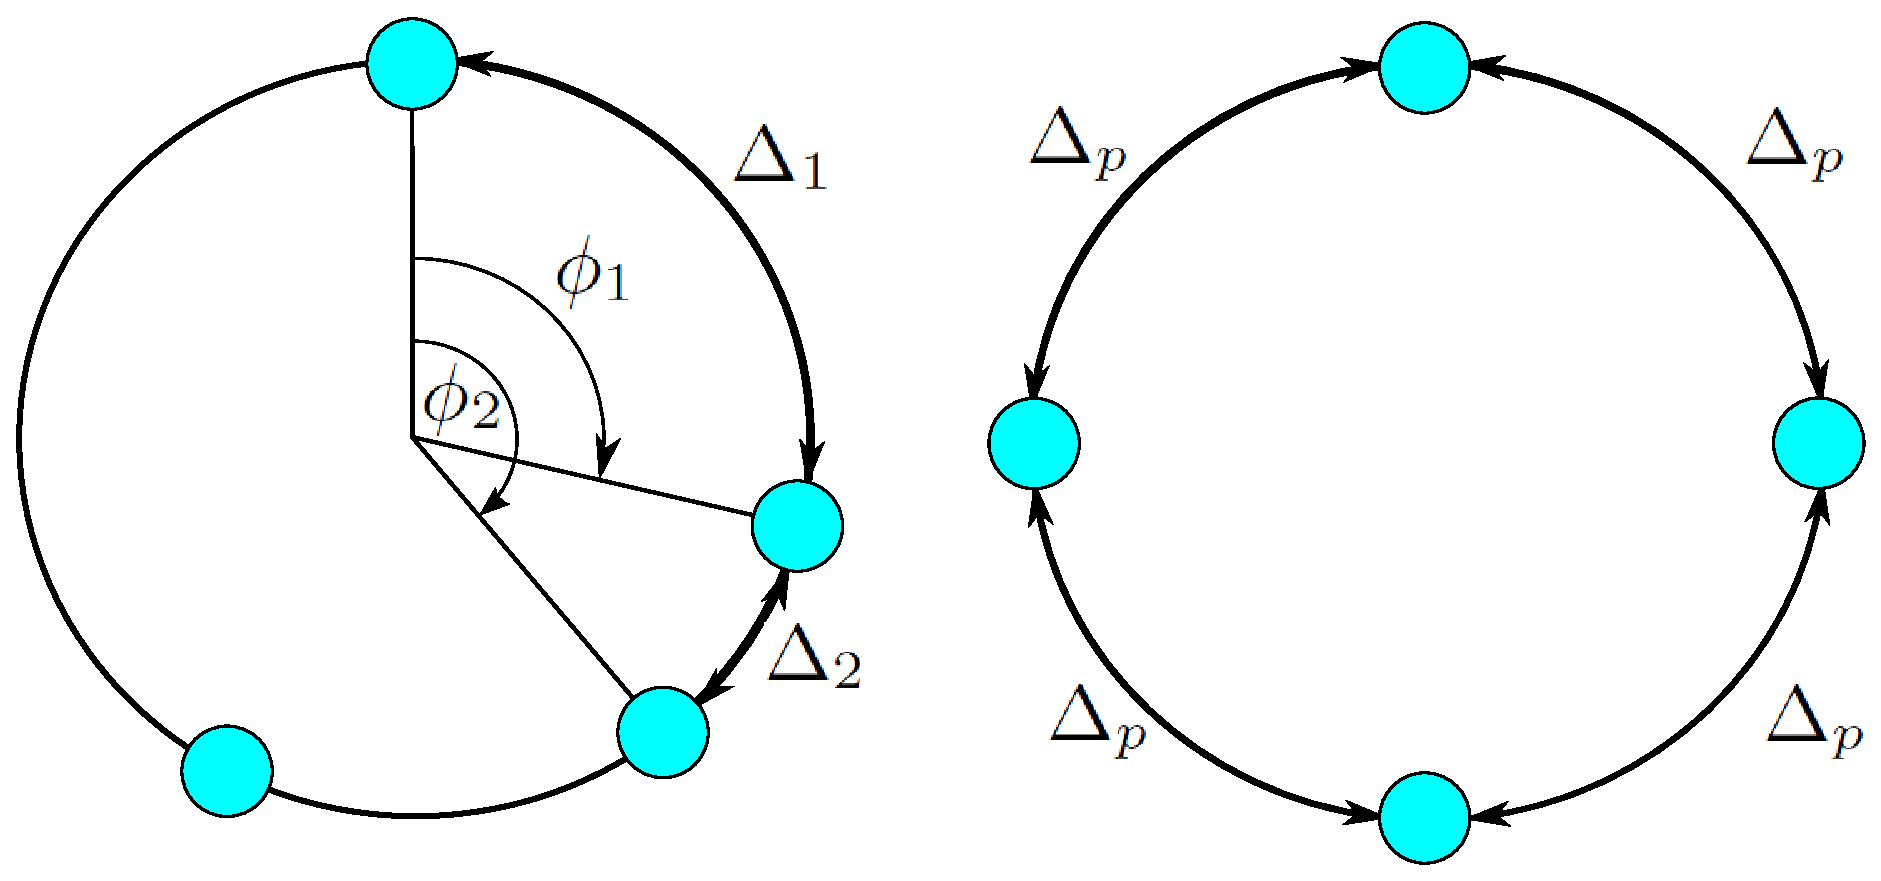
\includegraphics[width=4.0in]{figure/time_circle}
\caption{Desynchronization framework}
\label{fig:time_circle}
\end{figure}

We define terms used in the desynchronization context as follows:

\begin{defn}[Phase]
A phase $\phi_i$ of node $i$ is the time position on the circle of a time period $T$, where $0 \leq \phi_i <  T$ and $T \in \mathbb{R}^+$.
\end{defn}

\begin{defn}[Phase Neighbor]
Node $j$ is a phase neighbor of node $i$ if node $i$ perceives the existence of node $j$ at the phase $\phi_i + \phi_{i,j}$, where $\phi_{i,j}$ is the phase difference between node $j$ and node $i$,
\begin{equation}
\phi_{i,j} = \left\{ 
\begin{array}{l l}
  \phi_j - \phi_i & \quad \mbox{if $\phi_j \geq \phi_i$,}\\
  T - (\phi_i - \phi_j) & \quad \mbox{if $\phi_j < \phi_i$.}\\ \end{array} \right. 
\end{equation}
\end{defn}

\begin{defn}[Next Phase Neighbor]
Node $j$ is the next phase neighbor of node $i$ if $\phi_{i,j} = \min_{k \in S}\{\phi_{i,k}\}$, where $S$ is a set of node $i$'s neighbors. 
%Node $j$ is the next phase neighbor of node $i$ if it has the minimum phase difference among node $i$'s phase neighbors . 
\end{defn}
\begin{defn}[Previous Phase Neighbor]
Node $j$ is the previous phase neighbor of node $i$ if $\phi_{i,j} = \max_{k \in S}\{\phi_{i,k}\}$, where $S$ is a set of node $i$'s neighbors.
%A node $j$ is the next phase neighbor of a node $i$ if it has the maximum phase difference among node $i$'s phase neighbors . 
\end{defn}
\begin{defn}[Desynchrony State]
The system is in the desynchrony state if $\phi_i \neq \phi_j$ for all $i, j \in V$ and  $i \neq j$, where $V$ is a set of nodes in a network that cannot share the same phase.
\end{defn}
\begin{defn}[Perfect Desynchrony State]
The system is in the perfect desynchrony state if it is in the desynchrony state and $\phi_{i,j} = T/N$ for all $i \in V$, $j$ is $i$'s previous phase neighbor, and $N$ is the number of nodes in a network that cannot share the same phase.
\end{defn}

We note that two nodes can share the same phase if they are not within the two-hop communication range of each other.

\section{Related Work}
\label{sec:related}
In this section, we review works in literature. We divide related works into two categories.
The first category is the works on desynchronization in a temporal domain.
The works in this category directly attempt to solve the desynchronization problem in wireless networks.
We compare our work directly to these previous works.
The second category is the works on robotic circular formation. The works in this category do not explicitly attempt to solve the desynchronization problem in wireless networks. However, their works can be abstracted as desynchronization on a spatial domain. These works are the motivation of our desynchronization algorithm.

\subsection{Desynchronization on a Temporal Domain in Wireless Networks}
\label{sec:timedesync}
To the best of our knowledge, DESYNC (\cite{4379660})  is the first to introduce the desynchronization problem. In DESYNC, a node simply attempts to stay in the middle between its previous and next phase neighbors. By repeating this simple algorithm, all nodes will eventually be spread out. However, the error from one phase neighbor is also propagated to the other phase neighbors and indefinitely circulated inside the network. Therefore, DESYNC's error is quite high even after convergence. In contrast, our work relies on all received neighbors information that is robust to the error from one phase neighbor. 
 In  \cite{4663417}, they describe how DESYNC works on multi-hop networks and describe a future extension for DESYNC by exchanging 2-hop neighbors information. 

Designed to converge faster than DESYNC, INVERSE-MS (\cite{4274893}) is an inverse algorithm of the synchronicity work by \cite{MS1990}. 
At a steady state, INVERSE-MS maintains a dynamic equilibrium (\textit{i.e.}, nodes keep changing time positions while maintaining desynchronization). 
However, in INVERSE-MS, the time period is distorted whereas our algorithm does not distort the time period.

In EXTENDED-DESYNC (\cite{MK09DESYNC}), they propose a desynchronization algorithm that is similar to the extension proposed in \cite{4663417}.
Each node sends its one-hop neighbors' relative time information to all of its one-hop neighbors.
Then, the one-hop neighbors relay such information to two-hop neighbors.
Therefore, each node knows 2-hop relative time information.
Consequently, each node can presume that there are two-hop neighbors appearing on the time circle.
Then, each node uses time information of both one-hop and two-hop neighbors and processes with the same algorithm as in DESYNC. Our multi-hop algorithm is partly based on the same idea.

M-DESYNC (\cite{5062256}) is a localized multi-hop desynchronization algorithm that works on a granularity of time slots. The protocol estimates the required number of time slots with a two-hop maximum degree. This estimation helps M-DESYNC converge very fast. However, M-DESYNC requires that all nodes have a global notion of time in order to share the common perception of time slots. Furthermore, M-DESYNC is claimed to work only on acyclic graph networks. On the contrary, our algorithm does not require a global notion of time and can work on both acyclic and cyclic graph networks.

\cite{5062165} propose a simple, lightweight desynchronization algorithm that is also based on a graph coloring model. Unlike M-DESYNC, the algorithm works on general graph networks and does not need the global time. To ensure that the selected time slot does not overlap with others', a node needs to listen to the media for a full time period before claiming the slot. The listening mechanism can only avoid collision with one-hop neighbors but cannot avoid collision with two-hops neighbors (\textit{i.e.}, the hidden terminal problem).
Furthermore, without a common notion of time, the starting time of each slot is quite random. As a result, several time gaps are too small to be used as time slots. This external fragmentation problem reduces resource utilization of the system. Finally, to converge faster, their algorithm overestimates the number of required time slots. Hence, several big time gaps are also left unused and the resource utilization is undoubtedly low. In our work, nodes gradually adapt their phases to be separated from each other as far as possible. Therefore, the external fragmentation problem is reduced. In addition, our algorithm works well on multi-hop networks; each node can avoid collision with two-hops neighbors.

In DESYNC-ORT (\cite{desyncort}), they propose an Orthodontics-inspired desynchronization
algorithm.
In their work, they use information from all one-hop neighbors and attempt to find nodes that are already in corrected time positions and tie them up together.
This method is similar to the Orthodontics method that attempts to tie teeth which are already in corrected positions together.
Their result is better than DESYNC in the term of desynchronization error. 
However, to calculate the correct positions, each node requires to know the total number of nodes in the system in advance. Additionally, the algorithm does not propose to solve the problem in multi-hop networks because nodes in two-hop neighbors can not be tied together with one-hop neighbors. In contrast, our algorithm does not require the total number of nodes in advance. Our algorithm can gradually adapt based on the current number of two-hop neighbors. Additionaly, our algorithm works on multi-hop networks. 

Recently, V-DESYNC (\cite{v-desync}) has been proposed to desynchronize nodes in vehicular ad-hoc networks. Their work has a different objective. They do not focus on fairness (\textit{i.e.}, nodes are not necessary to be equitably separated) because vehicular networks are highly dynamic. In our work, we focus in static wireless sensor networks and attempt to leverage fairness among sensor nodes in resource utilization.

Table \ref{tab:compare} summarizes the advantages and disadvantages of works in this category. The overhead of the proposed algorithm depends on whether the algorithm works on single-hop or multi-hop mode.

\begin{table}
\centering
\begin{tabular}{|c|c|c|c|c|c|c|c|c|} 
\hline
 & \multicolumn{8} {|c|}{Properties} \\  \cline{2-9}
Approach & Period & Time & Equita- & Multi- &  Conver- & Error & Scala- & Over- \\ 
 &  & Synced & ble &  hop	 & gence &  & ble & head \\ 
  &  &  & Spaced  &   &  &  &  &  \\ 
\hline \hline 
DESYNC & Fixed & No & Yes & No & Moderate & High & Poor & Zero  \\ 
  &  &  &  &   &  &  &  &  \\ 
\hline 
INVERSE-MS & Distorted & No & Yes  & No & Fast & Low & Good & Zero \\ 
  &  &  &  &   &  &  &  &  \\ 
\hline 
EXTENDED- & Fixed & No & Yes &  Yes & Moderate & High &  Poor & High \\ 
DESYNC &  &  &  &   &  &  &  &  \\ 
\hline 
M-DESYNC & Fixed & Required & No & Yes & Fast & High & Good & Low \\ 
  &  &  &  &   &  &  &  & \\ 
\hline 
LIGHT-  & Fixed & No & No & Yes & Fast & High & Good & Zero \\ 
WEIGHT &  &  &  &   &  &  &  & \\ 
\hline 
DESYNC-  & Fixed & No & Yes & No & Moderate & Low & Good & Zero \\ 
ORT &  &  &  &   &  &  &  & \\ 
\hline 
V-DESYNC  & Fixed & No & No & No & No & High & Good & Zero \\ 
  &  &  &  &   &  &  &  &  \\ 
\hline 
Proposed & Fixed & No & Yes & Yes & Moderate & Low &  Good & Zero/ \\ 
  &  &  &  &   &  &  &  & Low \\ 
\hline 
\end{tabular} 
\caption{Desynchronization Protocols Comparison}
\label{tab:compare}
\end{table}

\subsection{Desynchronization on a Spatial Domain in Robotics}
\label{sec:spacedesync}
In robotic pattern formation, multiple robots distributedly group and align themselves in geometric patterns such as circle, rectangle, and triangle. Without an explicit argument, robotic pattern formation can be abstracted as desynchronization on a spatial domain. Robots attempt to separate away from each other as far as possible to form such patterns. In other words, robots desynchronize themselves spatially to avoid the collision with each other in the spatial domain.

Several works have done in several pattern formations (\cite{suzuki-96}, \cite{suzuki-99}). However, the pattern formation that is similar to desynchronization on the temporal domain is the formation on a closed ring. 
Figure \ref{fig:robotic-closed-ring} illustrates the robotic formation on a closed ring. In Figure \ref{fig:closedring}, initially, robots are randomly placed on any position on the closed ring. The perfect configuration of the formation is illustrated in Figure \ref{fig:closedring-perfect}. Robots are equivalently separated away on the ring. 

\begin{figure*}[!t]
\centerline {
	\subfloat[]{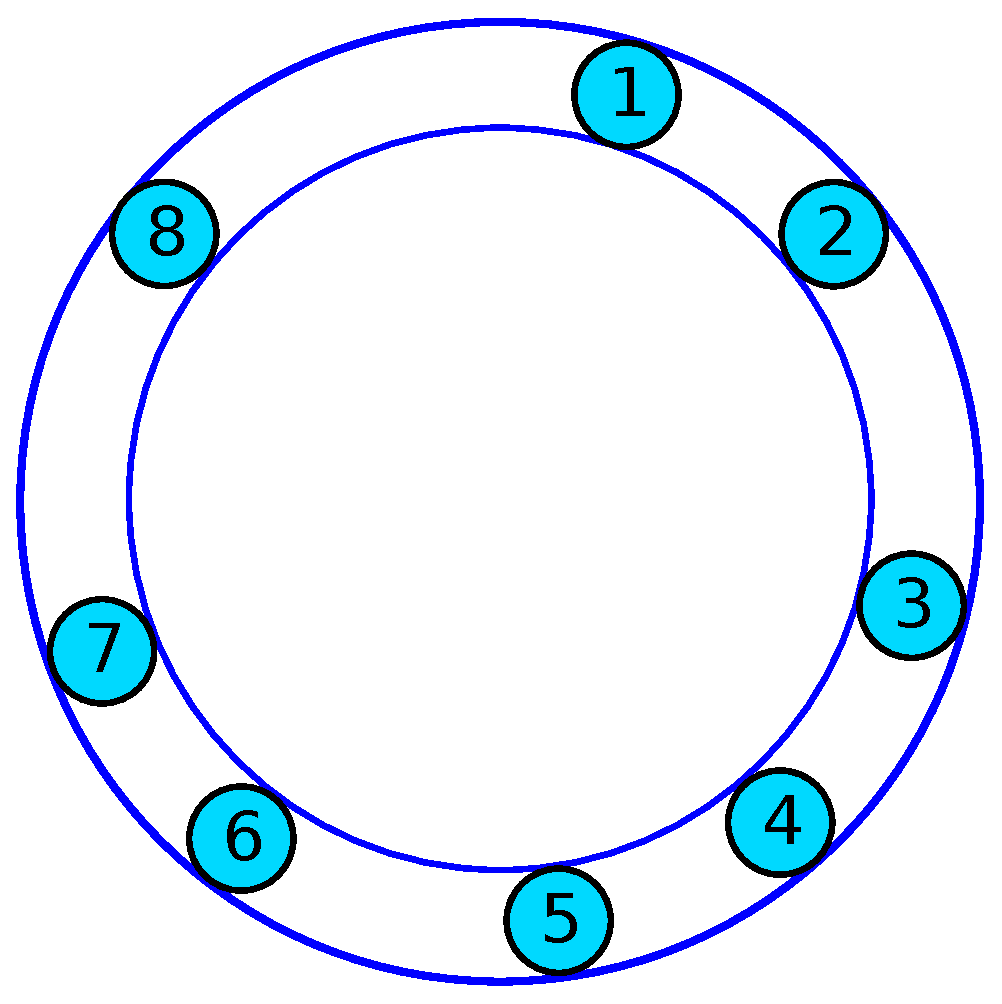
\includegraphics[width=2in]{figure/robotic-closed-ring}%
	\label{fig:closedring}}
	\hfil
	\subfloat[]{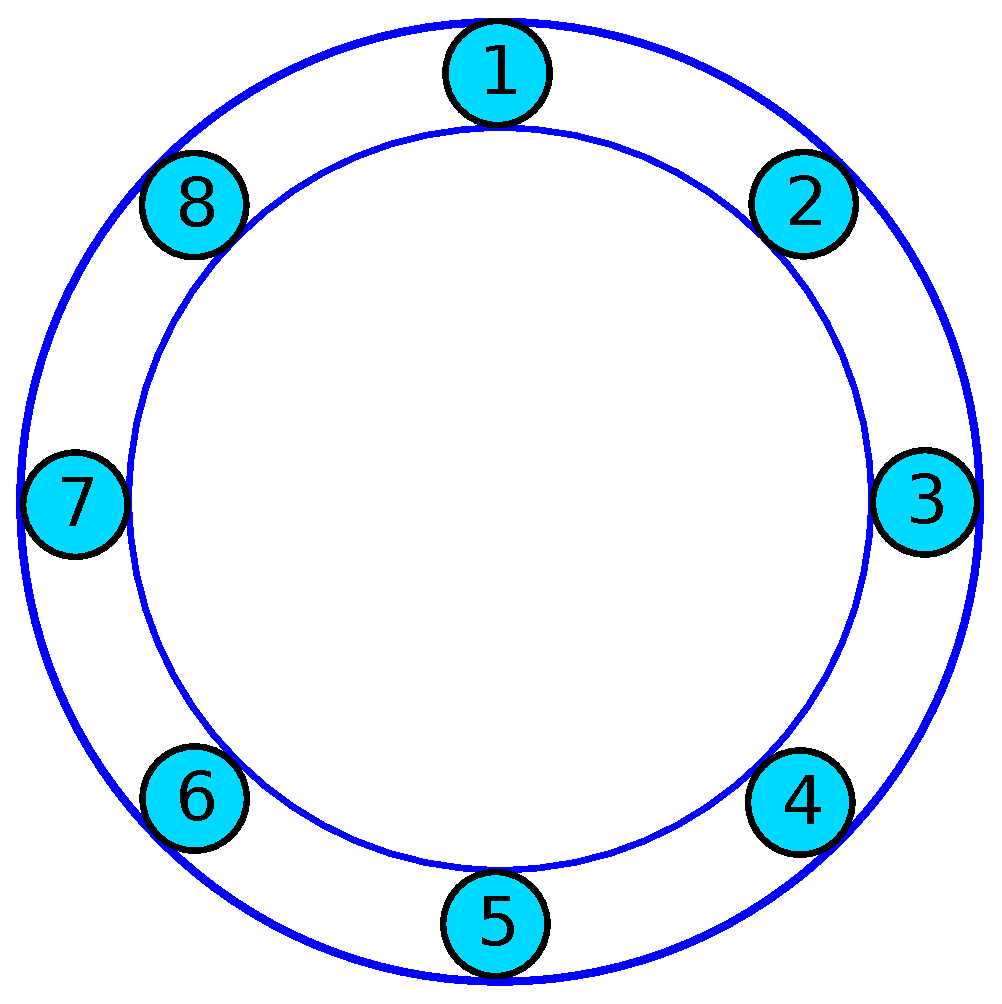
\includegraphics[width=2in]{figure/robotic-closed-ring-perfect}%
	\label{fig:closedring-perfect}}
}
\caption{Robotic pattern formation on a closed ring. (a) Robots are randomly placed on a closed ring. (b) In the perfect configuration, robots are equitably separated from each other. }
\label{fig:robotic-closed-ring}
\lofcont
\end{figure*}

Several previous works such as \cite{defago04}, \cite{cohen-08}, and \cite{flocchini-08} have proposed algorithms that are similar to each other for robotic formation on a closed ring. These works assume robots have limited visibility range. Each robot attempts to adjust its position to the middle between two nearest robots on its left side and right side (Figure \ref{fig:closedring-desync}). In these works, they prove that this simple algorithm eventually converges to the perfect configuration (Figure \ref{fig:closedring-desync-perfect}).

\begin{figure*}[!t]
\centerline {
	\subfloat[]{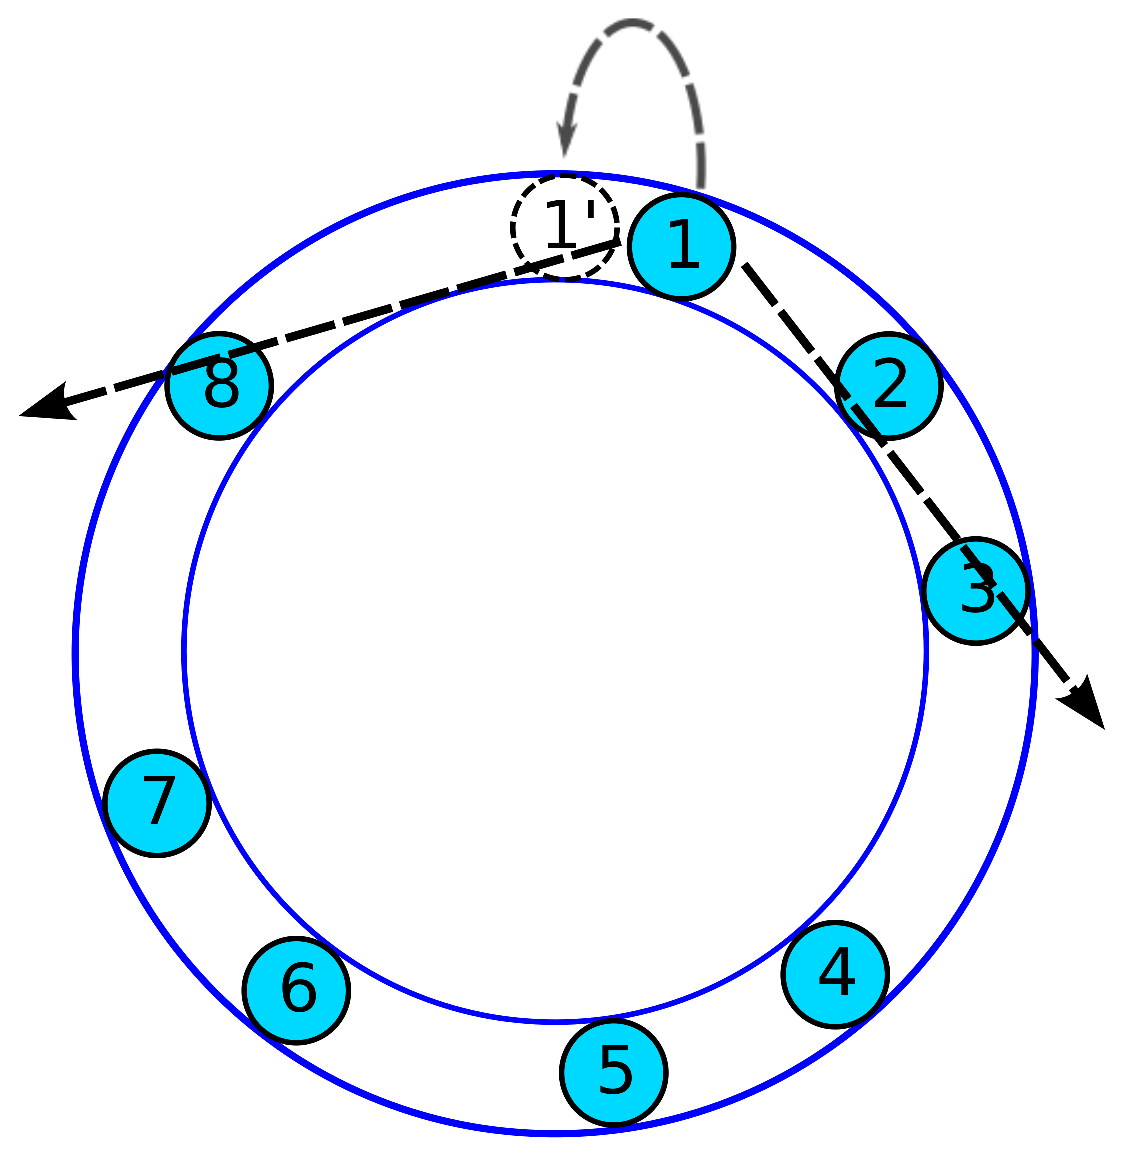
\includegraphics[width=2in]{figure/robotic-closed-ring-desync}%
	\label{fig:closedring-desync}}	
	\hfil
	\subfloat[]{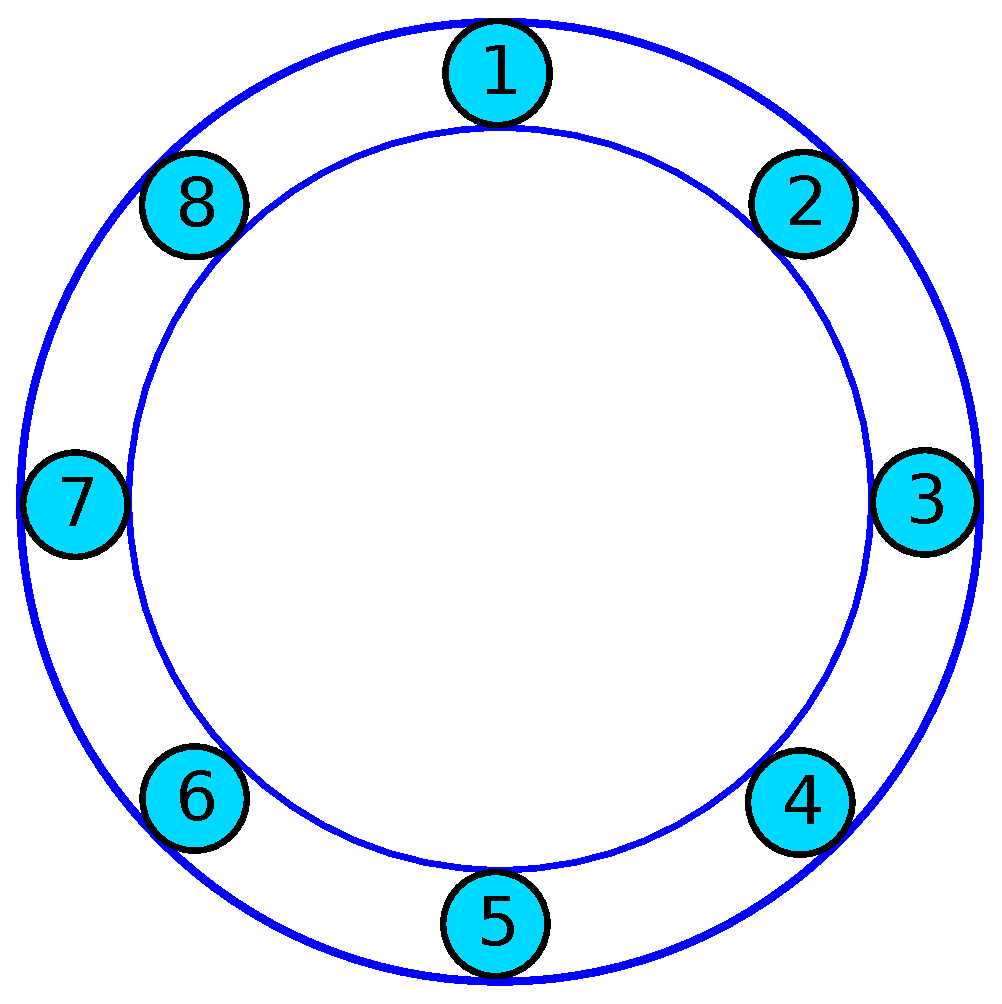
\includegraphics[width=2in]{figure/robotic-closed-ring-desync-perfect}%
	\label{fig:closedring-desync-perfect}}	
}
\caption{Moving to the midpoint algorithm. (a) Each robot moves to the midpoint between two nearest visible neighbors. (b) The algorithm converges to the perfect configuration.}
\label{fig:robotic-closed-ring-desync}
\lofcont
\end{figure*}

In \cite{4141997}, heterogeneous robots are distributedly grouped into teams that are equally spread out to cover the monitored area. Each robot has no global knowledge of others’ absolute positions but can detect relative positions of the others with respect to itself as well as the type of the others. 
To form a circle, an artificial force is used as an abstraction for velocity adaptation of a robot. 
Robots of different types have attracting forces to each other. Conversely, robots of the same type have repelling forces. As a result, the circle of heterogeneous robots will be formed and robots are nicely spaced on the circle  (see Figure \ref{fig:circular_formation}). This work inspires our desynchronization algorithm.

\begin{figure}[!t]
\centering
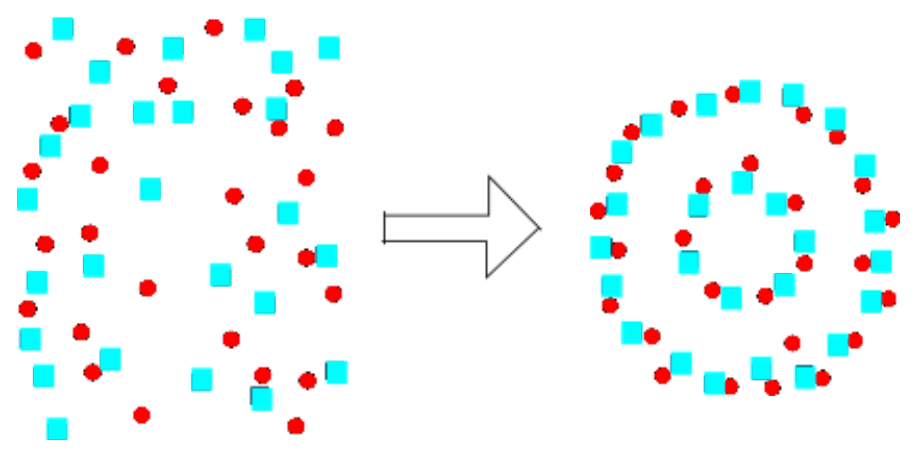
\includegraphics[width=5.0in]{figure/robo_new}
\caption{Results of Robotic Circular Formation. Robots with two different types form the circle.}
\label{fig:circular_formation}
\end{figure}

\subsection{Others}
\label{sec:tdma}
Other works that are related to desynchronization protocols are distributed Time Division Multiple Access (TDMA) protocols. Distributed TDMA protocols are similar to M-DESYNC (\cite{5062256}); their protocols work on a granularity of time slots. 
As same as M-DESYNC, most of distributed TDMA protocols such as TRAMA (\cite{trama}), Parthasarathy \cite{Parthasarathy}, ED-TDMA (\cite{edtdma}), and Herman (\cite{herman}) assume time is already slotted or all nodes are synchronized to achieve the same global clock. 
%Some distributed TDMA protocols do not require time synchronization. However, they require more states and incur control message overhead. For example, DRAND \cite{4803842}  requires the control overhead for sending request, reject, release, and grant messages. 
In our work, we do not require time synchronization and do not assume already slotted time.

\section{Motivation}
\label{sec:motivation}
We observe that the desynchronization framework on the temporal domain is similar to the robotic circular formation which can be abstracted as the desynchronization on the spatial domain.
In the desynchronization framework on the temporal domain, a node (like a robot) does not have a global notion of time but each node can measure relative time differences with other nodes.
The circle of robots is similar to our circle of the time period. 
The distribution of robots can be mapped to the distribution of nodes on the time circle. 
The robotic circular formation of \cite{4141997} inspires us to design a novel desynchronization algorithm for wireless sensor networks based on an \textit{artificial force field}.
If we abstract the nodes on a time circle as the robots of the same type, the nodes will repel each other and keep time intervals from their neighbors as far as possible.
Once all received forces are balanced, nodes are equally spread out on the time circle.

The desynchronization algorithm based on the artificial force field can be classified as a \textit{Physicomimetics} algorithm.
A physicomimetics algorithm is an algorithm that imitates principles of physics and can be called \textit{Artificial Physics} or \textit{Virtual Physics} (\cite{physicomimetics}). To the best of our knowledge, physicomimetics was introduced in \cite{810278} for distributed control of large collections of agents. Then, physicomimetics has been applied mostly in the field of robotics for geometric pattern formation and optimizations such as in \cite{swarm}, \cite{artphysics}, and \cite{4141997}.
Due to the framework of desynchronization is similar to the framework of robotic geometric pattern formation, we believe that the physicomimetics approach can also solve the desynchronization problem in the temporal domain as well. 
Therefore, this dissertation presents how physics principles can be imitated to solve the desynchronization problem for wireless sensor networks.

\chapter{Physicomimetics Desynchronization Algorithm for Single-hop Networks}
\label{chap:algo}

\section{Introduction}
\label{sec:intro-dwarf}
As we mentioned in the previous chapter, physicomimetics algorithms have been widely used for the robotic pattern formation that can be abstracted as desynchronization in the spatial domain.
One of such algorithms is that of \cite{4141997}. In their work, robots are in an artificial force field. Robots with the same type repel each other to form themselves into a circular shape. 

Inspired by their work, in this chapter, we present a novel physicomimetics desynchronization algorithm called \textit{DWARF} (Desynchronization With an ARtificial Force field) for single-hop wireless sensor networks.
Each neighboring node has artificial forces to repel other nodes to perform tasks at different time phases. Nodes with closer time phases have stronger forces to repel each other in the time domain. Each node adjusts its time phase proportionally to its received forces. Once the received forces are balanced, nodes are desynchronized

DWARF has the following key contributions:
\begin{itemize}
\item DWARF is a distributed desynchronization algorithm using time phases of all neighbors to achieve the desyncrhony state. 
\item DWARF uses only local information but achieves a global state.
\item DWARF does not require time synchronization, does not assume already slotted time, and does not incur any control message overhead.
\item DWARF is simple due to low complexity in terms of computation and memory. Therefore, it is suitable for resource-constraint networks, such as wireless sensor networks. Additionally, message complexity is low because the algorithm relies on the timing of the message, not information inside the message.
\item We have implemented and evaluated DWARF on TOSSIM, a simulator for wireless sensor networks. Our results indicate that DWARF scales well with network size and outperforms DESYNC significantly by achieving 10 - 63\% reduction in desynchronization error.
\end{itemize}
Therefore, we believe that DWARF can be a primer for various applications and can be extended for multi-hop networks which will be later described in Chapter \ref{chap:multihop}.

In the next section, we present the concept of an artificial force field which is the crucial concept of our desynchronization algorithm.

\section{Artificial Force Field}
\label{sec:forcefield}
An artificial force field is an analogy to the circle of a time period.
Nodes are in the same force field if they can communicate with each other. 

If node $i$ and node $j$ are on the same force field, they have repelling forces to push one another away. 
A closer pair of nodes has a higher magnitude of force than a farther pair does.
The time interval between two nodes is derived from the phase difference between them.
If two nodes have a small phase difference, they have a high magnitude of force and vice versa.
In other words, a repelling force is an inverse of a phase difference between two nodes:
\begin{equation}
f_{i,j} = - \frac{1}{\Delta \phi_{i,j} / T} , \Delta \phi_{i,j} \in (-\frac{T}{2}, \frac{T}{2}),
\label{eq:force}
\end{equation}
where $f_{i,j}$ is the repelling force from node $j$ to node $i$ on a time period $T$ and $\Delta \phi_{i,j}$ is the phase difference between node $i$ and $j$.
We note that $\Delta \phi_{i,j}$ is not equal to 0 because if two nodes fire at the same time, their firings collide and two nodes do not record other's firing. Additionally, at $T/2$ or $-T/2$, a node does not repel an opposite node because they are balanced.

A repelling force can be positive (clockwise repelling) or negative (counterclockwise repelling).
A positive force is created by a node on the left half of the circle relative to the considered node whereas a negative force is created by a node on the right half.
Figure \ref{fig:force_field} represents a field of repelling forces on node 1. 

\begin{figure}[!t]
\centering
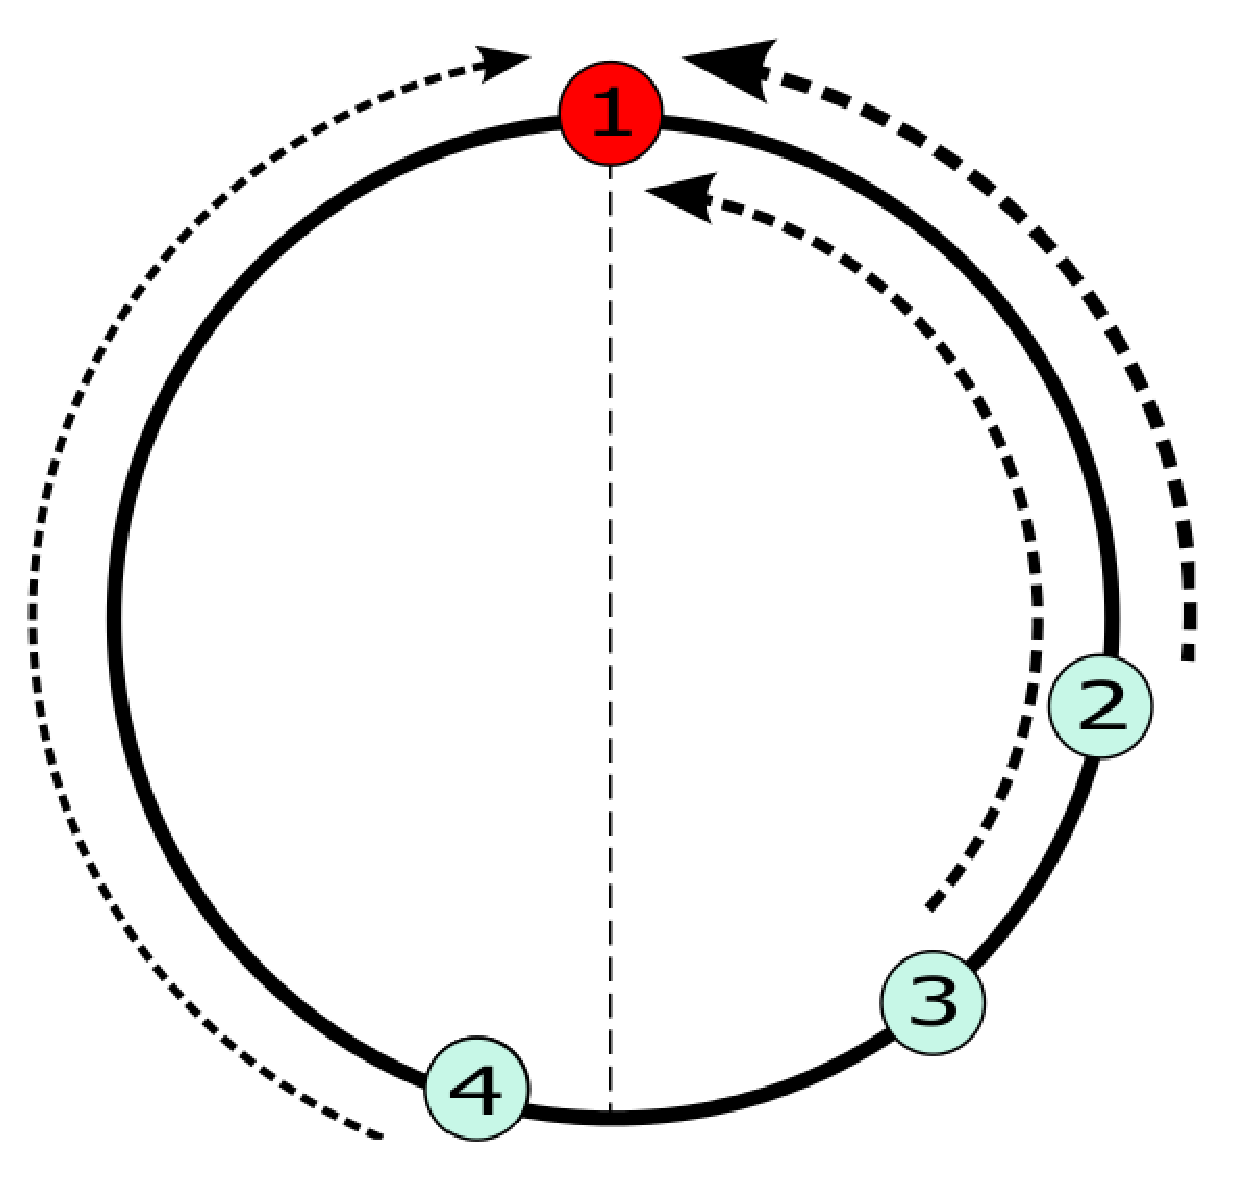
\includegraphics[width=2.2in]{figure/forcefield}
\caption{Artificial Force Field. Arrow lines represent repelling forces from node 2, 3, and 4 to node 1. A shorter and thicker line is a stronger force. A force from node 4 is a positive force and two forces from node 2 and 3 are negative forces.}
\label{fig:force_field}
\end{figure}

Each node in the force field moves to a new time position or phase proportional to the total received force.
Given $n$ nodes in a force field, the total force on a node $i$ is the following:
\begin{equation}
\mathcal{F}_i = \sum_{\substack{j=1\\ j \neq i}}^{n}{f_{i,j}}.
\label{eq:fsum}
\end{equation}
Eventually, nodes reach an equilibrium state whereby the total force of the system is close to zero and each pair of phase neighboring nodes has the same time interval.
This equilibrium state also indicates the perfect desynchrony state because all nodes are equally spaced on the time circle.

\section{Algorithm}
\label{sec:algo}
We assume that, initially, nodes are not desynchronized. 
Each node sets a timer to fire in $T$ time unit.
After setting the timer, each node listens to all neighbors until its timer expires.

When receiving a firing message from its neighbor, the (positive or negative) repelling force from that neighbor is calculated based on the phase difference.
When the timer expires, a node broadcasts a firing message to neighbors. 
Then, the node calculates a new time phase to move on the circle based on the summation of forces from all neighbors and sets a new timer according to the new time phase.

Reasonably, one may wonder how far a node should move or adjust its phase.
In our work, given the total received force $\mathcal{F}_i$, the node $i$ adjusts to a new time phase $\phi_i^{'}$,
\begin{equation}
\phi_i^{'} = (\phi_i + K\mathcal{F}_i) \mod T,
\label{eq:newphase}
\end{equation} 
where $\phi_i$ is the current phase of the node $i$.

Undoubtedly, the proper value of the coefficient $K$ leads to the proper new phase.
The value of $K$ is similar to a step size which is used in artificial intelligence techniques. 
Therefore, if the value of $K$ is too small, the system takes much time to converge. 
On the other hand, if the value of $K$ is too large, the system may overshoot the optimal value and does not converge. 
We observe that, given the same time period, fewer nodes in the system result in bigger phase difference between two phase neighbors. To be desynchronized, nodes in sparse networks must make a bigger adjustment to their time phases than nodes in dense networks must.
Therefore, the same total received force should have a bigger impact on a node in sparse networks than on a node in dense networks. 
To reflect this observation, the coefficient $K$ is inversely proportional to a power of the number of nodes $n$,
\begin{equation}
K = c_1 \times n^{-c_2}, \text{ where } c_1, c_2 \geq 0.
\end{equation}

Therefore, we have conducted an experiment to find the proper value of $c_1$ and $c_2$. 

We set a time period $T$ to 1000 and vary the number of nodes.
In the specific number of nodes, we first simulate to see the trend of the value $K$ that leads to small errors. 
Then, we select a range of good $K$ values. 
After that, we simulate 100 times to obtain the average desynchronization error for each $K$ value. 
In each simulation, we randomly set an initial phase of each node between 0 and $T$ (period value). 
Finally, we select the $K$ value that results in the lowest error. 
After getting the proper $K$ value for each number of nodes, we plot the relation between $K$ and the number of nodes (Figure \ref{fig:relation_k_n}) and use a mathematical tool to calculate the power regression. The obtained relation function between $K$ and $n$ (the trendline in Figure \ref{fig:relation_k_n}) consists of $c_1$ and $c_2$  values as follows:
\begin{equation}
K = 38.597 \times n^{-1.874}.  \nonumber
\end{equation}
However, this $K$ value is derived by setting $T$ equal to 1000. 
Therefore, for arbitrary $T$, 
\begin{equation}
K = 38.597 \times n^{-1.874} \times \frac{T}{1000}.
\end{equation}
\begin{proof}
From Equation \ref{eq:fsum} and \ref{eq:newphase}, the phase of node $j$ is adjusted by $K\mathcal{F}_{j} = K\sum_{i \neq j}^n f_{i,j} = \sum_{i \neq j}^n K f_{i,j}$.
Therefore, we can analyze the value of $K$ from only single force $f_{i,j}$.

\begin{figure}[!t]
\centering
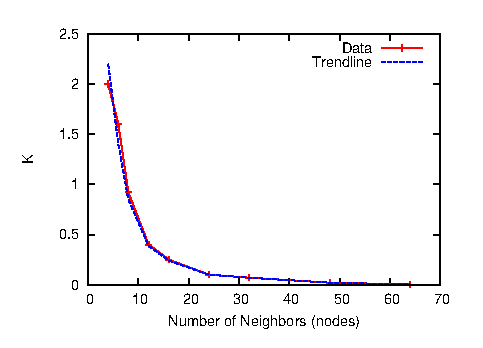
\includegraphics[width=3.5in]{figure/k-trendline}
\caption{Relation of the coefficient $K$ with a number of nodes $n$}
\label{fig:relation_k_n}
\end{figure}

For a time circle of a period $T_{p}$, let $\theta_{p}$ be an angle between two nodes on the circle and $\Theta_{p}$ be an angle between the new adjusted phase and the old phase based on a single force where $\theta_{p}, \Theta_{p} \in (0, 2\pi)$. %and let its value equal to a normalized phase difference $\Delta \phi_{i,j} / T_{p}$ and $\theta^{'}_{p}$ be a new angle after adjustment.
Hence,
\begin{equation}
\frac{\theta_{p}}{2\pi}  = \frac{\Delta \phi_{i,j}}{T_p},
\label{eq:theta}
\end{equation}
and 
\begin{equation}
\frac{\Theta_{p}}{2\pi}  = \frac{Kf_{i,j}}{T_p}.
\label{eq:Theta}
\end{equation}
If $\theta_1$ of $T_1$ equals to $\theta_2$ of $T_2$, both of them should be adjusted with the same angle amount $\Theta_{1}$ = $\Theta_{2}$. 
Thus, from Equation \ref{eq:Theta},
\begin{alignat}{2}
\Theta_1 =&  \text{ } \Theta_2 \nonumber \\
\frac{K_{1} f_{i,j(1)}}{T_1} =& \text{ } \frac{K_{2} f_{i,j(2)}}{T_2}.  \nonumber
\end{alignat}
From Equation \ref{eq:force} and \ref{eq:theta}, $f_{i,j} = \frac{1}{\Delta \phi_{i,j} / T_{p}} = \frac{2\pi}{\theta_{p}}$, consequently,
\begin{alignat}{2}
\frac{K_{1}2\pi}{T_1\theta_1} =& \text{ } \frac{K_{2}2\pi}{T_2\theta_2}  \nonumber \\
\frac{K_{1}}{T_1} =& \text{ } \frac{K_{2}}{T_2}  \nonumber \\
K_2=& \text{ } K_{1} \frac{T_2}{T_1}.  \label{eq:k-k}
\end{alignat}
At $T = 1000$, we get $K = 38.597 \times n^{-1.874}$.
Therefore, from Equation \ref{eq:k-k}, for arbitrary $T$,
\begin{equation}
K = 38.597 \times n^{-1.874} \times \frac{T}{1000}. \nonumber
\end{equation}
\end{proof}


All nodes in the artificial force field (in the period circle) iteratively run the same algorithm until the force is balanced (\textit{i.e.}, all nodes are in the desynchrony state).
The pseudo-code of this algorithm is shown in Figure \ref{fig:pseudocodedwarf}.

\begin{figure}[!t]
\begin{algorithmic}[1]
	\STATE \textbf{Initialization}  
  	\STATE $T = TimePeriod$ \COMMENT{Configurable Time Period}
  	\STATE $n = 1$ \COMMENT{Number of receiving messages including itself}
  	\STATE $\mathcal{F} = 0$ \COMMENT{Force Summation}
  	\STATE $lastFiringTime = localTime$
  	\STATE $currentPhase = localTime$ modulo $T$
  	\STATE Set a firing timer to be $T$ unit time
  	\newline
  	
  	\STATE \textbf{Upon timer firing}
    \STATE Broadcast a firing message to neighbors
    \STATE $lastFiringTime = localTime$
  	\STATE $currentPhase= localTime$ modulo $T$
    \STATE $K = 38.597 \times n^{-1.874} \times \frac{T}{1000}$
    \STATE $newPhase = currentPhase + (K \times \mathcal{F})$
    \IF{$newPhase < 0$}
    	\STATE $newPhase = T + newPhase$
	\ENDIF
    \STATE Set a firing timer to be fired at ($newPhase$ modulo $T$)
   	\STATE $\mathcal{F} = 0$
   	\STATE $n = 1$
 	\newline
 	   
    \STATE \textbf{Upon receiving a firing message}
    \STATE $n = n + 1$
    \STATE $phaseDiff = localTime - lastFiringTime$
    \IF{$phaseDiff == 0.5T$} 
    	\STATE $\mathcal{F} = \mathcal{F} + 0$ \COMMENT{Balanced force}
    \ELSIF{$phaseDiff < 0.5T$} 
    	\STATE $\mathcal{F} = \mathcal{F} + |\frac{1}{phaseDiff / T}|$  \COMMENT{Positive force}
   	\ELSE 
   		\STATE $\mathcal{F} = \mathcal{F} - |\frac{1}{(T - phaseDiff) / T}|$ \COMMENT{Negative force}
    \ENDIF
\end{algorithmic}
\caption{Pseudocode of DWARF algorithm}
\label{fig:pseudocodedwarf}
\end{figure}

\section{Evaluation}
In this section, we evaluate the performance of our proposed algorithm and compare with DESYNC (\cite{4379660}) because DESYNC and our algorithm share the same goal and requirements. Particularly, they do not require time synchronization, do not assume already slotted time, do not need to look into the packet content, and do not incur control packets but still achieve equivalent time spaces. Other protocols (\textit{e.g.}, M-DESYNC (\cite{4274893}), Lightweight desynchronization (\cite{5062165})) assume different requirements. Therefore, we only discuss our differences with such protocols in Chapter \ref{chap:related}.

The performance metrics in this evaluation are desynchronization error and convergence time. The former indicates how close the current state is to the perfect desynchrony state. The latter indicates how fast the algorithm converges.

\subsection{Evaluation Environment}
We implement DWARF on TinyOS 2.1.2 (\cite{levis-tinyos-04}), an operating system for wireless sensor networks
and evaluate the protocol on TOSSIM (\cite{levis-tossim-03}), a TinyOS simulator.
We vary the one-hop network size from 4 to 96 nodes.
Each node periodically fires a message that contains only application data with no extra control overhead.
%The message does not contain any overhead. 
This zero overhead is the advantage of both DWARF and DESYNC because, to avoid collision, a node only needs to know the timing of the firing rather than the control information inside a packet. 
In our simulation, for both DWARF and DESYNC, we use a 2-byte node ID and a 2-byte counter as the data. However, we do use the regular 11-byte CC2420 header for TOSSIM.
Therefore, we do not measure the overhead in our evaluation.
We set the time period to 1,000 milliseconds and compare our result with that of DESYNC.
Initially, the phase of each node is random in a range of 0 to 1,000.

\subsection{Varying Step Size in DESYNC}
\label{sec:varystepsize}
In \cite{4379660}, they choose the step size of DESYNC to be 0.95. In this section, we begin by varying the step size of DESYNC to confirm that the step size 0.95 is a proper and fair value for DESYNC to compare with DWARF in our investigated scenario.
Figure \ref{fig:desync-vary-small}, \ref{fig:desync-vary-medium}, and \ref{fig:desync-vary-large} show the results of varying step size from 0.10 to 0.95.
\begin{figure*}%
\centering
	\subfloat[$\alpha$ = 0.10]{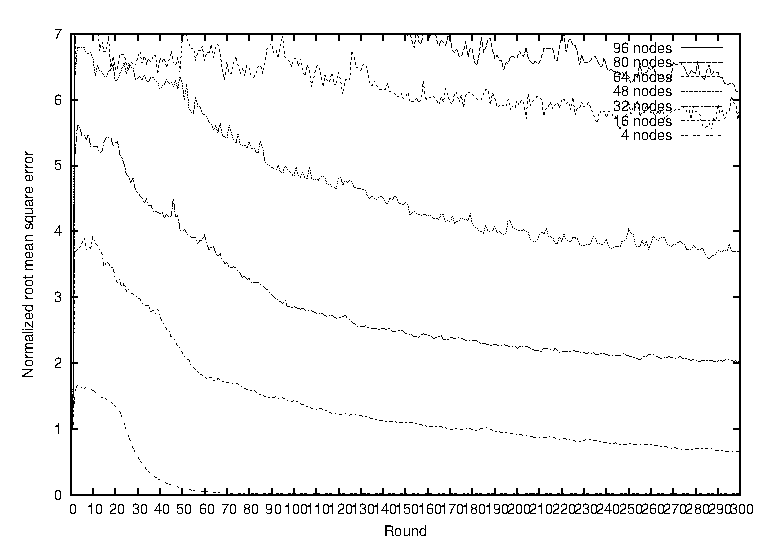
\includegraphics[width=2.5in]{figure/desync-0-10}%
	\label{fig:alpha010}}
	\subfloat[$\alpha$ = 0.15]{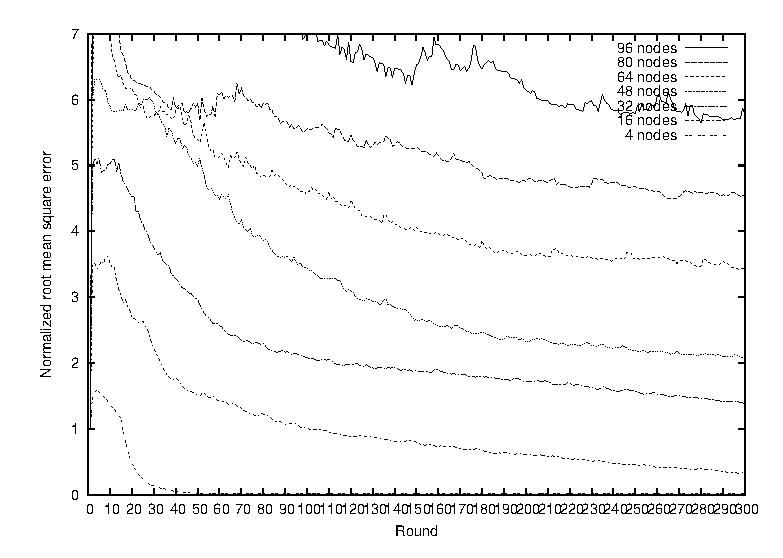
\includegraphics[width=2.5in]{figure/desync-0-15}%
	\label{fig:alpha015}}
    \hspace{8pt}%
	\subfloat[$\alpha$ = 0.20]{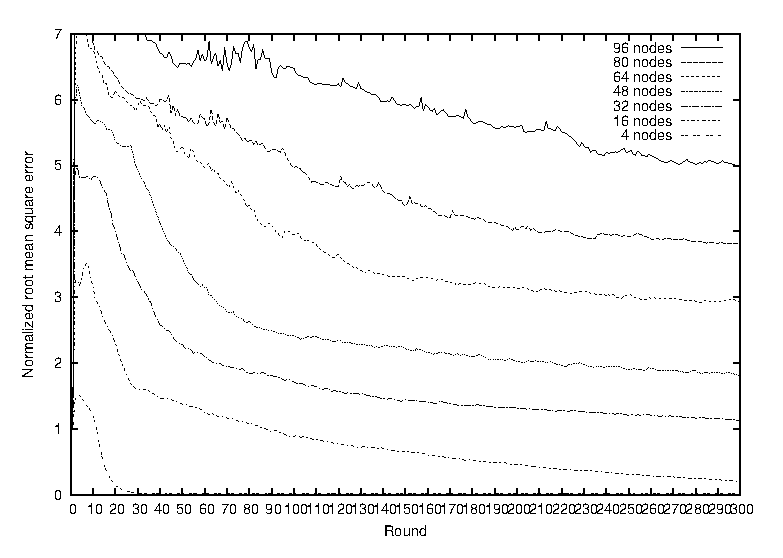
\includegraphics[width=2.5in]{figure/desync-0-20}%
	\label{fig:alpha020}}
	\subfloat[$\alpha$ = 0.25]{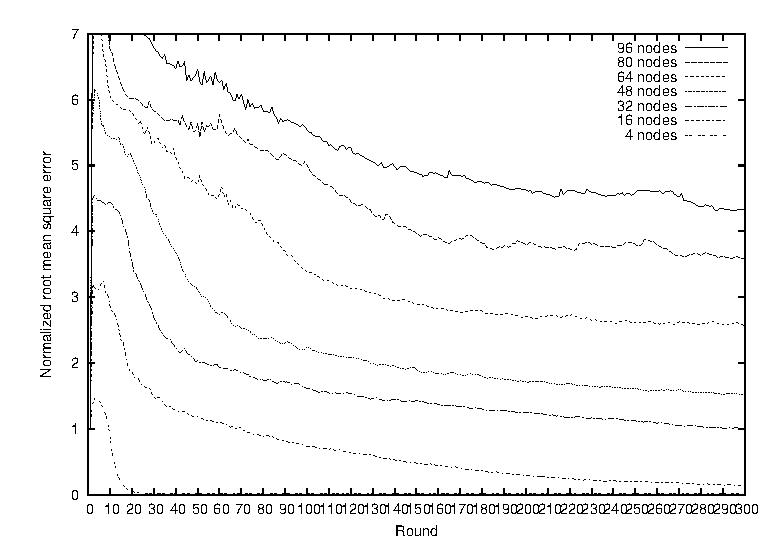
\includegraphics[width=2.5in]{figure/desync-0-25}%
	\label{fig:alpha025}}
    \hspace{8pt}%
	\subfloat[$\alpha$ = 0.30]{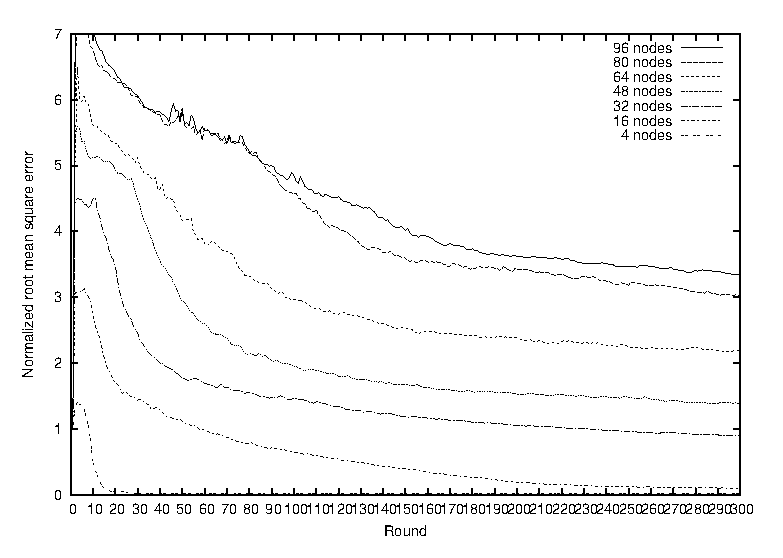
\includegraphics[width=2.5in]{figure/desync-0-30}%
	\label{fig:alpha030}}
	\subfloat[$\alpha$ = 0.35]{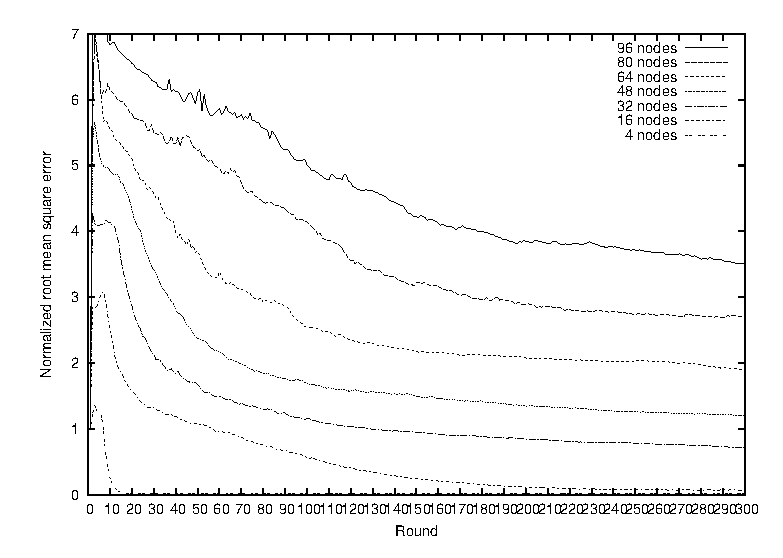
\includegraphics[width=2.5in]{figure/desync-0-35}%
	\label{fig:alpha035}}
\caption{DESYNC: Varying step size from 0.10 to 0.35}%
\label{fig:desync-vary-small}%
\lofcont
\end{figure*}

\begin{figure*}%
\centering
	\subfloat[$\alpha$ = 0.40]{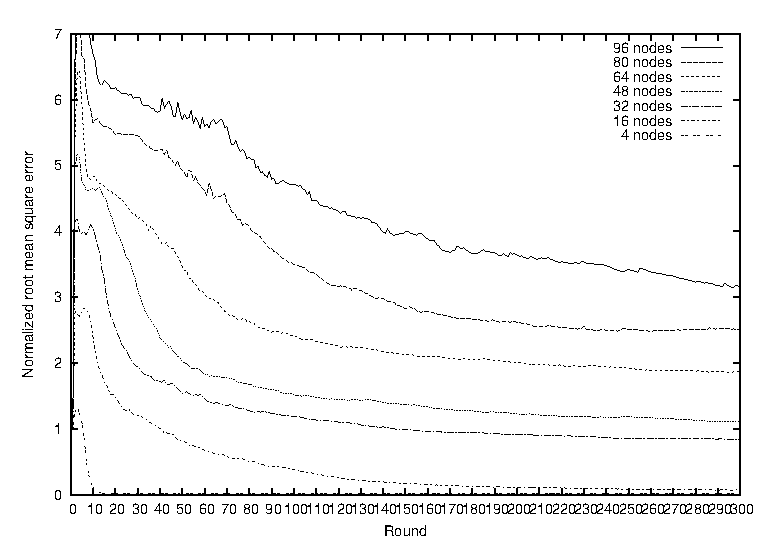
\includegraphics[width=2.5in]{figure/desync-0-40}%
	\label{fig:alpha040}}
	\subfloat[$\alpha$ = 0.45]{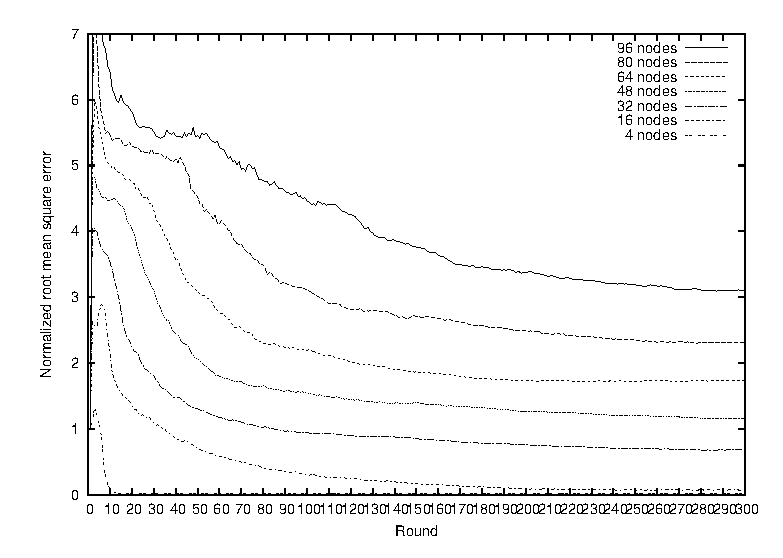
\includegraphics[width=2.5in]{figure/desync-0-45}%
	\label{fig:alpha045}}
    \hspace{8pt}%
	\subfloat[$\alpha$ = 0.50]{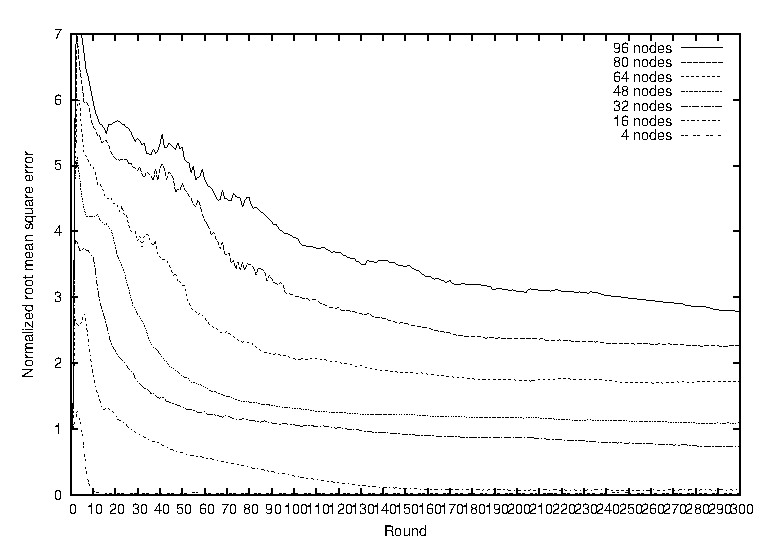
\includegraphics[width=2.5in]{figure/desync-0-50}%
	\label{fig:alpha050}}
	\subfloat[$\alpha$ = 0.55]{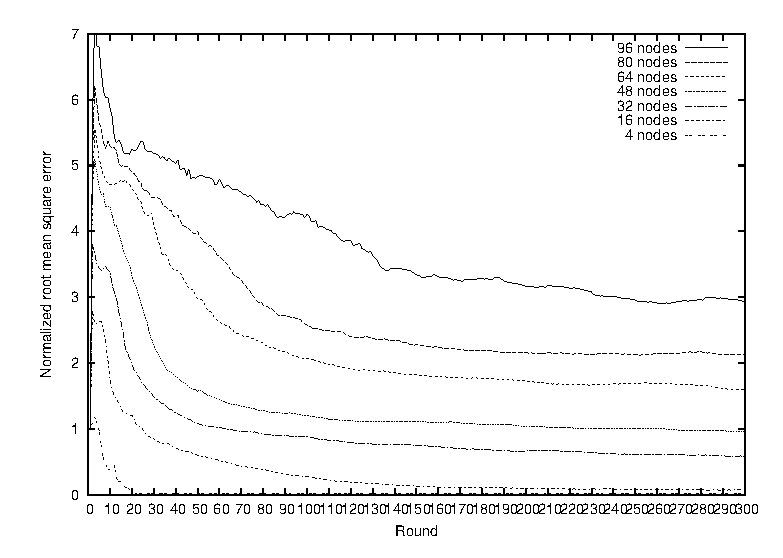
\includegraphics[width=2.5in]{figure/desync-0-55}%
	\label{fig:alpha055}}
    \hspace{8pt}%
	\subfloat[$\alpha$ = 0.60]{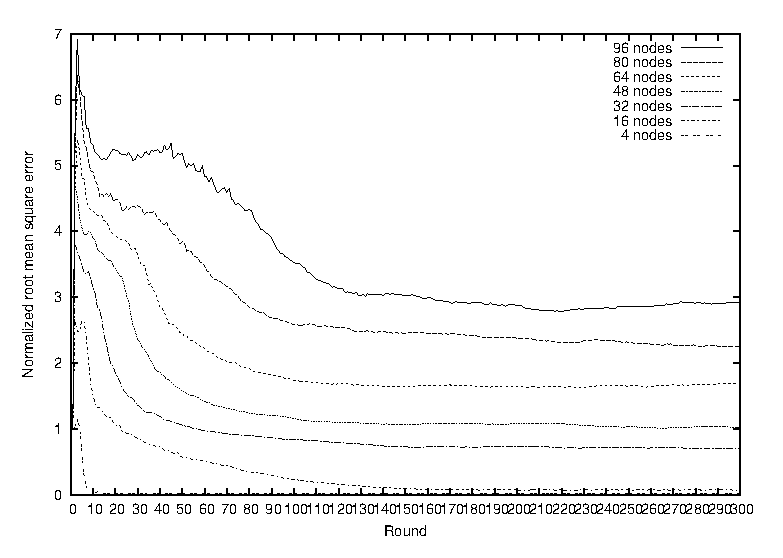
\includegraphics[width=2.5in]{figure/desync-0-60}%
	\label{fig:alpha060}}
	\subfloat[$\alpha$ = 0.65]{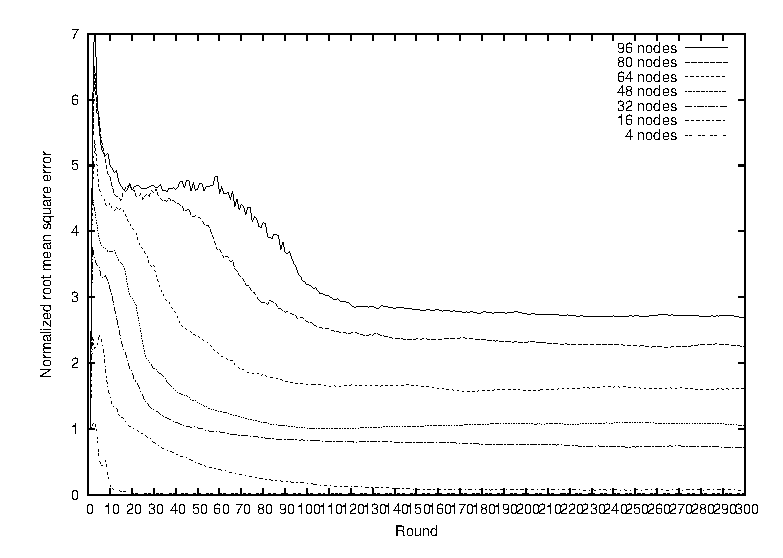
\includegraphics[width=2.5in]{figure/desync-0-65}%
	\label{fig:alpha065}}
\caption{DESYNC: Varying step size from 0.40 to 0.65}%
\label{fig:desync-vary-medium}%
\lofcont
\end{figure*}

\begin{figure*}%
\centering
	\subfloat[$\alpha$ = 0.70]{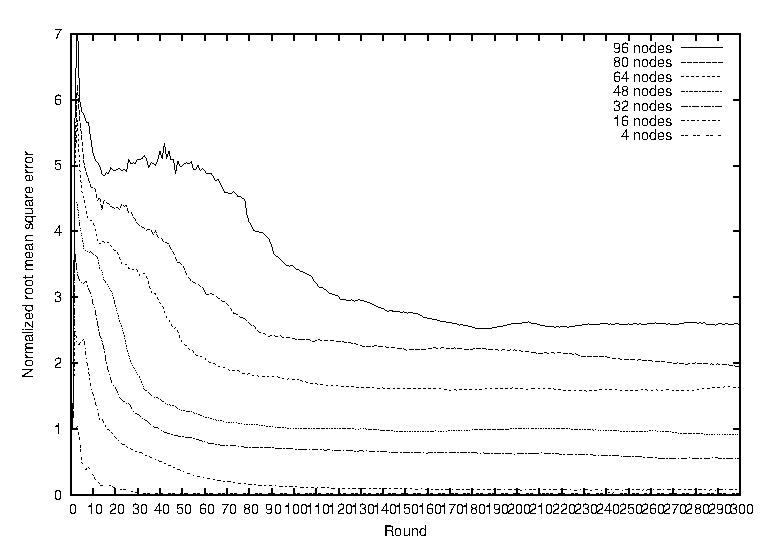
\includegraphics[width=2.5in]{figure/desync-0-70}%
	\label{fig:alpha070}}
	\subfloat[$\alpha$ = 0.75]{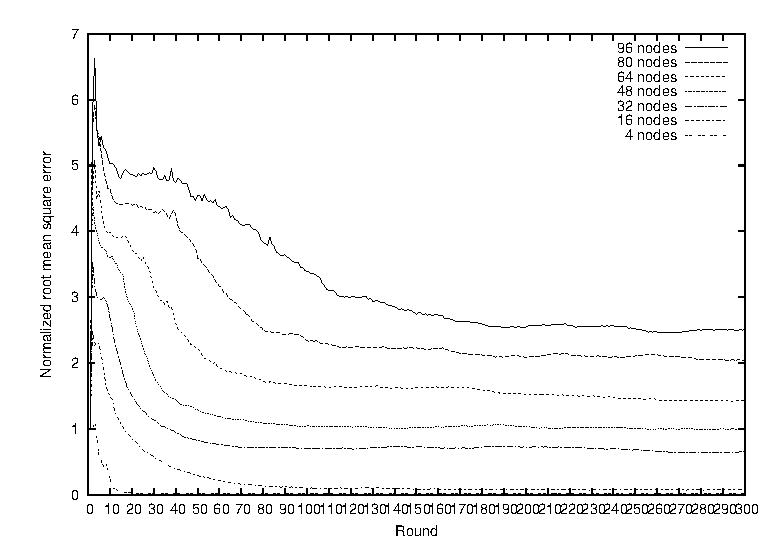
\includegraphics[width=2.5in]{figure/desync-0-75}%
	\label{fig:alpha075}}
    \hspace{8pt}%
	\subfloat[$\alpha$ = 0.80]{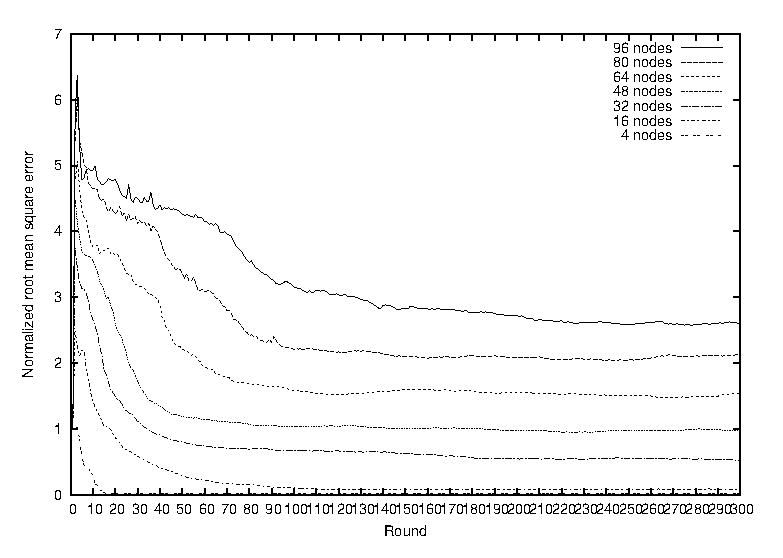
\includegraphics[width=2.5in]{figure/desync-0-80}%
	\label{fig:alpha080}}
	\subfloat[$\alpha$ = 0.85]{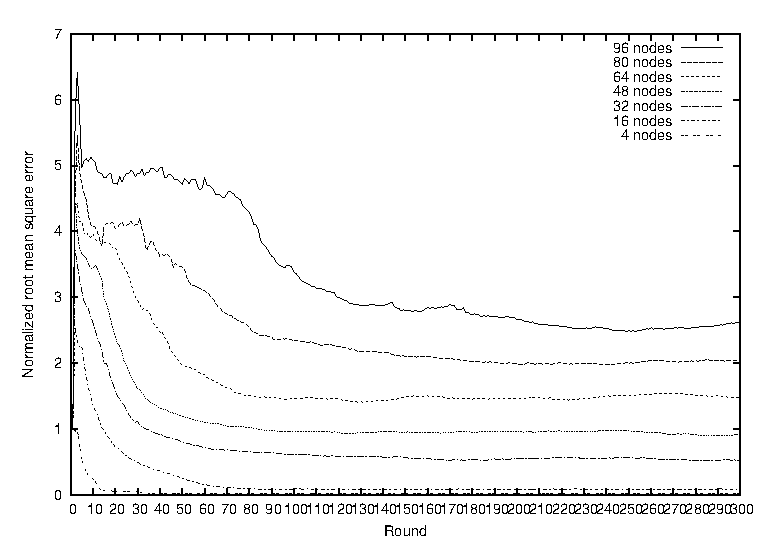
\includegraphics[width=2.5in]{figure/desync-0-85}%
	\label{fig:alpha085}}
    \hspace{8pt}%
	\subfloat[$\alpha$ = 0.90]{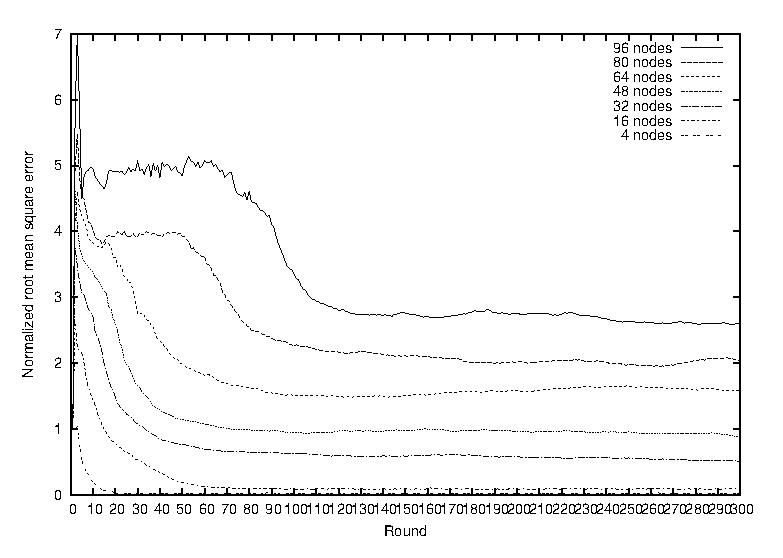
\includegraphics[width=2.5in]{figure/desync-0-90}%
	\label{fig:alpha090}}
	\subfloat[$\alpha$ = 0.95]{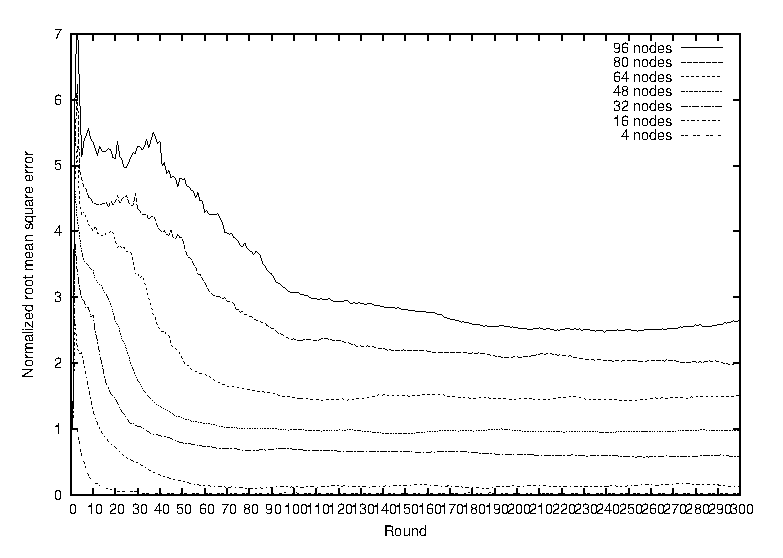
\includegraphics[width=2.5in]{figure/desync-0-95}%
	\label{fig:alpha095}}
\caption{DESYNC: Varying step size from 0.70 to 0.95}%
\label{fig:desync-vary-large}%
\lofcont
\end{figure*}

The result indicates that too small step size (0.10 to 0.35) leads to slow convergence speed and high error.
Increasing step size tends to lead to lower error. Step sizes from 0.65 to 0.95 do not result in much different in term of error but the larger value tends to lead to faster convergence speed.
However, increasing step size from 0.80 to 0.95 does not significantly improve the performance. Therefore, we can use 0.95  which is the same value used in \cite{4379660} as the step size for DESYNC to compare with DWARF.

\subsection{Desynchronization Error}
\label{sec:error}
To measure the desynchronization error, we run the simulation for 300 time periods. 
In each network size, we run the simulation for 30 times.
Then, we measure the average root mean square error (RMSE). The error (ERR) is the measured phase difference minus the perfect phase difference:

\begin{equation}
ERR_i = \Delta \phi_{i,j} - T/n, \nonumber
\end{equation}
\begin{equation}
RMSE = \sqrt{\frac{\sum_{i = 1}^{n}{ERR_i^2}}{n}}, \nonumber
\end{equation}
where node $j$ is the next phase neighbor of node $i$.
$\Delta \phi_{i,j}$ is the phase difference between node $i$ and node $j$ on the time period $T$.
Given that $n$ is a total number of nodes, $T/n$ is the perfect phase difference.

%Figure \ref{fig:rmse300rounds} illustrates the result of the desynchronization error in each network size after 300 time periods.
However, a smaller absolute error in a dense network is not necessarily better than a bigger error in a sparse network because the perfect phase difference in a dense network is also smaller than that in a sparse network.
Thus, for a comparable view of each network size, we also measure a normalized root mean square error (NRMSE) that is a ratio of the root mean square error and the perfect phase difference of each network size.
% (see Figure \ref{fig:nrmse300rounds}).
Figure  \ref{fig:rmse300rounds} illustrate the result of absolute desynchronization error and Figure \ref{fig:nrmse300rounds} illustrates the result of the normalized desynchronization error in each network size after 300 time periods.

\begin{figure}[!t]
\centering
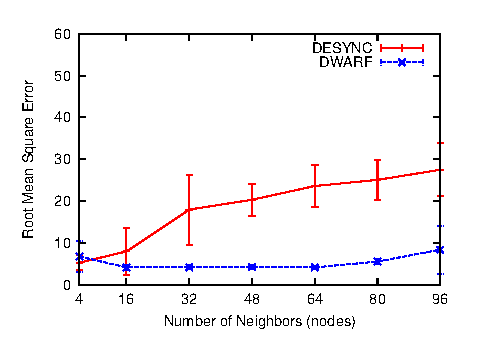
\includegraphics[width=3.0in]{figure/compare300rounds_rmse_sd}
\caption{Root mean square error after 300 time periods}
\label{fig:rmse300rounds}
\end{figure}

\begin{figure}[!t]
\centering
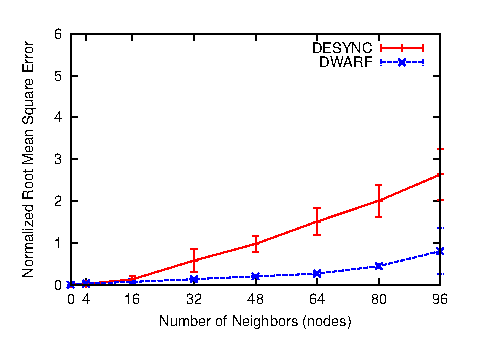
\includegraphics[width=3.0in]{figure/compare300rounds_nrmse-expected_sd}
\caption{Root mean square error normalized by perfect phase difference after 300 time periods}
\label{fig:nrmse300rounds}
\end{figure}

The result indicates that, in all network sizes (4 - 96 nodes), DWARF achieves significantly better  desynchrony states than DESYNC does.
Understandably, using information from all neighbors (as in DWARF) leads to lower errors than using information from only two phase neighbors (as in DESYNC) does. Furthermore, DESYNC's mechanism allows a phase error of a node to propagate to its phase neighbors. A part of this error will propagate back and forth between two phase neighbors as well as circulate inside the network. As a result, DESYNC's error after convergence is still quite large.
In contrast, DWARF is robust to this error propagation. Even though the error propagation may still occur, the impact is not significant. Given that DWARF uses the sum of forces from all neighbors, an error from one neighbor does not overwhelm the system.

We note that we show RMSE and NRMSE after 300 periods because, by that time, the errors of all simulation scenarios seem to be stable. The actual convergence time in most scenarios is much lower than 300 rounds (see the next section).

\subsection{Convergence Time}
\label{sec:converge}
In the desynchronization error evaluation, we only measure the performance after 300 time periods.
However, the previous result does not indicate whether the protocols have converged or not.
Neither does it indicate how fast the protocols have converged. 
Hence, we also measure the absolute root mean square error and normalized root mean square error for each time period.

In sparse networks (Figure \ref{fig:rmse-sparse} and \ref{fig:nrmse-sparse}), both protocols converge with similar small error but DWARF converges slightly faster. 
In dense networks (Figure \ref{fig:rmse-dense} and \ref{fig:nrmse-dense}) and extremely dense networks (Figure \ref{fig:rmse-extreme} and \ref{fig:nrmse-extreme}), both protocols still converge.
Even though DESYNC converges faster in such networks, it converges with a relatively high error compared to that of DWARF.
In addition, at the time when DESYNC has converged and DWARF has not converged yet, DWARF's error is already lower than DESYNC's.
Furthermore, in dense and extremely dense networks, the normalized root mean square errors of DESYNC after convergence is higher or equal to 1.
This means that the error is very large compared to the perfect phase difference.
Conversely, the normalized error of DWARF is lower than 1 even in the extremely dense networks.
Therefore, DWARF scales well with the network density whereas DESYNC does not.

In a denser network, the errors of DESYNC and DWARF are higher because the probability of message collisions increases (see the next section). 


\begin{figure*}[!t]
\centerline{
	\subfloat[Sparse]{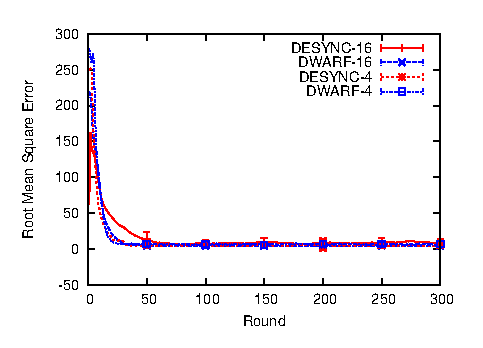
\includegraphics[width=2.0in]{figure/compare-rmse-4-16nodes_sd}%
	\label{fig:rmse-sparse}}
	\hfil
	\subfloat[Dense]{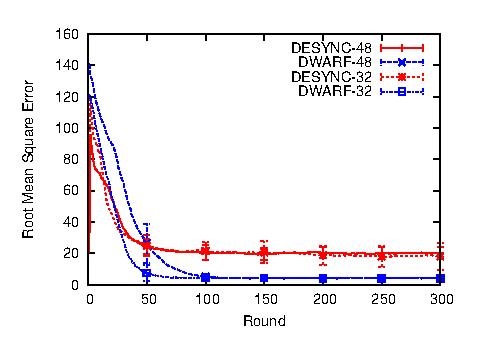
\includegraphics[width=2.0in]{figure/compare-rmse-32-48nodes_sd}%
	\label{fig:rmse-dense}}
	\hfil
	\subfloat[Extremely Dense]{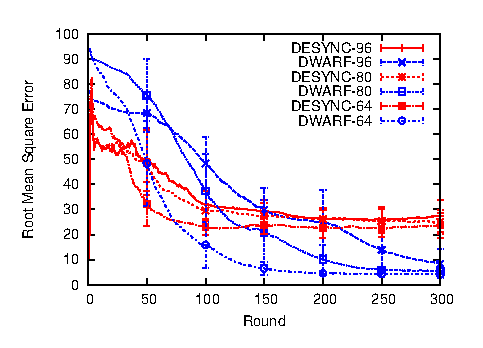
\includegraphics[width=2.0in]{figure/compare-rmse-64-80-96nodes_sd}%
	\label{fig:rmse-extreme}}
}
\caption{Convergence time and absolute root mean square error}
\label{fig:rmse-convergence}
\lofcont
\end{figure*}

\begin{figure*}[!t]
\centerline{
	\subfloat[Sparse]{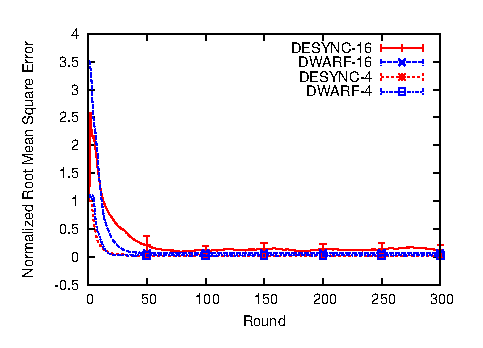
\includegraphics[width=2.0in]{figure/compare-nrmse-4-16nodes_sd}%
	\label{fig:nrmse-sparse}}
	\hfil
	\subfloat[Dense]{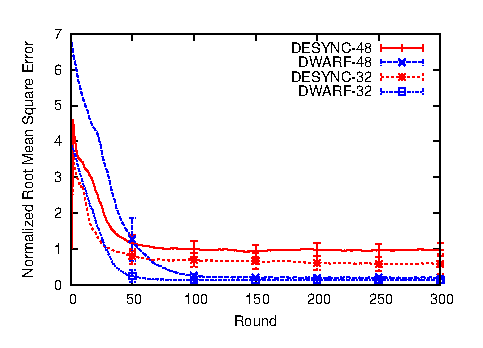
\includegraphics[width=2.0in]{figure/compare-nrmse-32-48nodes_sd}%
	\label{fig:nrmse-dense}}
	\hfil
	\subfloat[Extremely Dense]{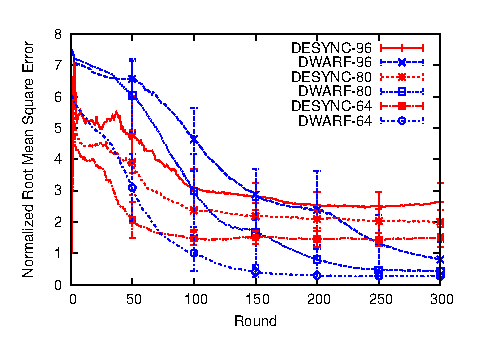
\includegraphics[width=2.0in]{figure/compare-nrmse-64-80-96nodes_sd}%
	\label{fig:nrmse-extreme}}
}
\caption{Convergence time and root mean square error normalized by expected phase difference}
\label{fig:nrmse-convergence}
\lofcont
\end{figure*}

\subsection{Correlation of Packet Loss and Desynchronization Error }
In this section, we investigate the correlation of packet loss and desynchronization error. 
We only include the results of DWARF in networks of 16, 48, and 80 nodes for 300 time periods (Figure \ref{fig:error-loss}). 
However, in networks of 4, 32, 64, and 96 nodes, the results are similar (not shown).

At the beginning, the network is far from the perfect desynchrony state and messages from different nodes are simultaneously fired. 
This results in lost packets and errors.
However, over time, nodes gradually adapt their time phases. 
Consequently, the number of lost packets and the error also gradually drop.


\begin{figure*}[!t]
\centerline{
	\subfloat[16 nodes]{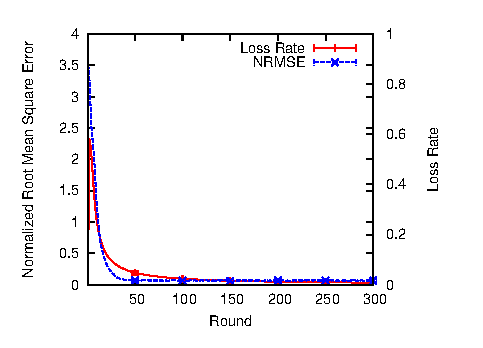
\includegraphics[width=2.2in]{figure/error-loss-16nodes_sd}%
	\label{fig:error-loss-16nodes}}
	\hfil
	\subfloat[48 nodes]{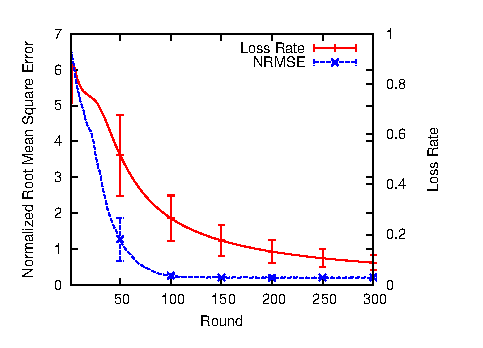
\includegraphics[width=2.2in]{figure/error-loss-48nodes_sd}%
	\label{fig:error-loss-48nodes}}
	\hfil
	\subfloat[80 nodes]{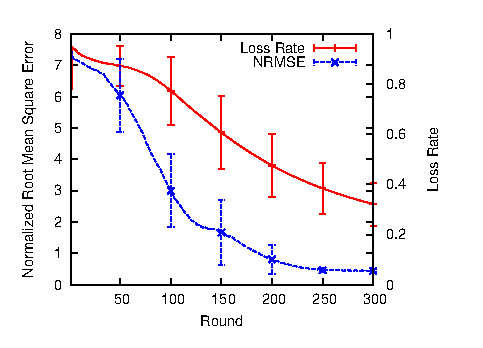
\includegraphics[width=2.2in]{figure/error-loss-80nodes_sd}%
	\label{fig:error-loss-80nodes}}
}
\caption{Correlation of packet loss and desynchronization error}
\label{fig:error-loss}
\lofcont
\end{figure*}
\section{Summary}
In this chapter, we present DWARF, a novel desynchronization algorithm that enables nodes in a system to perform tasks at different time. To the best of our knowledge, DWARF is the first desynchronization algorithm that is based on the concept of electromagnetic fields, a foundation of physics.
Our algorithm is completely distributed and localized with no reliance on a centralized node or a global notion of time. Due to low complexity in terms of computation, memory, and message overhead, DWARF is suitable for traditional wireless networks as well as resource-constraint wireless sensor networks. Our result indicates that DWARF can significantly outperform DESYNC by reducing 10 - 63\% of the desynchronization error. In addition, DWARF scales well with network size given that the normalized error is lower than 1 even in extremely dense networks.

The evaluation result of DWARF is promising. This result indicates that physicomimetics approach is viable for desynchronization. However, the evaluation has been performed on single-hop networks. Typically, wireless sensor networks are multi-hop networks. There are several issues to be concerned in extending DWARF to such networks. We cover such issues and present the multi-hop extension of DWARF in Chapter \ref{chap:multihop}.
Additionally, the evaluation does not show the mathematical evidence that the algorithm is stable and does not indicate why the algorithm converges. Therefore, we analyses the stability of the algorithm in the next chapter.




\chapter{Convexity and Stability Analysis of the Single-hop Algorithm}
\label{chap:stability-singlehop}
In the previous chapter, we present DWARF, a physicomimetics desynchronization algorithm. From the evaluation results, the algorithm is eventually stable with low desynchronization error. 
However, it is not obvious that why DWARF is eventually stable with low error. 
Therefore, in this chapter, we mathematically analyse the stability of the algorithm.

We divide our analysis into two parts. First, we analyse the convexity of the force function. If the force function is convex, the system contains one global minima and no local minima. Therefore, the system could reach the perfect desynchrony state by gradually reducing the overall force of the system. Second, we analyse the stability when the system at the equilibrium. If the system is stable, it can be back to the equilibrium under a small perturbation. 

\section{Convexity Analysis}
\label{sec:convex}
In this section, our goal is to prove that the force function used in DWARF has one global minima and no local minima. In other words, we will prove that the force function is convex.

Let $F_{i}$ be the force summation at node $i$ and $\Delta_{i,j} \in (-\frac{T}{2}, \frac{T}{2})$  is an interval between node $i$ and $j$.
If $\Delta_{i,j} > 0$, the node $j$ repels the node $i$ in a positive direction.
In contrast,  if $\Delta_{i,j} < 0$, the node $j$ repels the node $i$ in a negative direction.

Therefore, for $n$ nodes, $F_{i}$ can be formulated as the following equation, 
\begin{equation}
F_{i} = \sum_{\substack{j=1\\j \neq i}}^{n} \frac{1}{\Delta_{i,j}}.
\end{equation}

The objective function $E$ of the system is the summation of absolute received forces at all nodes,
\begin{equation}
E = \sum_{i = 1}^{n}\left| F_{i} \right| = \sum_{i = 1}^{n} \left | \sum_{\substack{j=1\\j \neq i}}^{n} \frac{1}{\Delta_{i,j}} \right| 
\label{eq:energy}
\end{equation}
To prove the function $E$ is a convex function, we must prove that two following conditions are satisfied; 1) the set of all $\Delta_{i,j}$ is a convex set and 2) the Hessian matrix of $E$ is positive semidefinite. 

\begin{prop}
A set of all possible interval $\Delta_{i,j}$ is a convex set.
\label{prop:convexset}
\end{prop}
\begin{proof}
A set of $(-\frac{T}{2}, \frac{T}{2})$ is a line connecting between $-\frac{T}{2}$ and $\frac{T}{2}$. 
Therefore, any $\Delta_{i_1,j_1}$, $\Delta_{i_2,j_2} \in$  $(-\frac{T}{2}, \frac{T}{2})$ and $\alpha \in \mathbb{R}$ with $0 \le \alpha \le 1$,
\begin{equation}
\alpha\Delta_{i_1,j_1} + (1-\alpha)\Delta_{i_2,j_2} \in (-\frac{T}{2}, \frac{T}{2}). \nonumber
\end{equation} 
\end{proof}

\begin{prop}
The Hessian of the function $E$ is positive semidefinite.
\label{prop:Hessian}
\end{prop}

\begin{proof}
Let $H$ be the Hessian matrix of the objective function $E$,

$H = 
\begin{pmatrix} 
{\frac{\partial^2 E}{\partial \Delta_{1,2}^2}}  & {\frac{\partial^2 E}{\partial \Delta_{1,2}\partial\Delta_{1,3}}}  & \cdots & {\frac{\partial^2 E}{\partial \Delta_{1,2}\partial \Delta_{n,n-1}}} \\ 
{\frac{\partial^2 E}{\partial \Delta_{1,3}\partial \Delta_{1,2}}}  & {\frac{\partial^2 E}{\partial \Delta_{1,3}^2}} & \cdots & {\frac{\partial^2 E}{\partial \Delta_{1,3}\partial \Delta_{n,n-1}}} \\ 
\vdots & \vdots & \ddots & \vdots \\
{\frac{\partial^2 E}{\partial \Delta_{n,n-1}\partial \Delta_{1,2}}} & {\frac{\partial^2 E}{\partial \Delta_{n,n-1}\partial \Delta_{1,3}}} & \cdots & {\frac{\partial^2 E}{\partial \Delta_{n,n-1}^2}}
\end{pmatrix}$.

For any $\Delta_{x,y}$, we derive the first-order derivative as follows,
\begin{equation}
{\frac{\partial E}{\partial \Delta_{x,y}}} = \frac{\sum_{\substack{j=1\\j \neq x}}^{n} \frac{1}{\Delta_{x,j}} }{\left| \sum_{\substack{j=1\\j \neq x}}^{n} \frac{1}{\Delta_{x,j}} \right|} \left( - \frac{1}{\Delta_{x,y}^2} \right). \nonumber
\end{equation}

For the second-order partial derivatives, if we differentiate with the same $\Delta_{x,y}$, 
\begin{alignat}{2}
{\frac{\partial^2 E}{\partial \Delta_{x,y}^2}} = \frac{\sum_{\substack{j=1\\j \neq x}}^{n} \frac{1}{\Delta_{x,j}} }{\left| \sum_{\substack{j=1\\j \neq x}}^{n} \frac{1}{\Delta_{x,j}} \right|} \left( \frac{2}{\Delta_{x,y}^3} \right). \nonumber
\end{alignat}

In the other hand, if we differentiate with other $\Delta_{u,v}$, where $u \neq x$ or $v \neq y$, ${\frac{\partial^2}{\partial \Delta_{u,v}\partial\Delta_{x,y}}}E = 0$.

Therefore, the Hessian matrix of the function $E$ is

$H = 
\begin{pmatrix} 
a_{1,2} & 0 & \cdots & 0 \\ 
0 & a_{1,3} & \cdots & 0 \\ 
\vdots & \vdots & \ddots & \vdots \\
0 & 0 & \cdots & a_{n, n-1} \\ 
\end{pmatrix}$,

where $a_{i,j} = \frac{u_{i}}{|u_{i}|} \left( \frac{2}{\Delta_{i,j}^3} \right)$ and $u_{i} = \sum_{\substack{j=1\\j \neq i}}^{n}  \frac{1}{\Delta_{i,j}}$.

To show that the Hessian matrix of the function $E$ is positive semidefinite, we show that $\vec{\Delta}^{T}H\vec{\Delta} \geq 0$ for all $\vec{\Delta}$ when $\vec{\Delta} \neq 0$.

\begin{alignat}{2}
\vec{\Delta}^{T}H\vec{\Delta} &=
\begin{pmatrix}
 \Delta_{1,2} & \Delta_{1,3} & \cdots & \Delta_{n,n-1} \\
\end{pmatrix}
H
\begin{pmatrix}
 \Delta_{1,2} \\
 \Delta_{1,3} \\
 \vdots \\
 \Delta_{n,n-1}
\end{pmatrix} \nonumber \\
=& \text{ } \sum_{i = 1}^{n} \sum_{\substack{j=1\\j \neq i}}^{n} \frac{u_{i}}{|u_{i}|}  \left( \frac{2}{\Delta_{i,j}} \right) \nonumber \\
=& \text{ } 2 \sum_{i = 1}^{n} \frac{u_{i}}{|u_{i}|} \sum_{\substack{j=1\\j \neq i}}^{n}  \frac{1}{\Delta_{i,j}} \nonumber \\
=& \text{ } 2 \sum_{i = 1}^{n} \frac{u_{i}}{|u_{i}|} u_{i} = 2 \sum_{i = 1}^{n} |u_{i}| \nonumber \\
\geq& \text{ } 0 \nonumber
\end{alignat}

Therefore, we conclude that $\vec{\Delta}^{T}H\vec{\Delta} \geq 0$ and the Hessian matrix of $E$ is positive semidefinite.  
\end{proof}

From Proposition \ref{prop:convexset} and \ref{prop:Hessian}, we derive the following lemma.
\begin{lem}
the function $E$ is a convex function.
\label{lemma:convexset}
\end{lem}

From the above lemma, we finish our proof with the following theorem.

\begin{thm}
The system force summation function of DWARF has one global minima and no local minima.
\label{theorem:minima}
\end{thm}

\section{Stability Analysis}
\label{sec:stability}
To prove that the system is stable, we begin by transforming the system into a non-linear dynamic system. 
The evenness of the number of nodes affects the analysis. Therefore, we divide the non-linear dynamic system into two cases: when $n$ is even and when $n$ is odd where $n$ is the number of nodes.

1) when $n$ is even: Figure \ref{fig:even-perfect} illustrates the equilibrium of a dynamic system when the number of nodes is even. Noticeably, node 0 and $n/2$ are exactly at the opposite side of each other. At the first snapshot of the system, node 0 adjusts its phase based on the force function of DWARF. After adjustment, we re-label node 1 to 0, node 2 to 1, ..., node $n-1$ to $n-2$, and node 0 to $n-1$ for analysis at the next snapshot (see Figure \ref{fig:even-adapt}).
Therefore, to transform into a difference equation, $\Delta_{1}$ in the next snapshot is $\Delta_{2}$ in the previous snapshot, $\Delta_{2}$ in the next snapshot is $\Delta_{3}$ in the previous snapshot, and so on. However, $\Delta_{n-1}$ and $\Delta_{n}$ in the next snapshot are $\Delta_{n}$ and $\Delta_{1}$ in the previous snapshot adjusted by the force function, respectively.
\begin{figure*}[!t]
\centerline{
	\subfloat[]{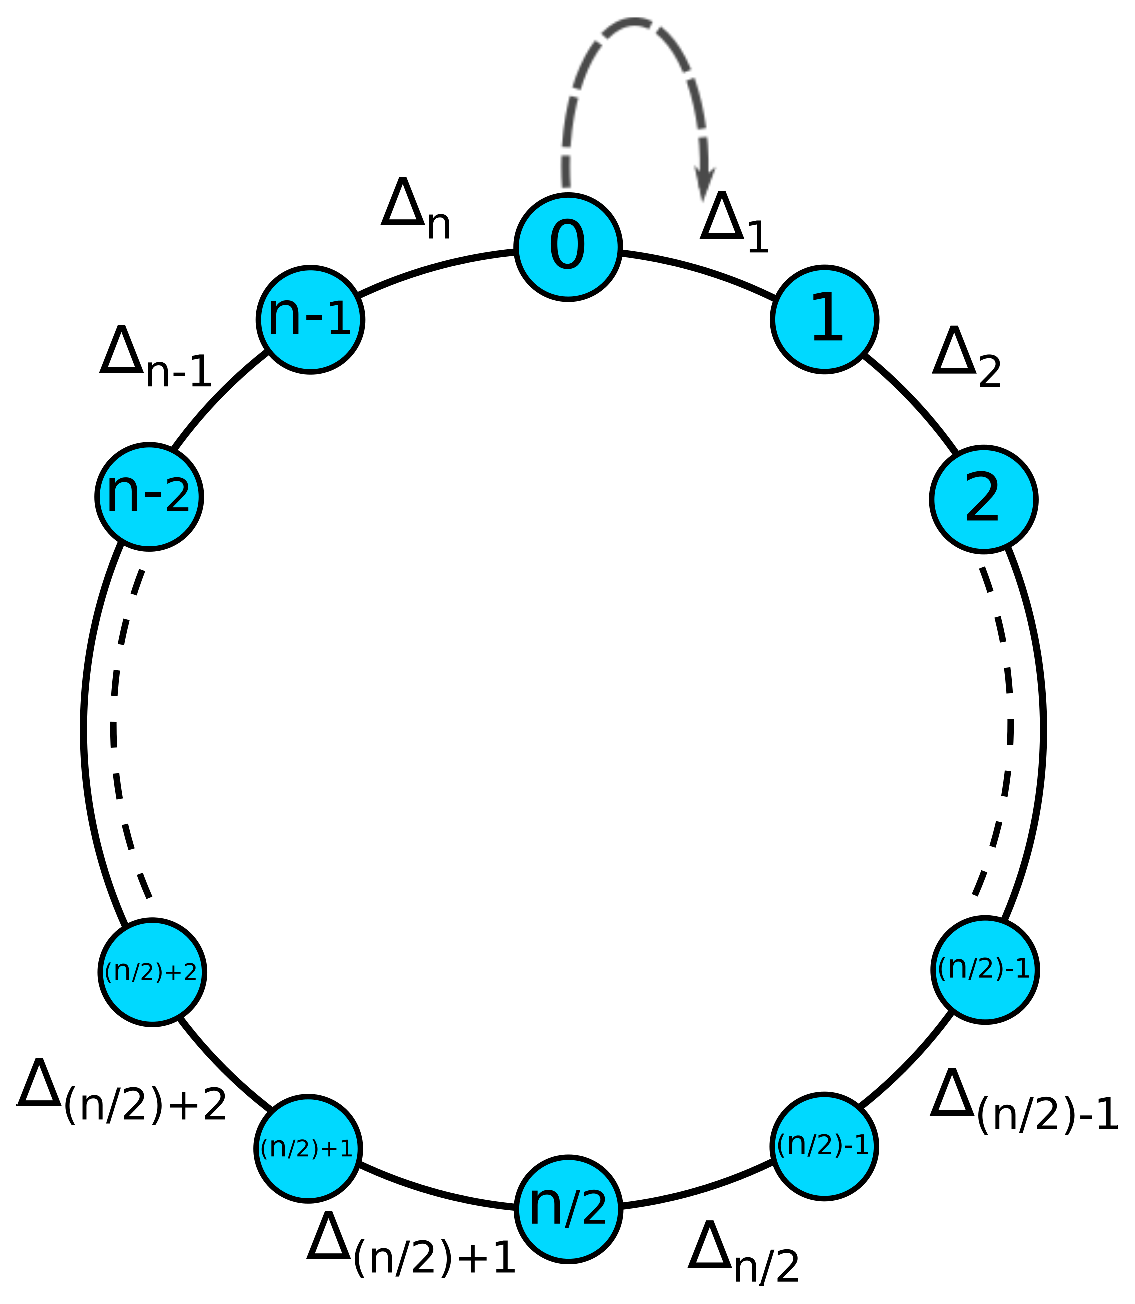
\includegraphics[scale=0.30]{figure/stability-onehop-even}%
	\label{fig:even-perfect}}
	\hfil
	\subfloat[]{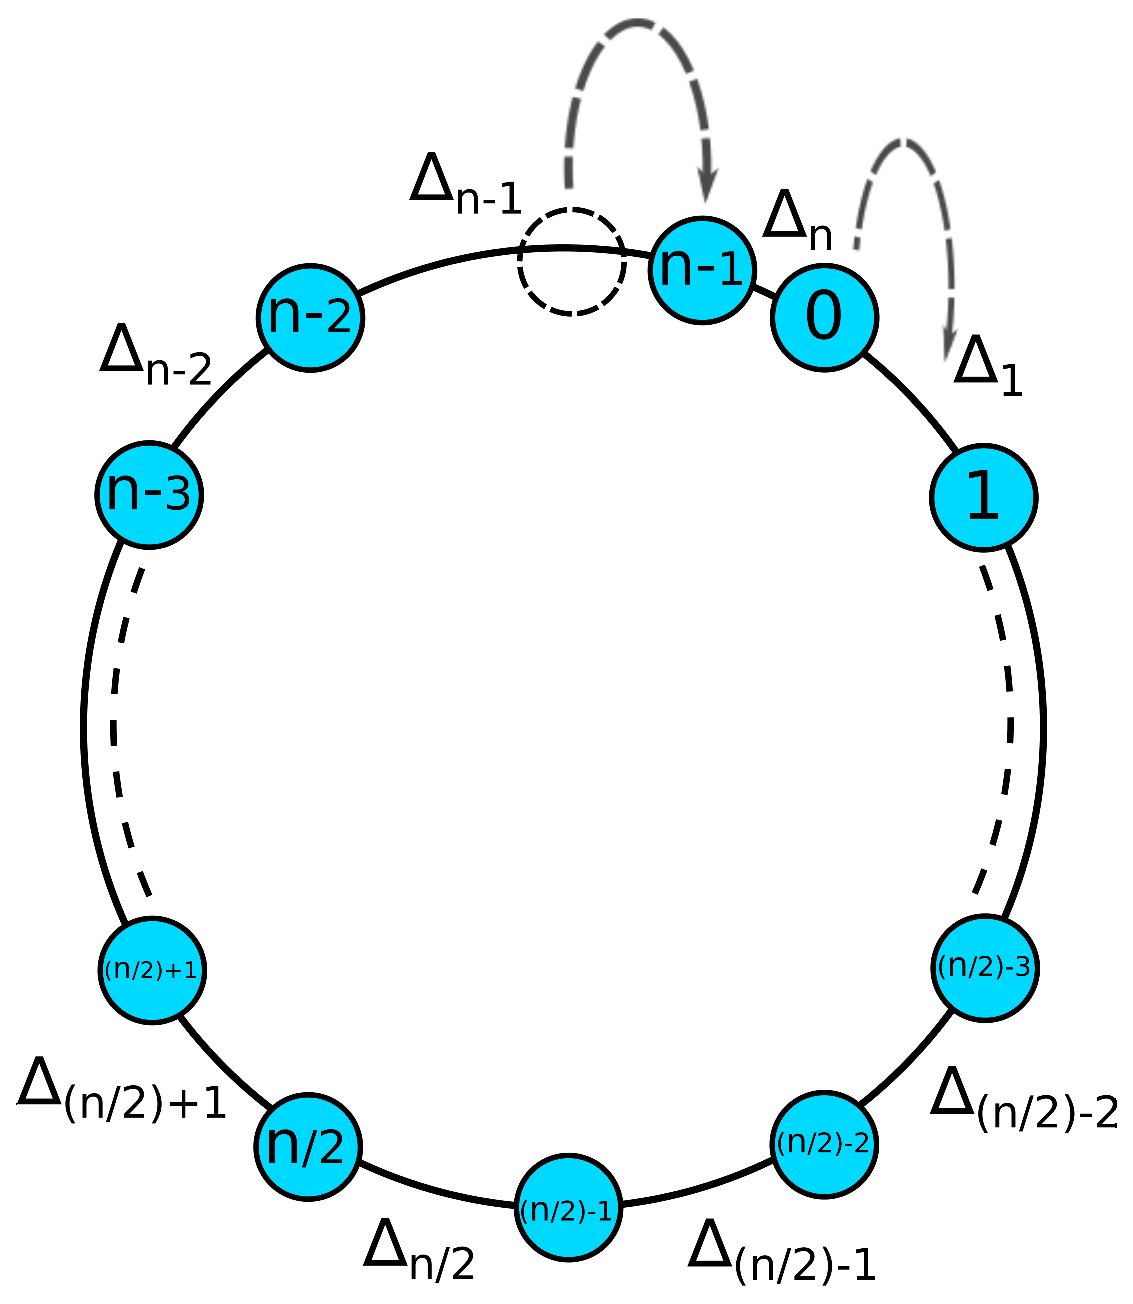
\includegraphics[scale=0.30]{figure/stability-onehop-even-adapt}%
	\label{fig:even-adapt}}
}
\caption{Non-linear dynamic system when $n$ is even. (a) The snapshot of the system at one time step. (b) In next time step after node 0 adjusts its phase, node 1 in previous round is re-labelled to 0, node 2 is re-labelled to 1, and so on.}
\label{fig:n-even}
\lofcont
\end{figure*}
Therefore, the non-linear dynamic system when $n$ is even can be expressed as the following difference equations:

\begin{alignat}{1}
 \Delta_{1} =& \Delta_{2} \nonumber \\
 \Delta_{2} =& \Delta_{3} \nonumber \\
 \vdots \nonumber \\
 \Delta_{n-2} =& \Delta_{n-1} \nonumber \\
 \Delta_{n-1} =& \Delta_{n} + KT\Bigg( -\frac{1}{\Delta_{1}} - \frac{1}{\Delta_{1} + \Delta_{2}} - \hdots - \frac{1}{\Delta_{1} + \Delta_{2} + \hdots + \Delta_{\frac{n}{2}-1}} \nonumber \\ 
&+ \frac{1}{\Delta_{n}} + \frac{1}{\Delta_{n} + \Delta_{n-1}} + \hdots + \frac{1}{\Delta_{n} + \Delta_{n-1} + \hdots + \Delta_{\frac{n}{2}+2}}\Bigg) \nonumber \\
 \Delta_{n} =& \Delta_{1} - KT\Bigg( -\frac{1}{\Delta_{1}} - \frac{1}{\Delta_{1} + \Delta_{2}} - \hdots - \frac{1}{\Delta_{1} + \Delta_{2} + \hdots + \Delta_{\frac{n}{2}-1}} \nonumber \\ 
&+ \frac{1}{\Delta_{n}} + \frac{1}{\Delta_{n} + \Delta_{n-1}} + \hdots + \frac{1}{\Delta_{n} + \Delta_{n-1} + \hdots + \Delta_{\frac{n}{2}+2}}\Bigg) 
\end{alignat}

We note that the force from node $n/2$ in the previous snapshot is already balanced when we consider node 0. Therefore, $\Delta_{\frac{n}{2}}$ and $\Delta_{\frac{n}{2}+1}$ do not appear in the force equation for adjusting $\Delta_{n-1}$ and $\Delta_{n}$ in the next snapshot.

2) when $n$ is odd:
Similarly, Figure \ref{fig:n-odd} illustrates the non-linear dynamic system when $n$ is odd. The only difference from when $n$ is even is that there is no node that is opposite to node 0. Therefore, in the difference equations, only $\Delta_{\lceil\frac{n}{2}\rceil}$ from the previous snapshot does not appear in the force equation for adjusting $\Delta_{n-1}$ and $\Delta_{n}$ in the next snapshot.
\begin{figure*}[!t]
\centerline{
	\subfloat[]{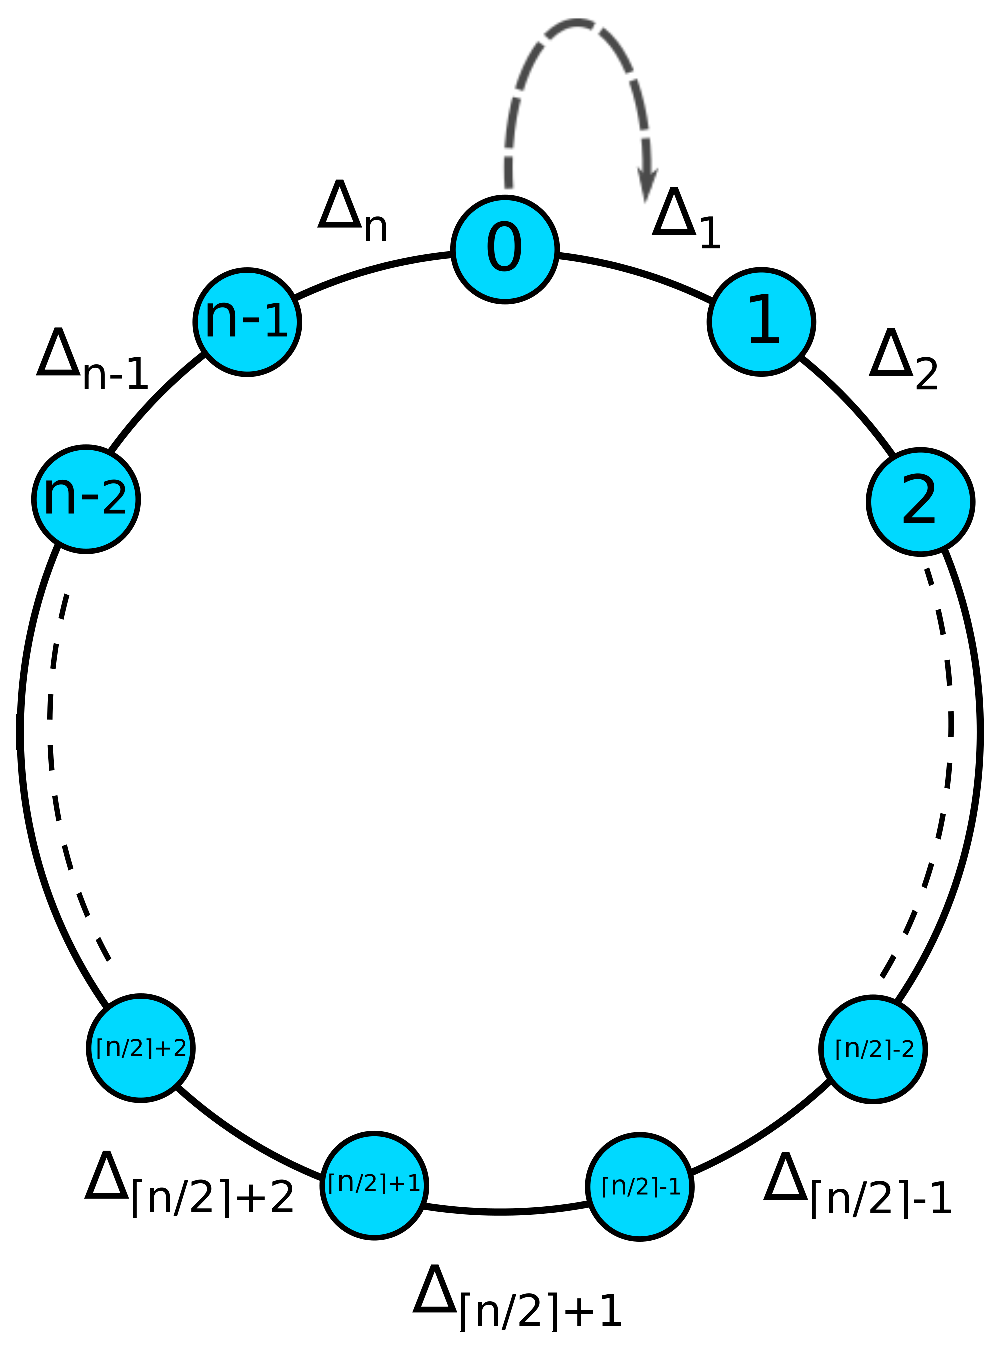
\includegraphics[scale=0.30]{figure/stability-onehop-odd}%
	\label{fig:odd}}
	\hfil
	\subfloat[]{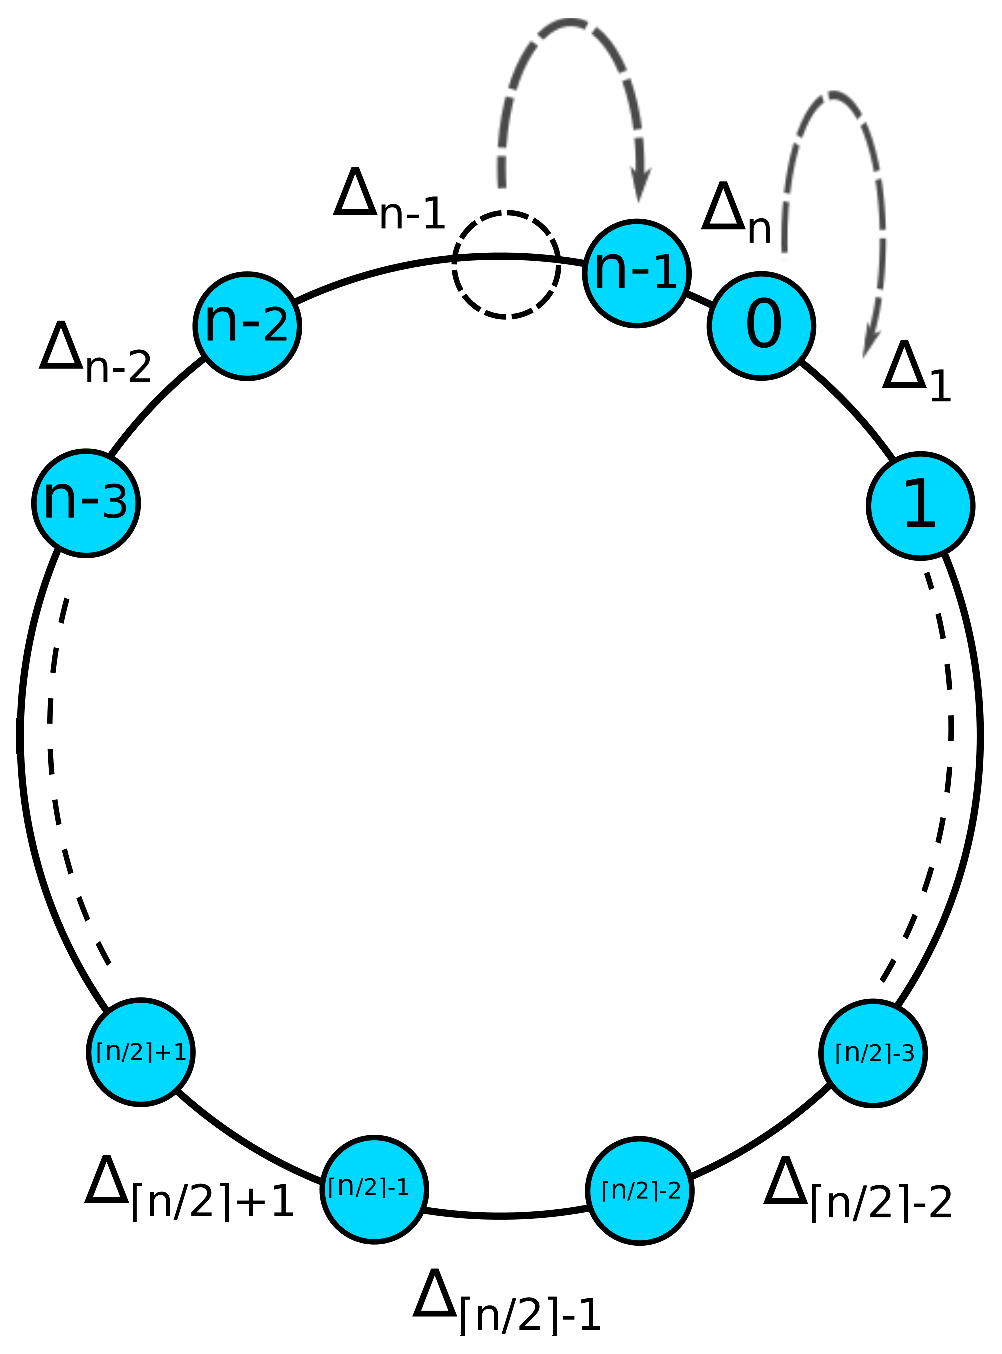
\includegraphics[scale=0.30]{figure/stability-onehop-odd-adapt}%
	\label{fig:odd-adapt}}
}
\caption{Non-linear dynamic system when $n$ is odd. (a) The snapshot of the system at one time step. (b) In next time step after node 0 adjusts its phase, node 1 in previous round is re-labelled to 0, node 2 is re-labelled to 1, and so on.}
\label{fig:n-odd}
\lofcont
\end{figure*}
\begin{alignat}{1}
 \Delta_{1} =& \Delta_{2} \nonumber \\
 \Delta_{2} =& \Delta_{3} \nonumber \\
 \vdots \nonumber \\
 \Delta_{n-2} =& \Delta_{n-1} \nonumber \\
 \Delta_{n-1} =& \Delta_{n} + KT\Bigg( -\frac{1}{\Delta_{1}} - \frac{1}{\Delta_{1} + \Delta_{2}} - \hdots - \frac{1}{\Delta_{1} + \Delta_{2} + \hdots + \Delta_{\lceil{\frac{n}{2}}\rceil-1}} \nonumber \\ 
&+ \frac{1}{\Delta_{n}} + \frac{1}{\Delta_{n} + \Delta_{n-1}} + \hdots + \frac{1}{\Delta_{n} + \Delta_{n-1} + \hdots + \Delta_{\lceil\frac{n}{2}\rceil+1}}\Bigg) \nonumber \\
 \Delta_{n} =& \Delta_{1} - KT\Bigg( -\frac{1}{\Delta_{1}} - \frac{1}{\Delta_{1} + \Delta_{2}} - \hdots - \frac{1}{\Delta_{1} + \Delta_{2} + \hdots + \Delta_{\lceil\frac{n}{2}\rceil-1}} \nonumber \\ 
&+ \frac{1}{\Delta_{n}} + \frac{1}{\Delta_{n} + \Delta_{n-1}} + \hdots + \frac{1}{\Delta_{n} + \Delta_{n-1} + \hdots + \Delta_{\lceil\frac{n}{2}\rceil+1}}\Bigg) \nonumber 
\end{alignat}

Due to the non-linear adaptation function, the standard linear dynamic system analysis does not suffice.
Therefore, we locally analyse stability of the system around a fixed point which is the equilibrium point.
We begin by linear approximation to find the Jacobian at the equilibrium. Then, from the Jacobian, we find the bound of eigenvalues which is the crucial part of stability analysis.


\subsection{Linear Approximation}
The Jacobian ($J$) of a difference equations system is defined as follows:

\begin{alignat}{2}
J=\begin{pmatrix} 
{\frac{\partial \Delta_{1}}{\partial \Delta_{1}}}  & {\frac{\partial \Delta_{1}}{\partial \Delta_{2}}} & \cdots & {\frac{\partial \Delta_{1}}{\partial \Delta_{n-1}}} & {\frac{\partial \Delta_{1}}{\partial \Delta_{n}}} \\ 
{\frac{\partial \Delta_{2}}{\partial \Delta_{1}}}  & {\frac{\partial \Delta_{2}}{\partial \Delta_{2}}} & \cdots &  {\frac{\partial \Delta_{2}}{\partial \Delta_{n-1}}} & {\frac{\partial \Delta_{2}}{\partial \Delta_{n}}} \\  
\vdots & \vdots & \ddots & \vdots & \vdots \\
{\frac{\partial \Delta_{n-1}}{\partial \Delta_{1}}} & {\frac{\partial \Delta_{n-1}}{\partial \Delta_{2}}} & \cdots &  {\frac{\partial \Delta_{n-1}}{\partial \Delta_{n-1}}} & {\frac{\partial \Delta_{n-1}}{\partial \Delta_{n}}} \\  
{\frac{\partial \Delta_{n}}{\partial \Delta_{1}}} & {\frac{\partial \Delta_{n}}{\partial \Delta_{2}}} & \cdots &  {\frac{\partial \Delta_{n}}{\partial \Delta_{n-1}}} & {\frac{\partial \Delta_{n}}{\partial \Delta_{n}}} \\  
\end{pmatrix}
\end{alignat}

We consider the Jacobian when $n$ is even and odd separately. In both cases, after finding the Jacobian, we substitute each $\Delta_{i}$ with $T/n$ which is the phase interval between each node at the equilibrium.

1) $n$ is even:

For $\Delta_{i}, 1 \leq i \leq n-2$, partial derivatives of ${\partial \Delta_{i} / \partial \Delta_{j}}, 1 \leq j \leq n$ are the followings:
\begin{alignat}{1}
  {\frac{\partial \Delta_{i}}{\partial \Delta_{j}}} = \left\{ 
  \begin{array}{l l}
    1 & \quad \text{if } j = i + 1\\
    0 & \quad \text{otherwise}\\
  \end{array} \right. \nonumber
\end{alignat}


For $\Delta_{n-1}$, we find its partial derivatives as follows:
\begin{alignat}{1}
{\frac{\partial \Delta_{n-1}}{\partial \Delta_{1}}} =& KT\left(\frac{1}{\Delta_1^2} + \frac{1}{(\Delta_1 + \Delta_2)^2} + \cdots + \frac{1}{(\Delta_1 + \Delta_2 + \cdots + \Delta_{\frac{n}{2}-1})^2}\right) \nonumber \\
=&KT\left(\frac{n^2}{T^2}\right)\left(\frac{1}{1^2} + \frac{1}{2^2} + \cdots + \frac{1}{(\frac{n}{2}-1)^2}\right) = \frac{Kn^2}{T} \sum\limits_{i=1}^{\frac{n}{2}-1}{\frac{1}{i^2}} \nonumber \\
{\frac{\partial \Delta_{n-1}}{\partial \Delta_{2}}} =& KT\left(\frac{1}{(\Delta_1 + \Delta_2)^2} + \cdots + \frac{1}{(\Delta_1 + \Delta_2 + \cdots + \Delta_{\frac{n}{2}-1})^2}\right) \nonumber \\
=&KT\left(\frac{n^2}{T^2}\right)\left(\frac{1}{2^2} + \cdots + \frac{1}{(\frac{n}{2}-1)^2}\right) = \frac{Kn^2}{T} \sum\limits_{i=2}^{\frac{n}{2}-1}{\frac{1}{i^2}} \nonumber \\
\vdots \nonumber \\
{\frac{\partial \Delta_{n-1}}{\partial \Delta_{\frac{n}{2}-1}}} =& KT\left(\frac{1}{(\Delta_1 + \Delta_2 + \cdots + \Delta_{\frac{n}{2}-1})^2}\right) \nonumber \\
=&KT\left(\frac{n^2}{T^2}\right)\left(\frac{1}{(\frac{n}{2}-1)^2}\right) = \frac{Kn^2}{T} \sum\limits_{i=\frac{n}{2}-1}^{\frac{n}{2}-1}{\frac{1}{i^2}} \nonumber \\	
{\frac{\partial \Delta_{n-1}}{\partial \Delta_{\frac{n}{2}}}} =& 0 \nonumber \\
{\frac{\partial \Delta_{n-1}}{\partial \Delta_{\frac{n}{2}+1}}} =& 0 \nonumber \\
{\frac{\partial \Delta_{n-1}}{\partial \Delta_{\frac{n}{2}+2}}} =& KT\left(-\frac{1}{(\Delta_n + \Delta_{n-1} + \cdots + \Delta_{\frac{n}{2}+2})^2}\right) \nonumber \\
=&-KT\left(\frac{n^2}{T^2}\right)\left(\frac{1}{(\frac{n}{2}-1)^2}\right) = -\frac{Kn^2}{T} \sum\limits_{i=\frac{n}{2}-1}^{\frac{n}{2}-1}{\frac{1}{i^2}} \nonumber \\	
\vdots \nonumber \\
{\frac{\partial \Delta_{n-1}}{\partial \Delta_{n-1}}} =& KT\left(-\frac{1}{(\Delta_n + \Delta_{n-1})^2} - \cdots - \frac{1}{(\Delta_n + \Delta_{n-1} + \cdots + \Delta_{\frac{n}{2}+2})^2}\right) \nonumber \\
=&-KT\left(\frac{n^2}{T^2}\right)\left(\frac{1}{2^2} + \cdots + \frac{1}{(\frac{n}{2}-1)^2}\right) = -\frac{Kn^2}{T} \sum\limits_{i=2}^{\frac{n}{2}-1}{\frac{1}{i^2}} \nonumber \\
{\frac{\partial \Delta_{n-1}}{\partial \Delta_{n}}} =& 1+KT\left(-\frac{1}{\Delta_n^2} - \frac{1}{(\Delta_n + \Delta_{n-1})^2} - \cdots - \frac{1}{(\Delta_n + \Delta_{n-1} + \cdots + \Delta_{\frac{n}{2}+2})^2}\right) \nonumber  \\
=&1-KT\left(\frac{n^2}{T^2}\right)\left(\frac{1}{1^2} + \frac{1}{2^2} + \cdots + \frac{1}{(\frac{n}{2}-1)^2}\right) = 1-\frac{Kn^2}{T} \sum\limits_{i=1}^{\frac{n}{2}-1}{\frac{1}{i^2}} \nonumber 
\end{alignat}

For $\Delta_{n}$, we find its partial derivatives which is similar to $\Delta_{n-1}$ as follows.

\begin{alignat}{1}
{\frac{\partial \Delta_{n}}{\partial \Delta_{1}}} =& 1-\frac{Kn^2}{T} \sum\limits_{i=1}^{\frac{n}{2}-1}{\frac{1}{i^2}} \nonumber \\
{\frac{\partial \Delta_{n}}{\partial \Delta_{2}}} =& -\frac{Kn^2}{T} \sum\limits_{i=2}^{\frac{n}{2}-1}{\frac{1}{i^2}} \nonumber \\
\vdots \nonumber \\
{\frac{\partial \Delta_{n}}{\partial \Delta_{\frac{n}{2}-1}}} =& -\frac{Kn^2}{T} \sum\limits_{i=\frac{n}{2}-1}^{\frac{n}{2}-1}{\frac{1}{i^2}} \nonumber \\	
{\frac{\partial \Delta_{n}}{\partial \Delta_{\frac{n}{2}}}} =& 0 \nonumber \\
{\frac{\partial \Delta_{n}}{\partial \Delta_{\frac{n}{2}+1}}} =& 0 \nonumber \\
{\frac{\partial \Delta_{n}}{\partial \Delta_{\frac{n}{2}+2}}} =& \frac{Kn^2}{T} \sum\limits_{i=\frac{n}{2}-1}^{\frac{n}{2}-1}{\frac{1}{i^2}} \nonumber \\	
\vdots \nonumber \\
{\frac{\partial \Delta_{n}}{\partial \Delta_{n-1}}} =& \frac{Kn^2}{T} \sum\limits_{i=2}^{\frac{n}{2}-1}{\frac{1}{i^2}} \nonumber \\
{\frac{\partial \Delta_{n}}{\partial \Delta_{n}}} =& \frac{Kn^2}{T} \sum\limits_{i=1}^{\frac{n}{2}-1}{\frac{1}{i^2}} \nonumber 
\end{alignat}

Let $\sum\limits_{s}$ stands for $\sum\limits_{i=s}^{\frac{n}{2}-1}{\frac{1}{i^2}}$, where $s \in [1,\frac{n}{2}-1]$ and let $A = Kn^2/T$.
The Jacobian matrix of the system, when $n$ is even, is

\begin{alignat}{1}
J=\begin{pmatrix}
 0 & 1  & \cdots & 0 & 0 & 0 & 0 & \cdots & 0 & 0\\ 
 0 & 0  & \ddots & 0 & 0 & 0 & 0 & \cdots & 0 & 0\\  
\vdots & \vdots & \ddots & \ddots & \vdots & \vdots & \vdots & \ddots & \vdots & \vdots\\
 0 & 0  & \cdots & 0 & 1 & 0 & 0 & \cdots & 0 & 0\\  
 0 & 0  & \cdots & 0 & 0 & 1 & 0 & \cdots & 0 & 0\\  
 0 & 0 & \cdots & 0 & 0 & 0 & 1 & \cdots & 0 & 0\\  
\vdots & \vdots & \ddots & \vdots & \vdots & \vdots & \vdots & \ddots & \vdots & \vdots\\
 0 & 0  & \cdots & 0 & 0 & 0 & 0 & \cdots & 1 & 0 \\ 
A\sum\limits_{1} & A\sum\limits_{2} & \cdots &  A\sum\limits_{\frac{n}{2}-1} & 0 & 0 & - A\sum\limits_{\frac{n}{2}-1}& \cdots & - A\sum\limits_{2} & 1 - A\sum\limits_{1} \\  
1 - A\sum\limits_{1} & - A\sum\limits_{2} & \cdots &  - A\sum\limits_{\frac{n}{2}-1} & 0 & 0 &  A\sum\limits_{\frac{n}{2}-1}& \cdots & A\sum\limits_{2} & A\sum\limits_{1} \\  
\end{pmatrix}.
\end{alignat}

2) $n$ is odd:

Similarly, when $n$ is odd, we can find its Jacobian with the same procedure as when $n$ is even.
We obtain the similar Jacobian matrix as follows: 

\begin{alignat}{1}
J=\begin{pmatrix}
 0 & 1  & \cdots & 0 & 0 & 0 & \cdots & 0 & 0\\ 
 0 & 0  & \ddots & 0 & 0 & 0 & \cdots & 0 & 0\\  
\vdots & \vdots & \ddots & \ddots & \vdots & \vdots & \ddots & \vdots & \vdots\\
 0 & 0  & \cdots & 0 & 1  & 0 & \cdots & 0 & 0\\  
 0 & 0  & \cdots & 0 & 0 & 1 & \cdots & 0 & 0\\  
\vdots & \vdots & \ddots & \vdots & \vdots & \vdots & \ddots & \vdots & \vdots\\
 0 & 0  & \cdots & 0 & 0 & 0 & \cdots & 1 & 0 \\ 
A\sum\limits_{1} & A\sum\limits_{2} & \cdots &  A\sum\limits_{\frac{n}{2}-1} & 0 & - A\sum\limits_{\frac{n}{2}-1}& \cdots & - A\sum\limits_{2} & 1 - A\sum\limits_{1} \\  
1 - A\sum\limits_{1} & - A\sum\limits_{2} & \cdots &  - A\sum\limits_{\frac{n}{2}-1} & 0 &  A\sum\limits_{\frac{n}{2}-1}& \cdots & A\sum\limits_{2} & A\sum\limits_{1} \\  
\end{pmatrix}.
\end{alignat}


\subsection{Finding Eigenvalues}
After finding the Jacobian of the linear approximation at the equilibrium, we find the eigenvalues by solving the equation $|J-\lambda I| = 0$. If all eigenvalues lay on a unit circle, the system is stable at the equilibrium. Therefore, we begin by finding the determinant of the matrix $J-\lambda I$. 
We use row operations to transform the determinant of $|J-\lambda I|$ into the determinant of a triangular matrix. Then, the determinant of the triangular matrix is the multiplication of diagonal entries. 

The following procedure is to transform the determinant of $|J-\lambda I|$ into the determinant of triangular matrix when $n$ is even:

\begingroup
\small
\begin{alignat}{1}
|J-\lambda I| &=\begin{vmatrix} 
-\lambda  & 1 & \cdots & 0 & 0 & 0 & 0 & \cdots & 0 & 0\\ 
0  & -\lambda  & \ddots & 0 & 0 & 0 & 0 & \cdots & 0 & 0\\  
\vdots & \vdots & \ddots & \ddots & \vdots & \vdots & \vdots & \ddots & \vdots & \vdots\\
0  & 0  & \cdots & -\lambda & 1 & 0 & 0 & \cdots & 0 & 0\\  
0  & 0  & \cdots & 0 & -\lambda & 1 & 0 & \cdots & 0 & 0\\  
0  & 0  & \cdots & 0 & 0 & -\lambda & 1 & \cdots & 0 & 0\\  
\vdots & \vdots & \ddots & \vdots & \vdots & \vdots & \ddots & \ddots & \vdots & \vdots\\
0  & 0  & \cdots & 0 & 0 & 0 & 0 & \cdots & 1 & 0 \\ 
A\sum\limits_{1} & A\sum\limits_{2} & \cdots &  A\sum\limits_{\frac{n}{2}-1} & 0 & 0 & -A\sum\limits_{\frac{n}{2}-1}& \cdots & -A\sum\limits_{2}-\lambda & 1-A\sum\limits_{1} \\  
1-A\sum\limits_{1} & -A\sum\limits_{2} & \cdots &  -A\sum\limits_{\frac{n}{2}-1} & 0 & 0 &  A\sum\limits_{\frac{n}{2}-1}& \cdots & A\sum\limits_{2} & A\sum\limits_{1}-\lambda \\  
\end{vmatrix} \\
&=\begin{vmatrix} 
-\lambda  & 1  & \cdots & 0 & 0 & 0 & 0 & \cdots & 0 & 0\\ 
0  & -\lambda  & \ddots & 0 & 0 & 0 & 0 & \cdots & 0 & 0\\  
\vdots & \vdots & \ddots & \ddots & \vdots & \vdots & \vdots & \ddots & \vdots & \vdots\\
0  & 0  & \cdots & -\lambda & 1 & 0 & 0 & \cdots & 0 & 0\\  
0  & 0  & \cdots & 0 & -\lambda & 1 & 0 & \cdots & 0 & 0\\  
0  & 0  & \cdots & 0 & 0 & -\lambda & 1 & \cdots & 0 & 0\\  
\vdots & \vdots & \ddots & \vdots & \vdots & \vdots & \ddots & \ddots & \vdots & \vdots\\
0  & 0  & \cdots & 0 & 0 & 0 & 0 & \cdots & 1 & 0 \\ 
1 & 0 & \cdots &  0 & 0 & 0 & 0 & \cdots & -\lambda & 1-\lambda \\  
1-A\sum\limits_{1} & -A\sum\limits_{2} & \cdots &  -A\sum\limits_{\frac{n}{2}-1} & 0 & 0 &  A\sum\limits_{\frac{n}{2}-1}& \cdots & A\sum\limits_{2} & A\sum\limits_{1}-\lambda \\  
\end{vmatrix} \\
&=\begin{vmatrix} 
-\lambda + \frac{1}{\lambda^{n-2}}  & 0  & \cdots & 0 & 0 & 0 & 0 & \cdots & 0 &  \frac{1-\lambda}{\lambda^{n-2}}\\ 
\frac{1}{\lambda^{n-3}}  & -\lambda  & \cdots & 0 & 0 & 0 & 0 & \cdots & 0 &  \frac{1-\lambda}{\lambda^{n-3}} \\ 
\frac{1}{\lambda^{n-4}}  & 0  & \ddots & 0 & 0 & 0 & 0 & \cdots & 0 &  \frac{1-\lambda}{\lambda^{n-4}} \\  
\vdots & \vdots & \ddots & \ddots & \vdots & \vdots & \vdots & \ddots & \vdots & \vdots\\
\frac{1}{\lambda^{\frac{n}{2}-2}}  & 0  & \cdots & 0 & -\lambda & 0 & 0 & \cdots & 0 & \frac{1-\lambda}{\lambda^{\frac{n}{2}-2}}\\  
\frac{1}{\lambda^{\frac{n}{2}-3}}  & 0  & \cdots & 0 & 0 & -\lambda & 0 & \cdots & 0 & \frac{1-\lambda}{\lambda^{\frac{n}{2}-3}}\\  
\vdots & \vdots & \ddots & \vdots & \vdots & \vdots & \ddots & \ddots & \vdots & \vdots\\
 \frac{1}{\lambda}  & 0  & \cdots & 0 & 0 & 0 & 0 & \ddots & 0 &  \frac{1-\lambda}{\lambda}\\ 
1 & 0 & \cdots &  0 & 0 & 0 & 0 & \cdots & -\lambda & 1-\lambda \\  
1-A\sum\limits_{1} & -A\sum\limits_{2} & \cdots &  -A\sum\limits_{\frac{n}{2}-1} & 0 & 0 &  A\sum\limits_{\frac{n}{2}-1}& \cdots & A\sum\limits_{2} & A\sum\limits_{1}-\lambda \\ 
\end{vmatrix} \\
&=\begin{vmatrix} 
-\lambda + \frac{1}{\lambda^{n-2}}  & 0  & \cdots & 0 & 0 & 0 & 0 & \cdots & 0 &  \frac{1-\lambda}{\lambda^{n-2}}\\ 
\lambda^{2} & -\lambda  & \cdots & 0 & 0 & 0 & 0 & \cdots & 0 &  0 \\ 
\lambda^{3} & 0  & \ddots & 0 & 0 & 0 & 0 & \cdots & 0 &  0 \\  
\vdots & \vdots & \ddots & \ddots & \vdots & \vdots & \vdots & \ddots & \vdots & \vdots\\
\lambda^{\frac{n}{2}}  & 0  & \cdots & 0 & -\lambda & 0 & 0 & \cdots & 0 & 0 \\  
\lambda^{\frac{n}{2}+1}  & 0  & \cdots & 0 & 0 & -\lambda & 0 & \cdots & 0 & 0 \\  
\vdots & \vdots & \ddots & \vdots & \vdots & \vdots & \ddots & \ddots & \vdots & \vdots\\
\lambda^{n-2}  & 0  & \cdots & 0 & 0 & 0 & 0 & \ddots & 0 & 0 \\ 
\lambda^{n-1}  & 0 & \cdots &  0 & 0 & 0 & 0 & \cdots & -\lambda & 0 \\  
1-A\sum\limits_{1} & -A\sum\limits_{2} & \cdots &  -A\sum\limits_{\frac{n}{2}-1} & 0 & 0 &  A\sum\limits_{\frac{n}{2}-1}& \cdots & A\sum\limits_{2} & A\sum\limits_{1}-\lambda \\  
\end{vmatrix} \\
&=\begin{vmatrix} 
-\lambda + \frac{1}{\lambda^{n-2}}  & 0  & \cdots & 0 & 0 & 0 & 0 & \cdots & 0 &  \frac{1-\lambda}{\lambda^{n-2}}\\ 
\lambda^{2} & -\lambda  & \cdots & 0 & 0 & 0 & 0 & \cdots & 0 &  0 \\ 
\lambda^{3} & 0  & \ddots & 0 & 0 & 0 & 0 & \cdots & 0 &  0 \\  
\vdots & \vdots & \ddots & \ddots & \vdots & \vdots & \vdots & \ddots & \vdots & \vdots\\
\lambda^{\frac{n}{2}}  & 0  & \cdots & 0 & -\lambda & 0 & 0 & \cdots & 0 & 0 \\  
\lambda^{\frac{n}{2}+1}  & 0  & \cdots & 0 & 0 & -\lambda & 0 & \cdots & 0 & 0 \\  
\vdots & \vdots & \ddots & \vdots & \vdots & \vdots & \ddots & \ddots & \vdots & \vdots\\
\lambda^{n-2}  & 0  & \cdots & 0 & 0 & 0 & 0 & \ddots & 0 & 0 \\ 
\lambda^{n-1}  & 0 & \cdots &  0 & 0 & 0 & 0 & \cdots & -\lambda & 0 \\  
B & 0 & \cdots &  0 & 0 & 0 & 0 & \cdots & 0 & A\sum\limits_{1}-\lambda \\  
\end{vmatrix} \\
&=\begin{vmatrix} 
-\lambda + \frac{1}{\lambda^{n-2}} + \frac{B}{A\sum\limits_{1}-\lambda}\left(\frac{\lambda-1}{\lambda^{n-2}}\right)  & 0  & \cdots & 0 & 0 & 0 & 0 & \cdots & 0 & 0\\ 
\lambda^{2} & -\lambda  & \cdots & 0 & 0 & 0 & 0 & \cdots & 0 &  0 \\ 
\lambda^{3} & 0  & \ddots & 0 & 0 & 0 & 0 & \cdots & 0 &  0 \\  
\vdots & \vdots & \ddots & \ddots & \vdots & \vdots & \vdots & \ddots & \vdots & \vdots\\
\lambda^{\frac{n}{2}}  & 0  & \cdots & 0 & -\lambda & 0 & 0 & \cdots & 0 & 0 \\  
\lambda^{\frac{n}{2}+1}  & 0  & \cdots & 0 & 0 & -\lambda & 0 & \cdots & 0 & 0 \\  
\vdots & \vdots & \ddots & \vdots & \vdots & \vdots & \ddots & \ddots & \vdots & \vdots\\
\lambda^{n-2}  & 0  & \cdots & 0 & 0 & 0 & 0 & \ddots & 0 & 0 \\ 
\lambda^{n-1}  & 0 & \cdots &  0 & 0 & 0 & 0 & \cdots & -\lambda & 0 \\  
B & 0 & \cdots &  0 & 0 & 0 & 0 & \cdots & 0 & A\sum\limits_{1}-\lambda \\  
\end{vmatrix}
\end{alignat}
\endgroup

where 
\begin{equation}
\label{eq:deteven}
B = 1-A\sum\limits_{1} - \lambda A\sum\limits_{2} - \lambda^{2}A\sum\limits_{3} - \cdots - \lambda^{\frac{n}{2}-2} A\sum\limits_{\frac{n}{2}-1} + \lambda^{\frac{n}{2}+1} A\sum\limits_{\frac{n}{2}-1} + \cdots + \lambda^{n-2}A\sum\limits_2. 
\end{equation}

Similarly, we use the same procedure to find the determinant of $|J-\lambda I|$ when $n$ is odd. The result matrix is the same as above except that

\begin{equation}
\label{eq:detodd}
B = 1-A\sum\limits_{1} - \lambda A\sum\limits_{2} - \lambda^{2}A\sum\limits_{3} - \cdots - \lambda^{\lceil\frac{n}{2}\rceil-1} A\sum\limits_{\frac{n}{2}-1} + \lambda^{\lceil\frac{n}{2}\rceil+1} A\sum\limits_{\frac{n}{2}-1} + \cdots + \lambda^{n-2}A\sum\limits_2. 
\end{equation}

We note that the difference between Equation \ref{eq:deteven} and \ref{eq:detodd} is the exponents of $\lambda$ at two middle terms.

The determinant of a triangular matrix is the product of diagonal terms. That is
\begin{equation}
|J-\lambda I| = \left(-\lambda + \frac{1}{\lambda^{n-2}} + \frac{B}{A\sum\limits_{1}-\lambda}\left(\frac{\lambda-1}{\lambda^{n-2}}\right)\right)(-\lambda)(-\lambda)\cdots(-\lambda)(-\lambda)\left(A\sum\limits_{1}-\lambda\right) = 0. \nonumber
\end{equation}


For terms $-\lambda$, it is obvious that we have repeated eigenvalues $\lambda$ that are equal to $0$ and lay on a unit circle.

For the last term $A\sum\limits_{1}-\lambda$, the value of $\lambda$ depends on $n$ as follows:
\begin{alignat}{1}
A\sum\limits_{1}-\lambda &= 0 \nonumber \\
\lambda &= A\sum\limits_{1} \nonumber \\
\lambda &= 0.038597n^{0.126}\sum\limits_{i=1}^{\frac{n}{2}-1}{\frac{1}{i^2}} \geq 0.\nonumber 
\end{alignat}

In this case, $\lambda \geq 0$, however, we have to find the least upper limit of $n$ that leads to $\lambda \leq 1$. 
From the Reimann zeta function $\zeta (2) = \sum_{i=1}^{\infty}\frac{1}{i^2} = \pi^2/6 \approx 1.645$, so that $\sum_{i=1}^{\frac{n}{2}-1}\frac{1}{i^2} \leqslant 1.645$. We substitute $\sum_{i=1}^{\frac{n}{2}-1}\frac{1}{i^2}$ with 1.645 to find the least upper limit of $n$:
\begin{alignat}{2}
\lambda = 0.038597n^{0.126}\sum\limits_{i=1}^{\frac{n}{2}-1}{\frac{1}{i^2}} \leq & 1 \nonumber  \\
0.038597n^{0.126}(1.645) \leq & 1 \nonumber \\
n \leq & 3.178 \times 10^9.
\end{alignat}
Therefore, if the number of nodes $n$ is less than $3.178 \times 10^9$ nodes, the eigenvalue $\lambda$ lies between 0 and 1 in this case.


For the first term, $-\lambda + \frac{1}{\lambda^{n-2}} + \frac{B}{A\sum\limits_{1}-\lambda}\left(\frac{\lambda-1}{\lambda^{n-2}}\right)$, the $\lambda$ must not be $0$. If $n$ is even, we derive the polynomial of $\lambda$ as follows:
\begin{alignat}{2}
0 =& -\lambda + \frac{1}{\lambda^{n-2}} + \frac{B}{A\sum\limits_{1}-\lambda}\left(\frac{\lambda-1}{\lambda^{n-2}}\right)  \nonumber \\
0 =& -\lambda^{n-1} + 1 + \frac{B}{A\sum\limits_{1}-\lambda}\left(\lambda-1\right)  \nonumber \\ 
0 =& \lambda^{n} - \lambda^{n-1}A\sum\limits_{1} - \lambda + A\sum\limits_{1} + B(\lambda - 1)   \nonumber \\ 
0 =& \lambda^{n} - \lambda^{n-1}A\sum\limits_{1} - \lambda + A\sum\limits_{1} & \nonumber \\ 
&+ \lambda -\lambda A\sum\limits_{1} - \lambda^{2}A\sum\limits_{2} - \lambda^{3}A\sum\limits_{3} - \cdots - \lambda^{\frac{n}{2}-1} A\sum\limits_{\frac{n}{2}-1} & \nonumber \\ 
&+ \lambda^{\frac{n}{2}+2} A\sum\limits_{\frac{n}{2}-1} + \cdots  + \lambda^{n-2}A\sum\limits_3 + \lambda^{n-1}A\sum\limits_2   \nonumber \\ 
& - 1 + A\sum\limits_{1} + \lambda A\sum\limits_{2} + \lambda^{2}A\sum\limits_{3} + \cdots + \lambda^{\frac{n}{2}-2} A\sum\limits_{\frac{n}{2}-1} \nonumber \\
& - \lambda^{\frac{n}{2}+1} A\sum\limits_{\frac{n}{2}-1} - \cdots - \lambda^{n-2}A\sum\limits_2 \nonumber \\
0 =& \lambda^{n} - A\lambda^{n-1}\left(\sum\limits_{1} - \sum\limits_{2}\right) - A\lambda^{n-2}\left(\sum\limits_{2} - \sum\limits_{3}\right) - \cdots - A\lambda^{\frac{n}{2}+2}\left(\sum\limits_{\frac{n}{2}-2} - \sum\limits_{\frac{n}{2}-1}\right) \nonumber \\
& - A\lambda^{\frac{n}{2}+1}\sum\limits_{\frac{n}{2}-1} - A\lambda^{\frac{n}{2}-1}\sum\limits_{\frac{n}{2}-1} - A\lambda^{\frac{n}{2}-2}\left(\sum\limits_{\frac{n}{2}-2} - \sum\limits_{\frac{n}{2}-1}\right) - \cdots - A\lambda^{2}\left(\sum\limits_{2} - \sum\limits_{3}\right) \nonumber \\
& - A\lambda\left(\sum\limits_{1} - \sum\limits_{2}\right) + 2A\sum\limits_{1} - 1\nonumber \\
0 =& \lambda^{n} - \frac{A\lambda^{n-1}}{1^2} - \frac{A\lambda^{n-2}}{2^2} - \cdots - \frac{A\lambda^{\frac{n}{2}+2}}{(\frac{n}{2}-2)^2} - \frac{A\lambda^{\frac{n}{2}+1}}{(\frac{n}{2}-1)^2} \nonumber \\
& - \frac{A\lambda^{\frac{n}{2}-1}}{(\frac{n}{2}-1)^2} - \frac{A\lambda^{\frac{n}{2}-2}}{(\frac{n}{2}-2)^2}  - \cdots - \frac{A\lambda^{2}}{2^2}  - \frac{A\lambda}{1^2} + 2A\sum\limits_{1} - 1\nonumber 
\end{alignat}


To get the eigenvalues, we have to solve the polynomial
\begin{equation}
f_{even}(\lambda) = \lambda^{n} - \frac{A\lambda^{n-1}}{1^2} - \frac{A\lambda^{n-2}}{2^2} - \cdots  - \frac{A\lambda^{\frac{n}{2}+1}}{(\frac{n}{2}-1)^2} - \frac{A\lambda^{\frac{n}{2}-1}}{(\frac{n}{2}-1)^2} - \cdots - \frac{A\lambda^{2}}{2^2}  - \frac{A\lambda}{1^2} + 2A\sum\limits_{1} - 1 = 0.
\label{eq:even_polynomial}
\end{equation}

Similarly, if $n$ is odd, we have to solve the polynomial
\begin{equation}
f_{odd}(\lambda) = \lambda^{n} - \frac{A\lambda^{n-1}}{1^2} - \frac{A\lambda^{n-2}}{2^2} - \cdots  - \frac{A\lambda^{\lceil\frac{n}{2}\rceil}}{(\frac{n}{2}-1)^2} - \frac{A\lambda^{\lceil\frac{n}{2}\rceil-1}}{(\frac{n}{2}-1)^2} - \cdots - \frac{A\lambda^{2}}{2^2}  - \frac{A\lambda}{1^2} + 2A\sum\limits_{1} - 1 = 0.
\label{eq:odd_polynomial}
\end{equation}

However, according to the Abel's Impossibility theorem (or Abel-Ruffini theorem), we cannot find a general algebraic solution to polynomial equations of degree five or higher (\cite{abel}). Therefore, instead of finding the exact values, we find the upper and lower bound of the eigenvalues to ensure that they lay on a unit circle.

\subsection{The Bound of Eigenvalues}
\label{sec:bound}
To find the bound of polynomial roots (\textit{i.e.} our eigenvalues), we follow the following theorem of Hirst and Macey (\cite{hirst97}).
\begin{thm}[Hirst and Macey Bound]
Given $f: \mathbb{C} \rightarrow \mathbb{C}$ defined by $f(z) = z^n + a_{n-1}z^{n-1} + \hdots + a_{1}z + a_0$, where $a_0, a_1, \hdots , a_n \in \mathcal{C}$, and $n$ a positive integer. If $z$ is a zero of $f$, then
\begin{alignat}{2}
|z| \leq \max \left\{1,\sum_{i=0}^{n-1}|a_i|\right\}. \nonumber
\end{alignat}
\end{thm}

Therefore, to bound all eigenvalues within a unit circle, $\sum_{i=0}^{n-1}|a_i|$ must be less than or equal 1.
From both Equation \ref{eq:even_polynomial} and \ref{eq:odd_polynomial}, 
\begin{alignat}{2}
\sum_{i=0}^{n-1}|a_i| = \Bigg|2A\sum_{i=1}^{\frac{n}{2}-1}\frac{1}{i^2} - 1\Bigg| + 2\Bigg(\frac{A}{1^2} + \frac{A}{2^2} + \cdots + \frac{A}{(\frac{n}{2}-1)^2}\Bigg) & \leq 1 \nonumber \\
\Bigg|2A\sum_{i=1}^{\frac{n}{2}-1}\frac{1}{i^2} - 1\Bigg| + 2A\sum_{i=1}^{\frac{n}{2}-1}\frac{1}{i^2} & \leq 1 \nonumber \\
\Bigg|2A\sum_{i=1}^{\frac{n}{2}-1}\frac{1}{i^2} - 1\Bigg| & \leq 1 - 2A\sum_{i=1}^{\frac{n}{2}-1}\frac{1}{i^2} \nonumber \\
- 1 + 2A\sum_{i=1}^{\frac{n}{2}-1}\frac{1}{i^2} \leq 2A\sum_{i=1}^{\frac{n}{2}-1}\frac{1}{i^2} - 1 & \leq 1 - 2A\sum_{i=1}^{\frac{n}{2}-1}\frac{1}{i^2},
\end{alignat}
where $A = Kn^2/T = 38.597n^{-1.874}(T/1000)(n^2/T)= 0.038597n^{0.126}$.

For the first case, $- 1 + 2A\sum_{i=1}^{\frac{n}{2}-1}\frac{1}{i^2} \leq 2A\sum_{i=1}^{\frac{n}{2}-1}\frac{1}{i^2} - 1$ is always true regardless of the number of nodes $n$. Therefore, we consider the second case:
\begin{alignat}{2}
2A\sum_{i=1}^{\frac{n}{2}-1}\frac{1}{i^2} - 1 & \leq 1 - 2A\sum_{i=1}^{\frac{n}{2}-1}\frac{1}{i^2} \nonumber \\
4A\sum_{i=1}^{\frac{n}{2}-1}\frac{1}{i^2}  & \leq 2 \nonumber \\
0.038597n^{0.126}\sum_{i=1}^{\frac{n}{2}-1}\frac{1}{i^2}  & \leq \frac{1}{2}. 
\label{eq:maceybound}
\end{alignat}

When $n$ is large, $\sum_{i=1}^{\frac{n}{2}-1}\frac{1}{i^2}$ is approximately equal to the Reimann zeta function $\zeta (2) = \sum_{i=1}^{\infty}\frac{1}{i^2} = \pi^2/6 \approx 1.645$. Therefore, we get the following:
\begin{alignat}{2}
0.038597n^{0.126}(1.645)  & \leq \frac{1}{2} \nonumber \\
n^{0.126} &\leq 7.87499981 \nonumber \\
n &\leq 1.29 \times 10^7.
\end{alignat}
%The upper and lower bound theorem of zeros of polynomial (\cite{hirst97} and \cite{pan97}) states that let $f(x)$ be a polynomial with real coefficients and a positive leading coefficient, and let $a$ and $b$ be non-zero real numbers:
%\begin{enumerate}
%\item Divide $f(x)$ by $x-b$, $b > 0$ using synthetic division.
%If the last row containing the quotient and remainder has no negative numbers, then $b$ is an upper bound for the %real roots of $f(x) = 0$.
%\item Divide $f(x)$ by $x-a$, $a < 0$ using synthetic division.
%If the last row containing the quotient and remainder has numbers that alternate in sign (zero entries count as positive or negative), then $a$ is an lower bound for the real roots of $f(x) = 0$.
%\end{enumerate} 
%\subsubsection{Finding Upper Bound}


%To be stable, $\lambda$ must be less than or equal to $1$. Therefore, from equation \ref{eq:even_polynomial} and \ref{eq:odd_polynomial}, we use the synthetic division to divide $f_{even}(\lambda)$ and $f_{odd}(\lambda)$ by $\lambda - 1$. The result of the division is shown in Figure \ref{fig:division-upper} which is the same for both when $n$ is even and odd.

%From Figure \ref{fig:division-upper}, we find that 1 can be the upper bound of eigenvalues only if the last row has no negative numbers. We consider the second last term which has the largest minus term, $A(\sum_{i=1}^{\frac{n}{2}-1}\frac{1}{i^2} + \sum_{i=1}^{\frac{n}{2}-1}\frac{1}{i^2}) = 2A(\sum_{i=1}^{\frac{n}{2}-1}\frac{1}{i^2})$.
%For both even and odd $n$, if this term is less than or equal 1, every term in the last row also has no negative number because their minus terms are less than $2A(\sum_{i=1}^{\frac{n}{2}-1}\frac{1}{i^2})$. 

%To ensure this upper bound, we find the least upper limit of $n$ as follows:

%\begin{alignat}{1}
%2A(\sum\limits_{i=1}^{\frac{n}{2}-1}\frac{1}{i^2}) &\leq 1 \nonumber \\
%A(\sum\limits_{i=1}^{\frac{n}{2}-1}\frac{1}{i^2}) &\leq 1/2 \nonumber \\
%0.038597n^{0.126}(\sum\limits_{i=1}^{\frac{n}{2}-1}\frac{1}{i^2}) &\leq 1/2. \nonumber 
%\end{alignat}

%From the Reimann zeta function $\zeta (2) = \sum_{i=1}^{\infty}\frac{1}{i^2} = \pi^2/6 \approx 1.645$, so that $\sum_{i=1}^{\frac{n}{2}-1}\frac{1}{i^2} < 1.645$. We substitute $\sum_{i=1}^{\frac{n}{2}-1}\frac{1}{i^2}$ with 1.645 to find the least upper limit of $n$ to make the last row has no negative numbers.
%\begin{alignat}{1}
%0.038597n^{0.126}(1.645)&\leq 1/2 \nonumber \\
%n &\leq 1.29 \times 10^7 \nonumber
%\end{alignat}

%Therefore, if the number of nodes $n$ is less than $1.29 \times 10^7$ nodes, the upper bound of eigenvalues is 1.

%\subsubsection{Finding Lower Bound}
%In finding the lower bound, the synthetic division results of when $n$ is even and when $n$ is odd are different. %Figure \ref{fig:division-lower-even} shows the result of the division when $n$ is even and Figure \ref{fig:division-lower-odd} shows the result of the division when $n$ is odd.
%\begin{landscape}
%\begin{figure}
%\begin{alignat}{1}
%\begin{tabular}{ c c c c c c c c c c}
%1 & \multicolumn{1}{|c}{1} & $-\frac{A}{1^2}$ & $\cdots$ & $-\frac{A}{(\frac{n}{2}-1)^2}$ & 0 & $-\frac{A}{(\frac{n}{2}-1)^2}$ & $\cdots$ & $-\frac{A}{1^2}$ & $2A\sum\limits_{i=1}^{\frac{n}{2}-1}{\frac{1}{i^2}}-1$ \\
%\cline{2-10}
%& 1 & $1-A\sum\limits_{i=1}^{1}\frac{1}{i^2}$ & $\cdots$ &  $1-A\sum\limits_{i=1}^{\frac{n}{2}-1}\frac{1}{i^2}$ & $1-A\sum\limits_{i=1}^{\frac{n}{2}-1}\frac{1}{i^2}$ & $1-A(\sum\limits_{i=1}^{\frac{n}{2}-1}\frac{1}{i^2} + \sum\limits_{i=\frac{n}{2}-1}^{\frac{n}{2}-1}\frac{1}{i^2})$ & $\cdots$ & $1-A(\sum\limits_{i=1}^{\frac{n}{2}-1}\frac{1}{i^2} + \sum\limits_{i=1}^{\frac{n}{2}-1}\frac{1}{i^2})$ & 0 \nonumber
%\end{tabular}
%\end{alignat}
%\caption{Synthetic division for upper bound of eigenvalues that equals to 1}
%\label{fig:division-upper}
%\end{figure}

%\begin{figure}
%\begin{alignat}{1}
%\begin{tabular}{ c c c c c c c c c c}
%-1 & \multicolumn{1}{|c}{1} & $-\frac{A}{1^2}$ & $-\frac{A}{2^2}$ & $\cdots$ & $-\frac{A}{1^2}$ & $2A\sum\limits_{i=1}^{\frac{n}{2}-1}{\frac{1}{i^2}}-1$ \\
%\cline{2-7}
%& 1 & $-1-A\sum\limits_{i=1}^{1}\frac{1}{i^2}(-1)^{i+1}$ &  $1+A\sum\limits_{i=1}^{2}\frac{1}{i^2}(-1)^{i+1}$ &  $\cdots$ & $-1-2A\sum\limits_{i=1}^{\frac{n}{2}-1}\frac{1}{i^2}(-1)^{i+1}$ & $1+2A\sum\limits_{i=1}^{\frac{n}{2}-1}\frac{1}{i^2}(-1)^{i+1} + 2A\sum\limits_{i=1}^{\frac{n}{2}-1}{\frac{1}{i^2}}-1$  \nonumber
%\end{tabular}
%\end{alignat}
%\caption{Synthetic division for lower bound of eigenvalues that equals to -1 (n is even)}
%\label{fig:division-lower-even}
%\end{figure}

%\begin{figure}
%\begin{alignat}{1}
%\begin{tabular}{ c c c c c c c c c c}
%-1 & \multicolumn{1}{|c}{1} & $-\frac{A}{1^2}$ & $-\frac{A}{2^2}$ & $\cdots$ & $-\frac{A}{1^2}$ & $2A\sum\limits_{i=1}^{\frac{n}{2}-1}{\frac{1}{i^2}}-1$ \\
%\cline{2-7}
%& 1 & $-1-A\sum\limits_{i=1}^{1}\frac{1}{i^2}(-1)^{i+1}$ &  $1+A\sum\limits_{i=1}^{2}\frac{1}{i^2}(-1)^{i+1}$ &  $\cdots$ & $1+2A\sum\limits_{i=1}^{\frac{n}{2}-1}\frac{1}{i^2}(-1)^{i+1}$ & $-1-2A\sum\limits_{i=1}^{\frac{n}{2}-1}\frac{1}{i^2}(-1)^{i+1} + 2A\sum\limits_{i=1}^{\frac{n}{2}-1}{\frac{1}{i^2}}-1$  \nonumber
%\end{tabular}
%\end{alignat}
%\caption{Synthetic division for lower bound of eigenvalues that equals to -1 (n is odd)}
%\label{fig:division-lower-odd}
%\end{figure}
%\end{landscape}
%First, we analyze the last term in both cases.

%1) when $n$ is even:

%The last term must be \emph{not a negative} number because there are odd terms and the first time is positive. Thus,
%\begin{alignat}{1}
%1+2A\sum\limits_{i=1}^{\frac{n}{2}-1}\frac{1}{i^2}(-1)^{i+1} + 2A\sum\limits_{i=1}^{\frac{n}{2}-1}{\frac{1}{i^2}}-1 &\geq 0 \nonumber \\
%A\left(\sum\limits_{i=1}^{\frac{n}{2}-1}\frac{1}{i^2}(-1)^{i+1} + \sum\limits_{i=1}^{\frac{n}{2}-1}{\frac{1}{i^2}}\right) &\geq 0 \nonumber \\
%A\left(2\sum\limits_{i=0}^{\frac{n}{4}-1}\frac{1}{(2i+1)^2}\right) &\geq 0 \nonumber \\
%(0.038597n^{0.126})\left(2\sum\limits_{i=0}^{\frac{n}{4}-1}\frac{1}{(2i+1)^2}\right)&\geq 0 \nonumber
%\end{alignat}
%Both terms in parentheses are always greater than or equal 0. Therefore, the last term of the last row of the synthetic division is greater than or equal 0 for all even $n$ where $n \geq 0$.

%2) when $n$ is odd:

%The last term must be  \emph{not a positive} number because there are even terms and the first time is positive. Thus,
%\begin{alignat}{1}
%-1-2A\sum\limits_{i=1}^{\lceil\frac{n}{2}\rceil-1}\frac{1}{i^2}(-1)^{i+1} + 2A\sum\limits_{i=1}^{\lceil\frac{n}{2}\rceil-1}{\frac{1}{i^2}}-1 &\leq 0 \nonumber \\
%A\left(\sum\limits_{i=1}^{\lceil\frac{n}{2}\rceil-1}{\frac{1}{i^2}} - \sum\limits_{i=1}^{\lceil\frac{n}{2}\rceil-1}\frac{1}{i^2}(-1)^{i+1}\right) &\leq 1 \nonumber \\
%A\left(2\sum\limits_{i=1}^{\lceil\frac{n}{4}\rceil-1}\frac{1}{(2i)^2}\right) &\leq 1 \nonumber \\
%A\left(\frac{2}{4}\sum\limits_{i=1}^{\lceil\frac{n}{4}\rceil-1}\frac{1}{i^2}\right) &\leq 1 \nonumber \\
%A\left(\sum\limits_{i=1}^{\lceil\frac{n}{4}\rceil-1}\frac{1}{i^2}\right) &\leq 2 \nonumber \\
%(0.038597n^{0.126})\left(\sum\limits_{i=1}^{\lceil\frac{n}{4}\rceil-1}\frac{1}{i^2}\right)&\leq 2 \nonumber
%\end{alignat}
%From the Reimann zeta function $\zeta (2) = \sum_{i=1}^{\infty}\frac{1}{i^2} = \pi^2/6 \approx 1.645$, so that $\sum_{i=1}^{\lceil\frac{n}{4}\rceil-1}\frac{1}{i^2} < 1.645$. We substitute $\sum_{i=1}^{\lceil\frac{n}{4}\rceil-1}\frac{1}{i^2}$ with 1.645 to find the least upper limit of $n$ to make the last term not positive.
%\begin{alignat}{1}
%(0.038597n^{0.126})(1.645) &\leq 2 \nonumber \\
%n &\leq 7.78 \times 10^7 \nonumber
%\end{alignat}

%Therefore, the least upper limit of $n$ to make the last term not positive is $7.78 \times 10^7$.

%After analyzing the last term, then, we analyze all other terms.
%For terms that are less than or equal 0, those terms are in the form of $-1-AS \leq 0$, where $S$ represents the summation.
%For terms that are greater than or equal 0, those terms are in the form of $1+AS \geq 0$.
%Due to $S \geq 0$ and $A = 0.038597n^{0.126} \geq 0$, $-1-AS \leq 0$ and $1+AS \geq 0$ are always true.
%Therefore, for all terms except the last term, signs are alternated for all $n$, where $n \geq 0$.

%Therefore, if the number of nodes $n$ is less than $7.78 \times 10^7$ nodes, the lower bound of eigenvalues is -1.

%From the upper and lower bound of eigenvalues, we find that if the number of nodes is less than $1.29 \times 10^7$ nodes, all eigenvalues are guaranteed to be on a unit circle.

Thus, if the number of nodes $n$ is less than $1.29 \times 10^7$ nodes, every eigenvalue lies in a unit circle.
Therefore, the non-linear dynamic system of the proposed desynchronization algorithm is locally stable at the equilibrium.
In other words, if there is a small perturbation around the equilibrium, the system is able to converge back to the equilibrium.  

\section{Summary}
In this chapter, we prove that the force function used in DWARF for phase adjustment is convex. Due to convexity, there is only global minima and no local minima. Therefore, one of the reasons that the system converges (nodes are nicely spread) is that DWARF attempts to reduce the value of the objective function (\textit{i.e.}, the overall force in the system) overtime and eventually reach a value near the global minima.

However, in practice, the system does not always converge. To converge, the system must meet two criteria.
First, the value of the step size $K$ must be proper (see Section \ref{sec:algo}). Second, the number of nodes within a time period must not be too high. Otherwise, the system may be over-saturated.

Then, we analyse the stability by transforming the system into a dynamic system. However, the stability analysis of standard dynamic systems does not suffice because the force function is non-linear and the transformation matrix to find the eigenvalues cannot be formed. Therefore, we locally approximate the system at the equilibrium and analyze the stability. The result is that the system is locally stable at the equilibrium under small perturbation.
\clearpage

\chapter{Multi-Hop Physicomimetics Desynchronization Algorithm}
\label{chap:multihop}

\section{Introduction}
In Chapter \ref{chap:algo}, we present DWARF, a physicomimetics desynchronization algorithm based on the artificial force field concept for wireless sensor networks. We have evaluated and compared DWARF with other algorithms in a single-hop topology. The results are promising. 

In this chapter, we extend the artificial force field concept to multi-hop networks. We begin by applying DWARF directly to a simple multi-hop topology and indicate how the algorithm fails on such a topology in Section \ref{sec:hidden-terminal}. Then, we propose two simple but elegant resolutions to extend DWARF for multi-hop networks in Section \ref{sec:extension}. Section \ref{sec:multihop-algo} explains the algorithm that applies such resolutions. Then, in Section \ref{sec:multihop-evaluation}, we evaluate and compare our algorithm to other algorithms.
We also propose the optimization to reduce communication overhead and present the robustness to message loss of the algorithm in this section.
Finally, Section \ref{sec:multihop-summary} summarizes the chapter. 

\section{First Multi-hop Experiment and Hidden Terminal Problem}
\label{sec:hidden-terminal}
To see how DWARF works on a multi-hop network, we set a simple 3-node chain topology as illustrated in Figure \ref{fig:3nodes-chain}. In this topology, node 1 can receive firing messages from node 2 but cannot receive from node 3, node 2 can receive firing messages from both node 1 and 3, and node 3 can receive firing messages from node 2 but cannot receive from node 1.

\vspace{20pt}
\begin{figure}[!h]
\centering
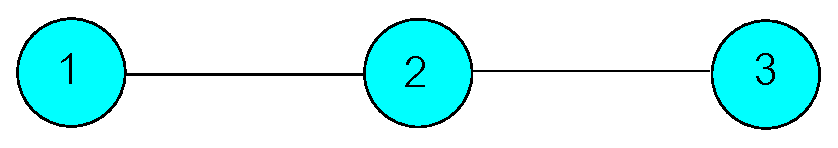
\includegraphics[width=3in]{figure/3nodes-chain}
\caption{A simple multi-hop network.}
\label{fig:3nodes-chain}
\end{figure}

\begin{figure}[!t]
\centering
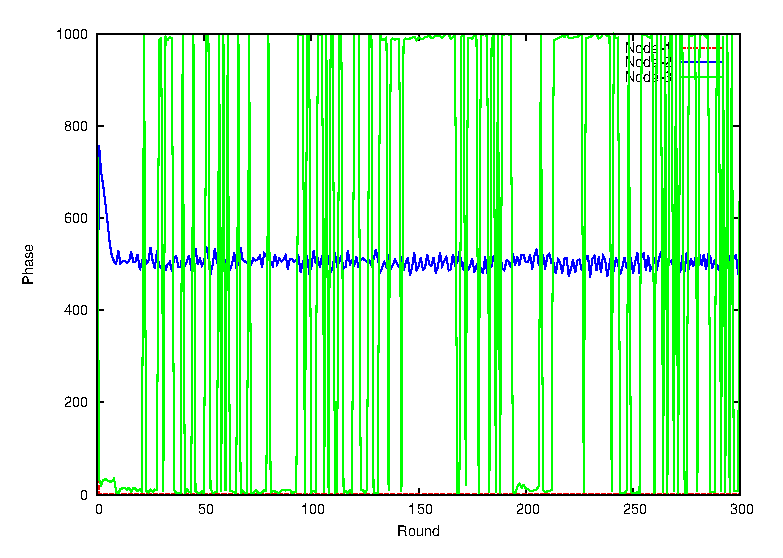
\includegraphics[width=3.5in]{figure/3nodes-chain-dwarf}
\caption{Message collision on a 3-node multi-hop chain network. The period T is 1000 milliseconds. Node 1 is at phase 0 whereas node 3 is approximately at the same phase as node 1.}
\label{fig:3nodes-chain-dwarf}
\end{figure}

\begin{figure}[!t]
\centering
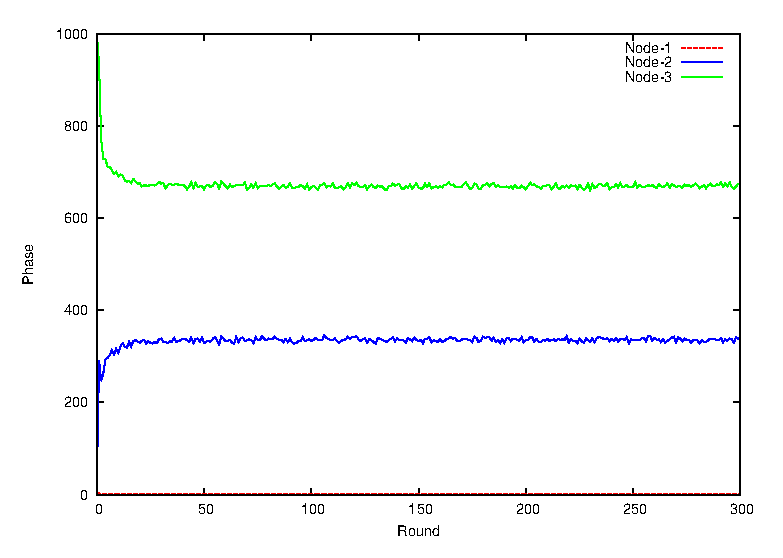
\includegraphics[width=3.5in]{figure/3nodes-chain-expected}
\caption{The perfect desynchrony state of a 3-node multi-hop chain network, The period T is 1000 milliseconds. Node 1 is at phase 0 whereas others are separated by T/3 milliseconds.}
\label{fig:3nodes-chain-expected}
\end{figure}

We have simulated DWARF by setting the period to 1000 milliseconds. Nodes wake up randomly. 
The simulation result is shown in Figure \ref{fig:3nodes-chain-dwarf}. Node 2's and node 3's phases are plotted relatively to the node 1's phase (\textit{i.e.}, the node 1's phase is relatively plotted to itself at 0). The noisy vertical line is the wrapping-around phase of node 3. The result shows that node 1 and node 3 fire messages approximately at the same phase. This causes the message collision at node 2.
However, the expected result (\textit{i.e.} perfect desynchrony state) should be that three nodes are separated equivalently because all nodes will interfere each other if they fire messages at the same phase. The expected result is shown in Figure \ref{fig:3nodes-chain-expected} where each node is equivalently separated from each other approximately by 1000/3 milliseconds.

The problematic result is caused by the hidden terminal problem as demonstrated in Figure \ref{fig:3nodes-chain-hidden}; node 1 and node 3 are hidden to each other in this multi-hop topology. While node 3 is firing a message, node 1 senses a wireless channel and does not detect any signal from node 3 because the signal from node 3 is not strong enough within the signal sensing range of node 1 and vice versa. Therefore, in DWARF, node 1 and node 3 notice only that there are two nodes, which are itself and node 2, in their perceived networks. Therefore, node 1 and node 3 simultaneously attempt to adjust their phases to the opposite side of node 2 in their time circles which are the same phase. As a result, their firing messages collide at node 2. 

\begin{figure}[!t]
\centering
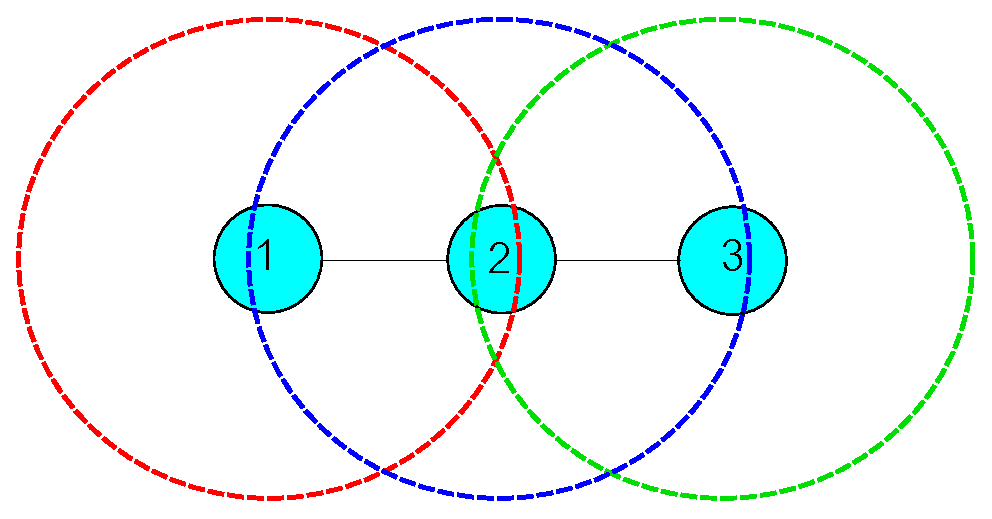
\includegraphics[width=4in]{figure/3nodes-chain-hidden}
\caption{The hidden terminal problem.}
\label{fig:3nodes-chain-hidden}
\end{figure}

The hidden terminal problem does not only affect the performance of DWARF but also affect that of DESYNC.
This is due to the fact that, in DESYNC, a node adjusts its phase based on firing messages from its perceived phase neighbors. In \cite{4663417} and \cite{MK09DESYNC}, EXTENDED-DESYNC, which is the extension of DESYNC, is proposed to solve the hidden terminal problem based on a relative time relaying mechanism. Based on the similar idea, we extend DWARF to support multi-hop topologies.
However, only relative time relaying mechanism does not lead DWARF to an optimal solution in some cases. Therefore, this dissertation also proposes a \textit{force absorption} mechanism for extending DWARF to support multi-hop networks.   

\section{DWARF with Multi-hop Extension (M-DWARF)}
\label{sec:extension}
\subsection{Relative Time Relaying}
\label{sec:relative}
The first idea to solve the hidden terminal problem is straightforward. If a node does not know the firing times of its second-hop neighbors, its one-hop neighbors relay such information. Therefore, instead of firing only to notify its firing time, each node includes their one-hop neighbors' firing times into a firing message. 

However, due to our assumption that nodes' clocks are not synchronized, relying on second-hop neighbors' firing timestamps from its one-hop neighbors could lead to wrong phase adjustment. This problematic scenario is demonstrated in Figure \ref{fig:broadcast-problem}. Figure \ref{fig:broadcast-problem-topo} illustrates the firing message of node 2 that contains timestamps of its one-hop neighbors. Figure \ref{fig:broadcast-problem-ring} shows the problem. The inner circle represents the local time of node 1 and the outer circle represents the local time of node 2. The figure indicates that the local reference times (at 0 millisecond) of node 1 and node 2 are different. Therefore, if node 1 uses the node 3's firing time relayed by node 2, which is 125 milliseconds, node 1 will misunderstand the exact time phase of node 3. The misunderstood phase of node 3 is depicted as a dash circle. 

\begin{figure*}[!t]
\centerline{
	\subfloat[]{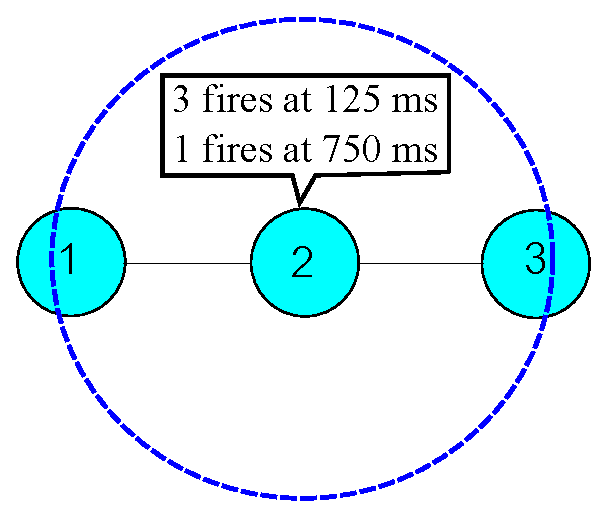
\includegraphics[scale=0.60]{figure/broadcast-problem-topo}%
	\label{fig:broadcast-problem-topo}}
	\hfil
	\subfloat[]{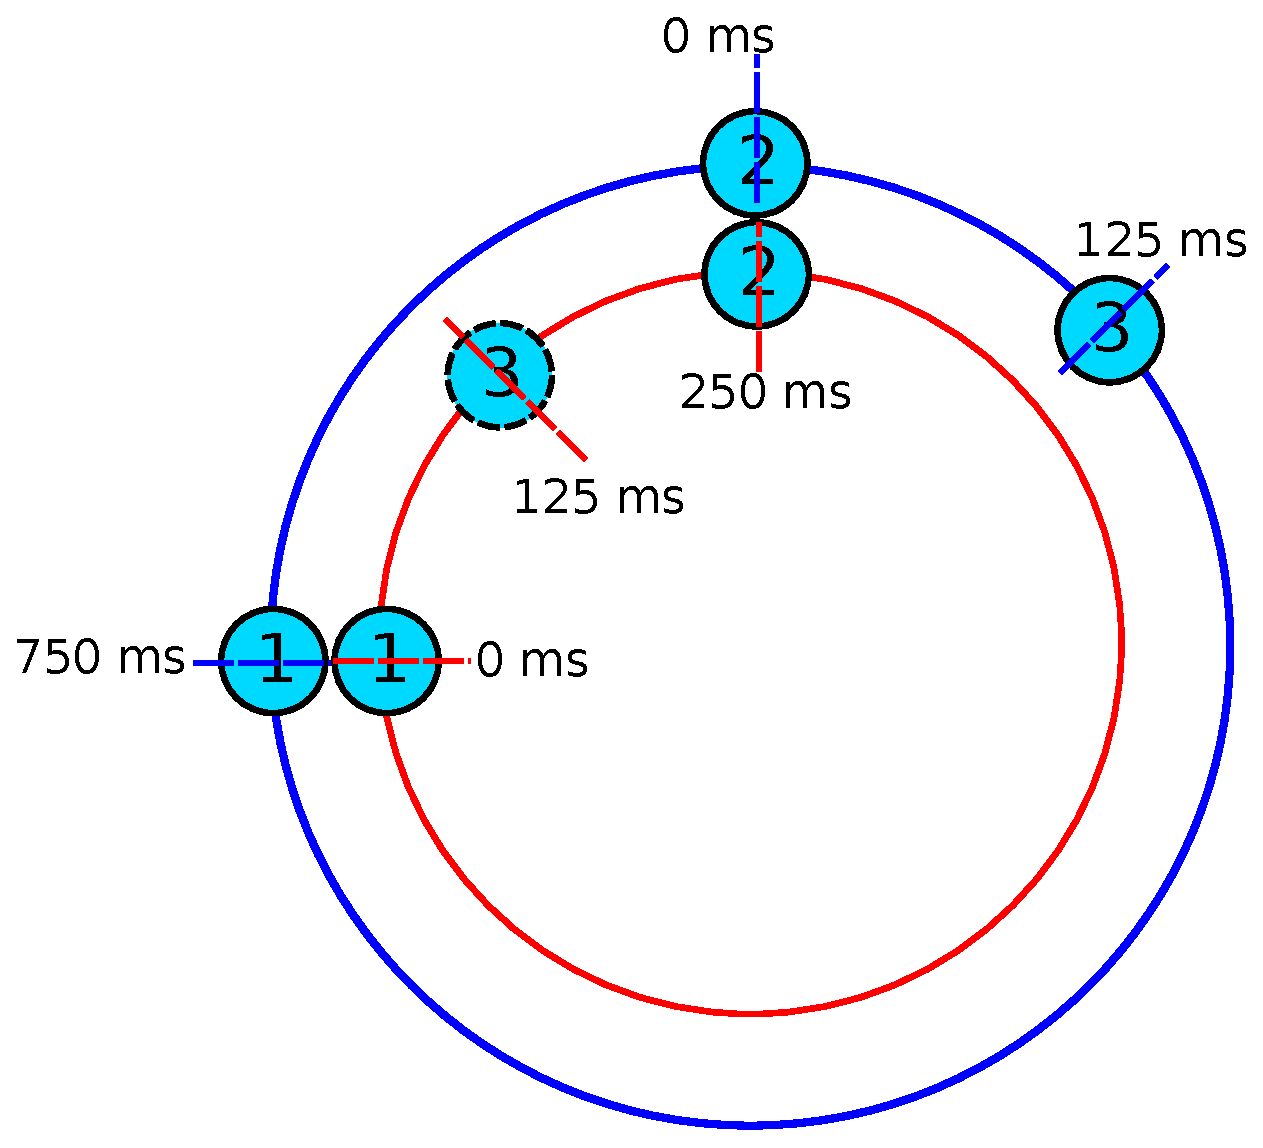
\includegraphics[scale=0.35]{figure/broadcast-problem-ring}%
	\label{fig:broadcast-problem-ring}}
}
\caption{A node includes its one-hop neighbors' firing times into a firing message. (a) Node 2 fires a message containing node 1's and node 2's firing timestamps that it perceives. (b) Node 1 misunderstands the time phase of node 3 because local time of node 1 and local time of node 2 are different.}
\label{fig:broadcast-problem}
\lofcont
\end{figure*}

This problem can be simply solved by using relative phases instead of actual local times. Each node fires a message that includes relative phases of its one-hop neighbors. A receiving node marks the firing phase of the firing node as a reference phase. Then, the receiving node perceives its second-hop neighbors' phases as relative phases offset by the reference phase. Figure \ref{fig:broadcast-relative} shows how extended DWARF desynchronizes a 3-node multi-hop chain network.

\begin{figure*}[!t]
\centerline{
	\subfloat[]{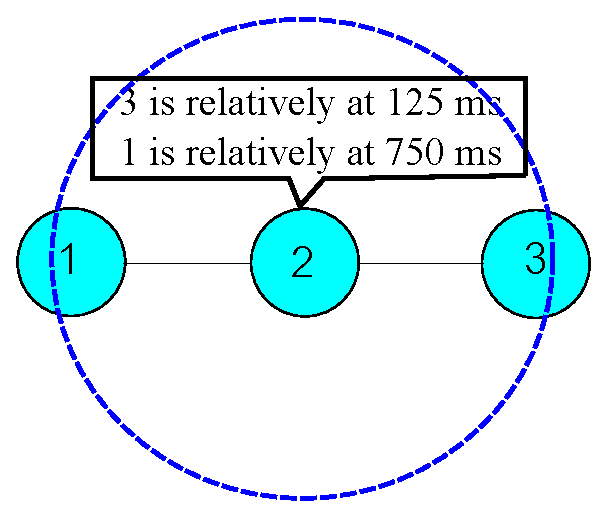
\includegraphics[scale=0.45]{figure/broadcast-relative-topo}%
	\label{fig:broadcast-relative-topo}}
	\hfil
	\subfloat[]{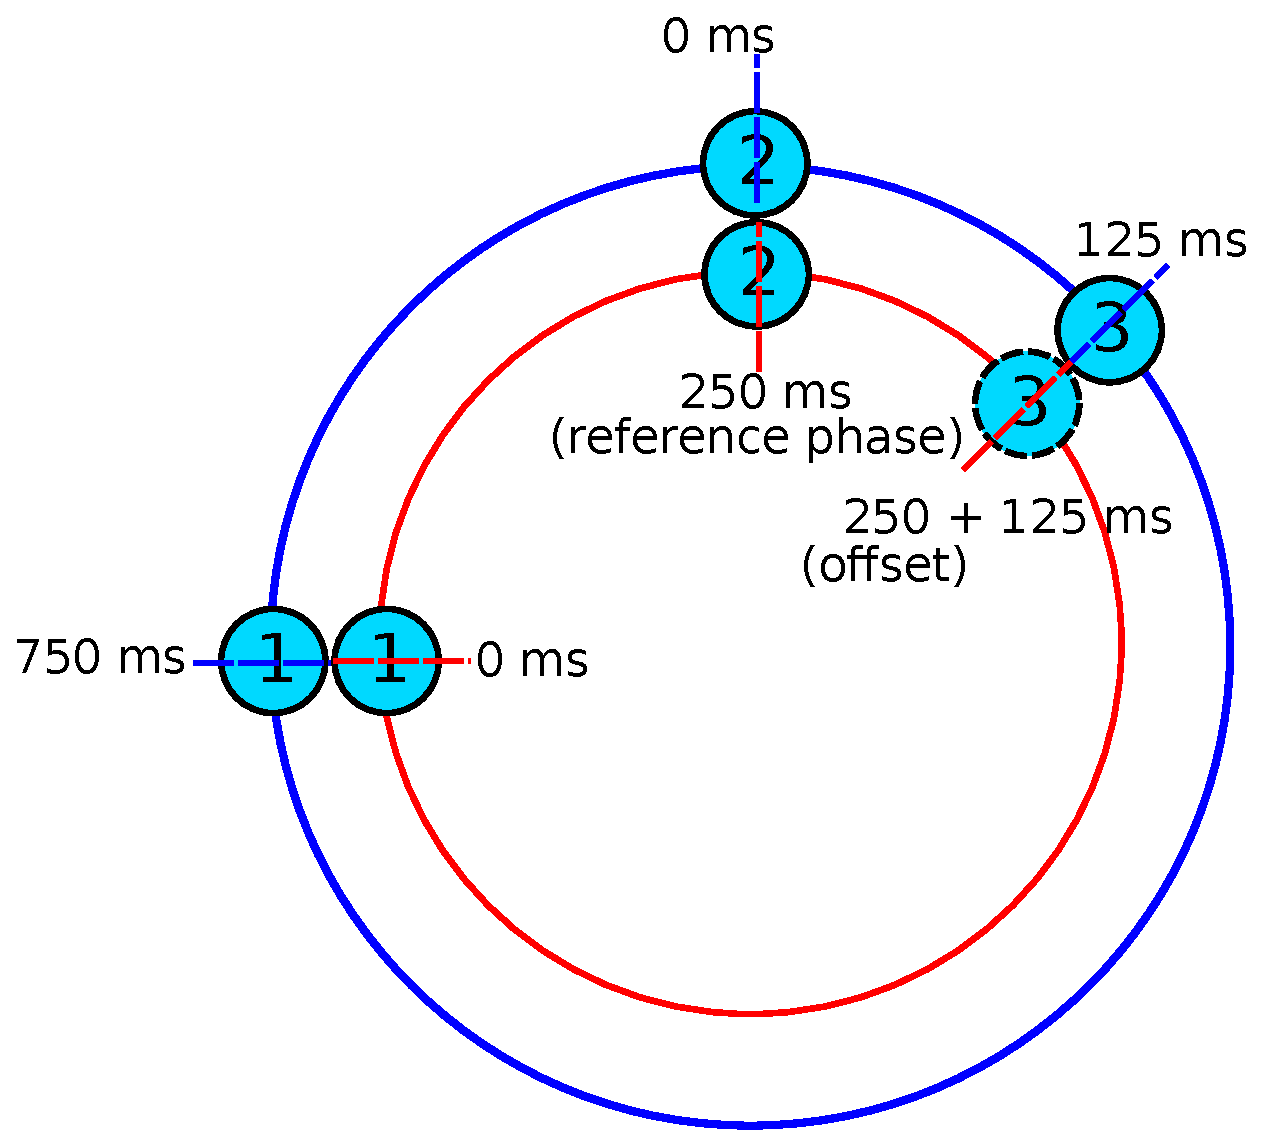
\includegraphics[scale=0.25]{figure/broadcast-relative-ring}%
	\label{fig:broadcast-relative-ring}}
	\hfil
	\subfloat[]{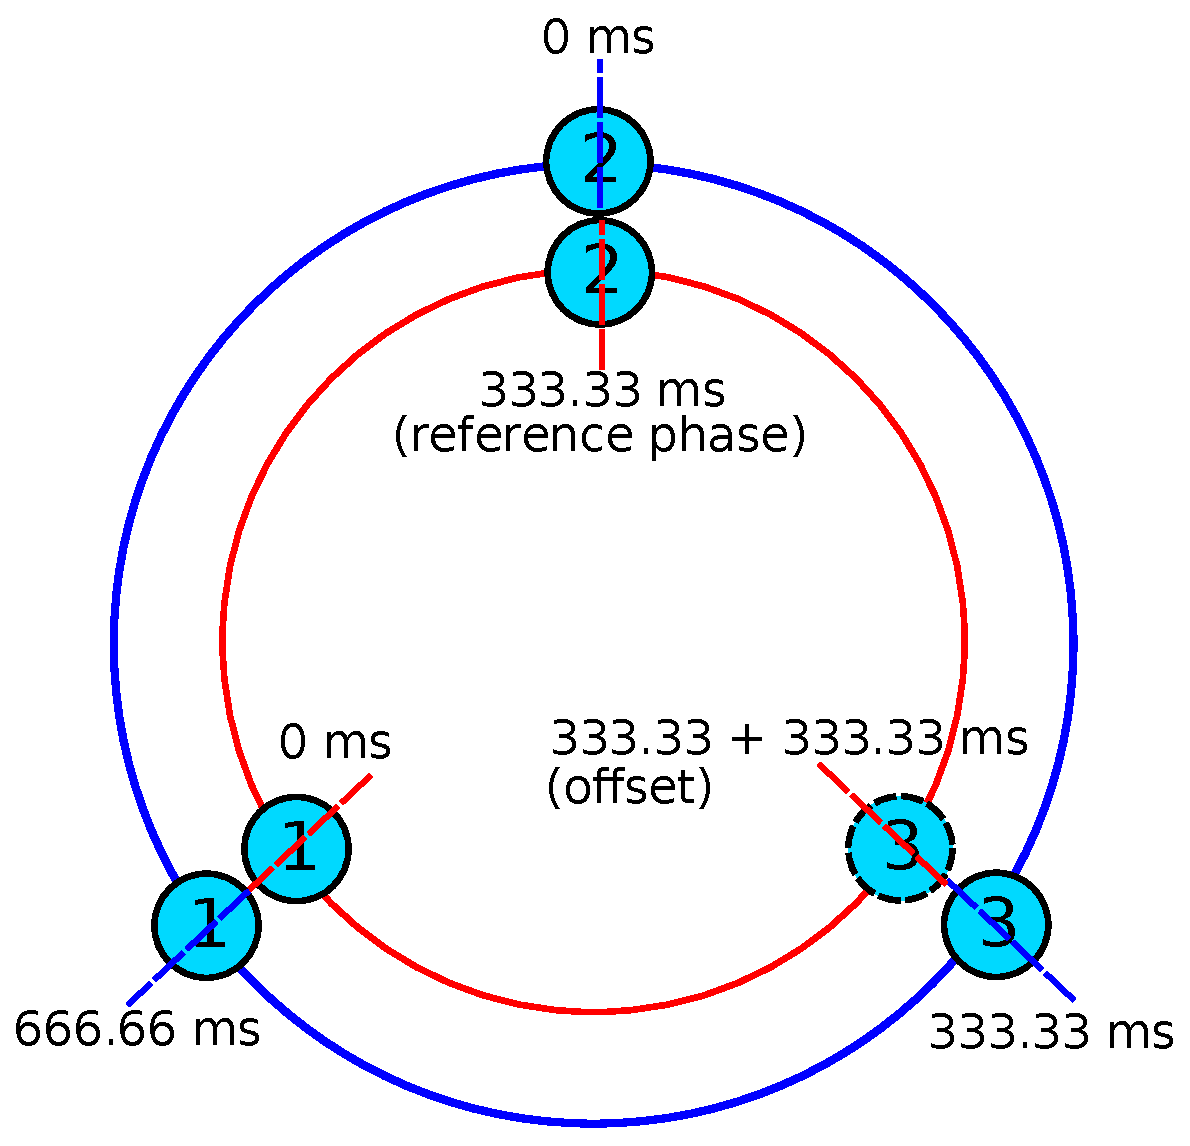
\includegraphics[scale=0.25]{figure/broadcast-relative-perfect}%
	\label{fig:broadcast-relative-perfect}}
}
\caption{EXT-DWARF: A node includes its one-hop neighbors' relative phases into a firing message. (a) Node 2 fires a message containing node 1's and node 2's relative phases. (b) Node 1 marks the node 2's phase as a reference phase and uses it as an offset for calculating the node 3's phase. (c) Eventually, nodes are in the perfect desynchrony state.}
\label{fig:broadcast-relative}
\lofcont
\end{figure*}


\subsection{Force Absorption}
\label{sec:absorption}
As we mentioned earlier, DWARF with the relative time relaying mechanism does not solve some cases.
These cases are when there are at least two second-hop neighbors that can share the same phase without interference. For example, in a 4-node chain network illustrated in Figure \ref{fig:4nodes-chain-topo}, node 2 and node 3 are physically far beyond two hops. Therefore, they can fire messages at the same time phase as shown in Figure \ref{fig:4nodes-chain-expected}.
However, in extended DWARF, node 0 perceives that node 2 and node 3 are at the same phase. Therefore, there are two forces from node 2 and node 3 to repel node 0 forward but there is only force from node 1 to repel node 0 backward. Consequently, node 0 cannot stay at the middle between node 1 and the group of node 2 and 3 (see Figure \ref{fig:4nodes-chain-dwarf}). 

\begin{figure*}[!t]
\centerline{
	\subfloat[]{\includegraphics[scale=0.3]{figure/4nodes-chain-topo}%
	\label{fig:4nodes-chain-topo}}
	\hfill
	\subfloat[]{\includegraphics[scale=0.20]{figure/4nodes-chain-expected}%
	\label{fig:4nodes-chain-expected}}
	\hfill
	\subfloat[]{\includegraphics[scale=0.20]{figure/4nodes-chain-dwarf}%
	\label{fig:4nodes-chain-dwarf}}
}
\caption{The problem of the single-hop DWARF algorithm. (a) A 4-node chain topology. The transmission signal of node 2 does not interfere any receiver of node 3 and vice versa. (b) In the node 0's local view, the expected result is that node 2 and node 3 can share the same phase without interference. (c) In extended DWARF, node 0 is not in the expected phase because there are two forward repelling forces from node 2 and node 3 while there is one backward repelling force from node 1.}
\label{fig:4nodes-chain}
\lofcont
\end{figure*}

Therefore, we propose a novel force absorption mechanism for multi-hop desynchronization based on the artificial force field.
The objective of this mechanism is to absorb the overwhelming force from at least two nodes that can fire at the same phase without interference.

The mechanism is as follows. A node receives a full repelling force from the next/previous phase neighbor as in DWARF. However, a force from the second-next/second-previous phase neighbor is partially absorbed by the next/previous phase neighbor. The magnitude of the absorbed force depends on the phase interval between the next/previous and the second-next/second-previous phase neighbors.  The closer that the second-next/second-previous phase neighbor moves to the next/previous phase neighbor results in the lower magnitude of the absorbed force. Eventually, when the second-next/second-previous phase neighbor moves to the same phase as the next/previous phase neighbor, the additional force from the second-next/second-previous phase neighbor is fully absorbed. Consequently, the magnitude of two forces repelling the considered node is approximately equal to only magnitude of one force. This principle is applied recursively; the force from the third-next/third-previous phase neighbor is absorbed by the second-next/second-previous phase neighbor, the force from the fourth-next/fourth-previous phase neighbor is absorbed by the third-next/third-previous phase neighbor, and so forth.   
Figure \ref{fig:4nodes-chain-dwarf-absorb} illustrates this mechanism. In Figure \ref{fig:4nodes-chain-dwarf-absorb-split}, the force from node 2 to node 0 is absorbed by node 3 (the absorbed force is displayed in a blur line). Thus, from node 2, there is only small magnitude of force left to node 0. Eventually, in Figure \ref{fig:4nodes-chain-dwarf-absorb-perfect}, node 2 moves to the same phase as node 3 because they do not interfere each other and the force from node 2 is fully absorbed. Consequently, the network can be in the perfect desynchrony state.

\begin{figure*}[!t]
\centerline{
	\subfloat[]{\includegraphics[scale=0.33]{figure/4nodes-chain-dwarf-absorb-split}%
	\label{fig:4nodes-chain-dwarf-absorb-split}}
	\hfil
	\subfloat[]{\includegraphics[scale=0.33]{figure/4nodes-chain-dwarf-absorb-perfect}%
	\label{fig:4nodes-chain-dwarf-absorb-perfect}}
}
\caption{EXT-DWARF with force absorption. The blur line represented an absorbed force. (a) When node 2 and 3 are apart, the force from node 2 affects node 0 but the force is partly absorbed. (b) When node 2 and 3 are at the same phase, the force from node 2 is fully absorbed.}
\label{fig:4nodes-chain-dwarf-absorb}
\lofcont
\end{figure*}

Let $f_{i,j}$ be a full repelling force from node $j$ to node $i$, $f_{i,j}^{'}$ be an absorbed force from node $j$ to node $i$, $T$ is the time period, and $\Delta \phi_{i,j}$ is the phase difference between node $i$ and $j$. 
The force function for multi-hop networks is the following:
\begin{alignat}{2}
f_{i,j} &= \frac{1}{\Delta \phi_{i,j} / T}, \text{where }\Delta \phi_{i,j} \in (-\frac{T}{2}, \frac{T}{2}) \nonumber \\
f_{i,i + 1}^{'} &= f_{i,i + 1} \nonumber \\
f_{i, i - 1}^{'} &= f_{i,i - 1} \nonumber \\
f_{i,j}^{'} &= f_{i,x} - f_{i,j}, \text{where } j \notin \left\{i -1, i + 1\right\} \text{ and } x = (j - \frac{\Delta \phi_{i,j}}{|\Delta \phi_{i,j}|}) \mod n.
\label{eq:force-absorb}
\end{alignat}
For $f_{i,x}$, if node $j$ repels node $i$ forward, $x$ is $j + 1$. In contrast, if node $j$ repels node $i$ backward, $x$ is $j - 1$. At $T/2$ or $-T/2$, a node does not repel an opposite node because they are balanced.

For example, in Figure \ref{fig:4nodes-chain-dwarf-absorb}, node 0 calculates the force from node 2 as the following:
\begin{alignat}{2}
f_{0,2}^{'} &= f_{0,3} - f_{0,2} \nonumber \\
&= \frac{1}{\Delta \phi_{0,3} / T} - \frac{1}{\Delta \phi_{0,2} / T}. \nonumber
\end{alignat} 

Noticeably, if node 2 moves close to node 3, the value of $\Delta \phi_{0,2}$ is close to the value of $\Delta \phi_{0,3}$. Then, the magnitude of force $f_{0,2}$ is reduced. 
Finally, when $\Delta \phi_{0,2}$ is equal to $\Delta \phi_{0,3}$ as in Figure \ref{fig:4nodes-chain-dwarf-absorb-perfect}, the magnitude of force $f_{0,2}$ becomes 0. In other words, the force is fully absorbed. 

\section{M-DWARF Algorithm}
\label{sec:multihop-algo}
The M-DWARF algorithm is similar to DWARF (see Chapter \ref{chap:algo}). However, M-DWARF has two proposed mechanisms to support multi-hop topologies: relative time relaying and force absorption. Initially, nodes are not desynchronized. 
Each node sets a timer to fire in $T$ time unit and listens to all one-hop neighbors.

When receiving a firing message from its one-hop neighbor, the receiving node marks the current time to be the relative phase reference. Then, the node reads relative phases of its two-hop neighbors which are included within the firing message. After that, the node calculates their two-hop neighbors' phases by using the relative phase reference as the offset.  

When the timer expires, the node broadcasts a firing message containing relative phases of its one-hop neighbors. 
Then, the node calculates a new time phase to move on the phase circle. The calculation is based on the summation of artificial forces from all phase neighbors within two-hops where some forces are absorbed. Then, the node sets a new timer according to the new calculated phase.

As same as DWARF, a node adjusts its phase as follows.
Given the total received absorbed force $\mathcal{F}_i$, the node $i$ adjusts to a new time phase $\phi_i^{'}$,
\begin{equation}
\phi_i^{'} = (\phi_i + K\mathcal{F}_i) \mod T,
\label{eq:newphase-mhop}
\end{equation} 
where $\phi_i$ is the current phase of the node $i$.

We choose the coefficient $K$ as same as in DWARF: 
\begin{equation}
K = 38.597 \times n^{-1.874} \times \frac{T}{1000},
\end{equation}
where $n$ is the number of phase neighbors within two hops and $T$ is the time period.
We refer to Section \ref{sec:algo} that proves and describes in details how we get the value of the coefficient $K$. In short, the value of the coefficient $K$ is inverse proportional to the number of nodes $n$ and proportional to the time period $T$.

All nodes in the artificial force field (in the period circle) iteratively run the same algorithm until the force is balanced.
The pseudo-code of this algorithm is shown in Figure \ref{fig:pseudocodemdwarf}.


\begin{figure}[!t]
\begin{algorithmic}[1]
	\STATE \textbf{Initialization}  
  	\STATE $T = TimePeriod$ \COMMENT{Configurable Time Period}
  	\STATE $n = 1$ \COMMENT{Number of neighbors within two hops including itself}
  	\STATE $\mathcal{F} = 0$ \COMMENT{Force Summation}
  	\STATE $phasesBuffer = Array$ \COMMENT{Buffer for phases of neighbors within two hops}
  	\STATE $lastFiringTime = localTime$
  	\STATE $currentPhase = localTime$ modulo $T$
  	\STATE Set a firing timer to be $T$ unit time
  	\newline
  	
  	\STATE \textbf{Upon timer firing}
    \STATE Broadcast a firing message containing relative phases of one-hop neighbors
    \STATE $lastFiringTime = localTime$
  	\STATE $currentPhase= localTime$ modulo $T$
    \STATE $K = 38.597 \times n^{-1.874} \times \frac{T}{1000}$
    \STATE $\mathcal{F}$ = call Calculate total force
    \STATE $newPhase = currentPhase + (K \times \mathcal{F})$
    \IF{$newPhase < 0$}
    	\STATE $newPhase = T + newPhase$
	\ENDIF
    \STATE Set a firing timer to be fired at ($newPhase$ modulo $T$)
   	\STATE $\mathcal{F} = 0$
   	\STATE $n = 1$
 	\newline
 	
 	\STATE \textbf{Calculate total force}
 	\STATE $sortedBuffer$ = Sort $phasesBuffer$
 	\STATE $forwardForce = \frac{1}{(T - sortedBuffer[length - 1])/T}$
 	\STATE $backwardForce = \frac{1}{sortedBuffer[0]/T}$
    \FOR{$i$ in range of 1 to length of sorted $phasesBuffer$ - 2}
      \IF{$phasesBuffer[i] > 0.5T$}
        \STATE $forwardForce = forwardForce + (\frac{1}{(T - phasesBuffer[i+1]) / T} - \frac{1}{(T - phasesBuffer[i]) / T})$
      \ELSE
        \STATE $backwardForce = backwardForce + (\frac{1}{phaseBuffer[i-1] / T} - \frac{1}{phaseBuffer[i] / T})$
      \ENDIF
    \ENDFOR
    \STATE return $forwardForce - backwardForce$
 	\newline
 	   
    \STATE \textbf{Upon receiving a firing message from $nodeId$}
    \STATE $phaseDiff = localTime - lastFiringTime$
    \STATE $phasesBuffer[nodeId] = phaseDiff$
    \STATE $reference = phaseDiff$
    \FOR{each $twoHopNodeId$ of two-hop neighbors in $message$}
      \IF{$twoHopNodeId$ is not in $phasesBuffer$} 
        \STATE $phasesBuffer[twoHopNodeId] = message[twoHopNodeId][relativePhase] + reference$
        \STATE $n = n + 1$
      \ENDIF
    \ENDFOR
\end{algorithmic}
\caption{Pseudocode of M-DWARF algorithm}
\label{fig:pseudocodemdwarf}
\end{figure}

\section{Evaluation}
\label{sec:multihop-evaluation}
In this section, we evaluate the performance of M-DWARF, EXTENDED-DESYNC (\cite{MK09DESYNC}), and LIGHTWEIGHT (\cite{5062165}). All of these algorithms do not require time synchronization. We begin by measuring the desynchronization error and convergence time on single-hop networks because the extension for multi-hop networks should work on single-hop networks as well. Then, we evaluate on several multi-hop topologies which are used in the previous work (\cite{4663417}).

\subsection{Evaluation Environment}
We implement M-DWARF, EXTENDED-DESYNC, and LIGHTWEIGHT on Tiny-OS 2.1.2 and evaluate them on the TOSSIM simulator.
In our simulation, for all algorithms, we use 2-byte sender node ID, and 2-byte neighbor ID. For M-DWARF and EXTENDED-DESYNC, we use 2-byte relative phase for each one-hop neighbor. The regular 11-byte CC2420 header is also used.
The time period is set to 1000, 2000, and 3000 milliseconds.
The step size ($\alpha$) of EXTENDED-DESYNC is set to 0.95 as same as in Chapter \ref{chap:algo}.
The phase of each node is initially random in a range of 0 to the period length 


\subsection{Single-hop Networks (Fully-connected Topology) Evaluation}
We begin by evaluating M-DWARF on single-hop networks. In M-DWARF and EXTENDED-DESYNC, each firing message contains relative phases of one-hop neighbors. Therefore, to limit the size of a message, we vary the one-hop network size from 4 to 32 nodes.

\subsubsection{Desynchronization Error}
We run the simulation for 300 time periods to measure the desynchronization error. 
In each network size, we run the simulation for 30 times.
Then, we measure the average root mean square error (RMSE) and normalized root mean square error (see details in Section \ref{sec:error}). 
Figure  \ref{fig:rmse300rounds-mhop} illustrates the result of absolute desynchronization error and Figure \ref{fig:nrmse300rounds-mhop} illustrates the result of the normalized desynchronization error in each network size after 300 time periods.

\begin{figure*}[!t]
\centerline {
	\subfloat[]{\includegraphics[width=3.0in]{figure/compare300rounds_rmse_sd_mhop}%
	\label{fig:rmse300rounds-mhop}}
	\hfil
	\subfloat[]{\includegraphics[width=3.0in]{figure/compare300rounds_nrmse-expected_sd_mhop}%
	\label{fig:nrmse300rounds-mhop}}
}
\caption{(a) Root mean square error after 300 time periods. (b) Root mean square error normalized by perfect phase difference after 300 time periods.}
\lofcont
\end{figure*}

The result indicates that, in all network sizes (4 - 32 nodes), M-DWARF achieves significantly better desynchrony states than EXTENDED-DESYNC and LIGHTWEIGHT do. 
The EXTENDED-DESYNC's mechanism has the same pitfall as that of DESYNC because they are based on the same mechanism. The pitfall is that the phase error of a node propagates to its phase neighbors and this error will propagate back and forth between two phase neighbors. This results in a large error after convergence.
In contrast, M-DWARF is robust to this error propagation as same as DWARF because both M-DWARF and DWARF use the total received forces from all neighbors. An error from one neighbor does not overwhelm the system.
For LIGHTWEIGHT, the desynchronization errors of small networks are extremely large because the algorithm randomly chooses the free time slot without considering the equitably separation. However, when the network size becomes larger, the error becomes lower because the perfect phase interval length is reduced.

\begin{figure*}[!t]
\centerline{
	\subfloat[Sparse]{\includegraphics[width=3.0in]{figure/compare-rmse-4-8nodes_sd_mhop}%
	\label{fig:rmse-sparse-mhop}}
	\hfil
	\subfloat[Dense]{\includegraphics[width=3.0in]{figure/compare-rmse-16-32nodes_sd_mhop}%
	\label{fig:rmse-dense-mhop}}
}
\caption{Convergence time and absolute root mean square error}
\label{fig:rmse-convergence-mhop}
\lofcont
\end{figure*}

\begin{figure*}[!t]
\centerline{
	\subfloat[Sparse]{\includegraphics[width=3.0in]{figure/compare-nrmse-4-8nodes_sd_mhop}%
	\label{fig:nrmse-sparse-mhop}}
	\hfil
	\subfloat[Dense]{\includegraphics[width=3.0in]{figure/compare-nrmse-16-32nodes_sd_mhop}%
	\label{fig:nrmse-dense-mhop}}
}
\caption{Convergence time and root mean square error normalized by expected phase difference}
\label{fig:nrmse-convergence-mhop}
\lofcont
\end{figure*}

\subsubsection{Convergence Time}
\begin{figure*}
\centerline{
  \subfloat[8 nodes]{\includegraphics[scale=0.5]{figure/fluctuate-8}}
  \hfil
  \subfloat[16 nodes]{\includegraphics[scale=0.5]{figure/fluctuate-16}}
}
\caption{Fluctuation in some cases of EXTENDED-DESYNC.}
\label{fig:fluctuate}
\lofcont
\end{figure*}
In this section, we measure the absolute root mean square error and normalized root mean square error for each time period to investigate the convergence time.
Figure \ref{fig:rmse-sparse-mhop} and \ref{fig:nrmse-sparse-mhop} show the results of sparse networks whereas Figure \ref{fig:rmse-dense-mhop} and \ref{fig:nrmse-dense-mhop} show the results of dense networks.

In all network sizes, the convergence speed of M-DWARF is comparable to that of EXTENDED-DESYNC. However, M-DWARF converges with the lowest desynchronization error. For LIGHTWEIGHT, the algorithm converges fast and stable. However, due to the random slot selection process, the desynchronization errors in all network sizes are large.

We note that the errors of EXTENDED-DESYNC for 8-node and 16-node networks are fluctuate. This is due to the fact that, in our 30 EXTENDED-DESYNC simulations, there are some cases in 8-node and 16-node networks that the phases of some nodes are highly fluctuate as depicted in Figure \ref{fig:fluctuate}. These cases affect the average value. This behaviour is caused by the mechanism of EXTENDED-DESYNC (and DESYNC) that relies on only two phase neighbors information as described earlier in Chapter \ref{chap:algo}.

The result of single-hop networks indicates that M-DWARF that augments DWARF with two mechanisms still performs very well on single-hop networks without loss of generality. 


\subsection{Impact of Topologies}
For multi-hop networks, we evaluate M-DWARF on several topologies including star, chain, cycle, butterfly, and mesh topologies. In each topology, we simulate for 30 times and show the relative phase graph results. We show the phase graphs that represent the average case and the problematic case of each algorithm. We note that, in all topologies, LIGHTWEIGHT achieves the similar results. For LIGHTWEIGHT, each node randomly chooses the beginning of a time slot by avoiding the collision with one-hop neighbors. Therefore, on average, LIGHTWEIGHT causes several inequivalent interval gaps between two consecutive phase neighbor nodes. Moreover, there are several problematic cases that at least two nodes within two-hop communication choose the same beginning of a time slot because they cannot receive firing messages from each other. Thus, in all topologies, we only describe the behaviour of M-DWARF and EXTENDED-DESYNC.

\begin{figure*}[!t]
\centering{
	\subfloat[6 nodes]{\includegraphics[scale=0.4]{figure/6nodes-star-eval}%
	\label{fig:6nodes-star-eval}}
	\hspace{1in}
	\subfloat[20 nodes]{\includegraphics[scale=0.25]{figure/20nodes-star-eval}%
	\label{fig:20nodes-star-eval}}
}
\caption{Star topology}
\label{fig:star-eval}
\lofcont
\end{figure*}

\subsubsection{Star Topology}
\begin{figure*}[!t]
\centering{
	\subfloat[M-DWARF]{\includegraphics[scale=0.35]{figure/6nodes-star-result-mdwarf-good}%
	\label{fig:6nodes-star-result-mdwarf-good}}
	\hfil
	\subfloat[EXTENDED-DESYNC]{\includegraphics[scale=0.35]{figure/6nodes-star-result-extdesync-good}%
	\label{fig:6nodes-star-result-extdesync-good}}
	\hfil
	\subfloat[LIGHTWEIGHT]{\includegraphics[scale=0.35]{figure/6nodes-star-result-light-good}%
	\label{fig:6nodes-star-result-light-good}}
}
\caption{6-node star topology evaluation (average case).}
\label{fig:6nodes-star-result-good}
\lofcont
\end{figure*}
\begin{figure*}[!t]
\centering{
	\subfloat[M-DWARF]{\includegraphics[scale=0.35]{figure/20nodes-star-result-mdwarf-good}%
	\label{fig:20nodes-star-result-mdwarf-good}}
	\hfil
	\subfloat[EXTENDED-DESYNC]{\includegraphics[scale=0.35]{figure/20nodes-star-result-extdesync-good}%
	\label{fig:20nodes-star-result-extdesync-good}}
	\hfil
	\subfloat[LIGHTWEIGHT]{\includegraphics[scale=0.35]{figure/20nodes-star-result-light-good}%
	\label{fig:20nodes-star-result-light-good}}
}
\caption{20-node star topology evaluation (average case).}
\label{fig:20nodes-star-result-good}
\lofcont
\end{figure*}
The star topology is the simplest case for multi-hop desynchronization. There is one center node that can transmit and receive messages with all other nodes in the network. In contrast, other nodes can  transmit and receive only with the center node. Figure \ref{fig:star-eval} illustrates 6-node and 20-node star topologies that we use for algorithms evaluation. In the star topology, every node is connected to each other within two-hop communication. As a result, all nodes must use different time slots. 

Figure \ref{fig:6nodes-star-result-good} and \ref{fig:20nodes-star-result-good} shows the simulation results of three algorithms on 6-node and 20-node star topologies respectively.
Due to the relative phase relaying mechanism, both M-DWARF and EXTENDED-DESYNC perceive relative phases of neighbors within two hops, which are all nodes in the system. Consequently, both algorithms can separate 6 nodes into almost equivalent 6 time slots. However, M-DWARF achieves almost perfect desynchony whereas EXTENDED-DESYNC slightly fluctuates in the sparse 6-node network and highly fluctuates in the dense 20-node network.
\begin{figure*}[!t]
\centering{
	\subfloat[M-DWARF]{\includegraphics[scale=0.35]{figure/6nodes-star-result-mdwarf-bad}%
	\label{fig:6nodes-star-result-mdwarf-bad}}
	\hfil
	\subfloat[EXTENDED-DESYNC]{\includegraphics[scale=0.35]{figure/6nodes-star-result-extdesync-bad}%
	\label{fig:6nodes-star-result-extdesync-bad}}
	\hfil
	\subfloat[LIGHTWEIGHT]{\includegraphics[scale=0.35]{figure/6nodes-star-result-light-bad}%
	\label{fig:6nodes-star-result-light-bad}}
}
\caption{6-node star topology evaluation (problematic case).}
\label{fig:6nodes-star-result-bad}
\lofcont
\end{figure*}
\begin{figure*}[!t]
\centering{
	\subfloat[M-DWARF]{\includegraphics[scale=0.35]{figure/20nodes-star-result-mdwarf-bad}%
	\label{fig:20nodes-star-result-mdwarf-bad}}
	\hfil
	\subfloat[EXTENDED-DESYNC]{\includegraphics[scale=0.35]{figure/20nodes-star-result-extdesync-bad}%
	\label{fig:20nodes-star-result-extdesync-bad}}
	\hfil
	\subfloat[LIGHTWEIGHT]{\includegraphics[scale=0.35]{figure/20nodes-star-result-light-bad}%
	\label{fig:20nodes-star-result-light-bad}}
}
\caption{20-node star topology evaluation (problematic case).}
\label{fig:20nodes-star-result-bad}
\lofcont
\end{figure*}
Figure \ref{fig:6nodes-star-result-bad} and \ref{fig:20nodes-star-result-bad} shows the problematic cases. For M-DWARF, there is no problem in the sparse networks, but, in the dense networks, nodes take more time to become stable. The reason is that, when the network is dense, the usable time interval gap for each node is shortened. Therefore, if several nodes start closely to each other at the initial configuration, forces are highly absorbed. As a result, they takes more time to separate away from each other. In the case of EXTENDED-DESYNC, the fluctuated error from one node can propagate throughout the networks because each node relies on only information of two phase neighbors.




\subsubsection{Chain Topology}
The chain topology is one of the simplest topologies. Every node is lined up without a loop. The 3-node and 10-node chain topologies are depicted in Figure \ref{fig:chain-eval}. 
\begin{figure*}[!t]
\centering{
	\subfloat[3 nodes]{\includegraphics[scale=0.45]{figure/3nodes-chain-eval}%
	\label{fig:3nodes-chain-eval}}
	\hspace{1in}
	\subfloat[10 nodes]{\includegraphics[scale=0.35]{figure/10nodes-chain-eval}%
	\label{fig:10nodes-chain-eval}}
}
\caption{Chain topology}
\label{fig:chain-eval}
\lofcont
\end{figure*}
\begin{figure*}[!t]
\centering{
	\subfloat[M-DWARF]{\includegraphics[scale=0.35]{figure/3nodes-chain-result-mdwarf-good}%
	\label{fig:3nodes-chain-result-mdwarf-good}}
	\hfil
	\subfloat[EXTENDED-DESYNC]{\includegraphics[scale=0.35]{figure/3nodes-chain-result-extdesync-good}%
	\label{fig:3nodes-chain-result-extdesync-good}}
	\hfil
	\subfloat[LIGHTWEIGHT]{\includegraphics[scale=0.35]{figure/3nodes-chain-result-light-good}%
	\label{fig:3nodes-chain-result-light-good}}
}
\caption{3-node chain topology evaluation (average case).}
\label{fig:3nodes-chain-result-good}
\lofcont
\end{figure*}
\begin{figure*}[!t]
\centering{
	\subfloat[M-DWARF]{\includegraphics[scale=0.35]{figure/10nodes-chain-result-mdwarf-good}%
	\label{fig:10nodes-chain-result-mdwarf-good}}
	\hfil
	\subfloat[EXTENDED-DESYNC]{\includegraphics[scale=0.35]{figure/10nodes-chain-result-extdesync-good}%
	\label{fig:10nodes-chain-result-extdesync-good}}
	\hfil
	\subfloat[LIGHTWEIGHT]{\includegraphics[scale=0.35]{figure/10nodes-chain-result-light-good}%
	\label{fig:10nodes-chain-result-light-good}}
}
\caption{10-node chain topology evaluation (average case).}
\label{fig:10nodes-chain-result-good}
\lofcont
\end{figure*}
For 3 nodes, this case is simple because all three nodes cannot share  the same phase.
In most cases as shown in Figure \ref{fig:3nodes-chain-result-good}, both M-DWARF and EXTENDED-DESYNC perform very well. All nodes are equivalently separated. However, M-DWARF is slightly smoother than EXTENDED-DESYNC. 

For 10 nodes, some nodes that are farther than two hops are able to use the same phase. There are several optimal solutions. For exmaple, the first optimal solution is that there are four groups of nodes that use different phases. Each node within the same group can use the same phase. These four groups are $\lbrace 0, 3, 6, 9 \rbrace , \lbrace 1, 4, 7 \rbrace, \lbrace 2, 5, 8 \rbrace$, and $\lbrace 6 \rbrace$. Another optimal solution is $\lbrace 0, 4, 9 \rbrace, \lbrace 1, 5, 8 \rbrace, \lbrace 3, 6 \rbrace,$ and $\lbrace 2, 7 \rbrace$.
We note that, in our 30 simulations, M-DWARF could achieve the perfect desynchrony state with 4 slots as in Figure \ref{fig:10nodes-chain-result-mdwarf-good}, but EXTENDED-DEESYNC never achieve the perfect desynchrony state (there are 5 slots in Figure \ref{fig:10nodes-chain-result-extdesync-good} because node 0 is at phase 0).

\begin{figure*}[!t]
\centering{
	\subfloat[M-DWARF]{\includegraphics[scale=0.35]{figure/3nodes-chain-result-mdwarf-bad}%
	\label{fig:3nodes-chain-result-mdwarf-bad}}
	\hfil
	\subfloat[EXTENDED-DESYNC]{\includegraphics[scale=0.35]{figure/3nodes-chain-result-extdesync-bad}%
	\label{fig:3nodes-chain-result-extdesync-bad}}
	\hfil
	\subfloat[LIGHTWEIGHT]{\includegraphics[scale=0.35]{figure/3nodes-chain-result-light-bad}%
	\label{fig:3nodes-chain-result-light-bad}}
}
\caption{3-node chain topology evaluation (problematic case).}
\label{fig:3nodes-chain-result-bad}
\lofcont
\end{figure*}
\begin{figure*}[!t]
\centering{
	\subfloat[M-DWARF]{\includegraphics[scale=0.35]{figure/10nodes-chain-result-mdwarf-bad}%
	\label{fig:10nodes-chain-result-mdwarf-bad}}
	\hfil
	\subfloat[EXTENDED-DESYNC]{\includegraphics[scale=0.35]{figure/10nodes-chain-result-extdesync-bad}%
	\label{fig:10nodes-chain-result-extdesync-bad}}
	\hfil
	\subfloat[LIGHTWEIGHT]{\includegraphics[scale=0.35]{figure/10nodes-chain-result-light-bad}%
	\label{fig:10nodes-chain-result-light-bad}}
}
\caption{10-node chain topology evaluation (problematic case).}
\label{fig:10nodes-chain-result-bad}
\lofcont
\end{figure*}
In some problematic cases, the phases of EXTENDED-DESYNC are slightly fluctuate in the sparse networks (Figure \ref{fig:3nodes-chain-result-extdesync-bad}) and highly fluctuate in the dense networks (Figure \ref{fig:10nodes-chain-result-extdesync-bad}). Additionally, for both EXTENDED-DESYNC and M-DWARF, each node attempts to gradually adjust its phase in the range between previous and next phase neighbors. Therefore, if the initial configuration is not proper, nodes may be not able to adjust their phases over the range of such neighbors and the networks cannot get into the perfect desynchrony state. Figure \ref{fig:10nodes-chain-result-mdwarf-bad} and \ref{fig:10nodes-chain-result-extdesync-bad} illustrate this problem.

\subsubsection{Cycle Topology}
The cycle topology is simlar to the chain topology. All nodes are lined up but the first and last nodes are connected together to form a closed loop. Figure \ref{fig:cycle-eval} depicts 4-node and 10-node cycle topologies.
\begin{figure*}[!t]
\centering{
	\subfloat[4 nodes]{\includegraphics[scale=0.4]{figure/4nodes-cycle-eval}%
	\label{fig:4nodes-cycle-eval}}
	\hspace{1in}
	\subfloat[10 nodes]{\includegraphics[scale=0.35]{figure/10nodes-cycle-eval}%
	\label{fig:10nodes-cycle-eval}}
}
\caption{Cycle topology}
\label{fig:cycle-eval}
\lofcont
\end{figure*}

\begin{figure*}[!t]
\centering{
	\subfloat[M-DWARF]{\includegraphics[scale=0.35]{figure/4nodes-cycle-result-mdwarf-good}%
	\label{fig:4nodes-cycle-result-mdwarf-good}}
	\hfil
	\subfloat[EXTENDED-DESYNC]{\includegraphics[scale=0.35]{figure/4nodes-cycle-result-extdesync-good}%
	\label{fig:4nodes-cycle-result-extdesync-good}}
	\hfil
	\subfloat[LIGHTWEIGHT]{\includegraphics[scale=0.35]{figure/4nodes-cycle-result-light-good}%
	\label{fig:4nodes-cycle-result-light-good}}
}
\caption{4-node cycle topology evaluation (average case).}
\label{fig:4nodes-cycle-result-good}
\lofcont
\end{figure*}

\begin{figure*}[!t]
\centering{
	\subfloat[M-DWARF]{\includegraphics[scale=0.35]{figure/10nodes-cycle-result-mdwarf-good}%
	\label{fig:10nodes-cycle-result-mdwarf-good}}
	\hfil
	\subfloat[EXTENDED-DESYNC]{\includegraphics[scale=0.35]{figure/10nodes-cycle-result-extdesync-good}%
	\label{fig:10nodes-cycle-result-extdesync-good}}
	\hfil
	\subfloat[LIGHTWEIGHT]{\includegraphics[scale=0.35]{figure/10nodes-cycle-result-light-good}%
	\label{fig:10nodes-cycle-result-light-good}}
}
\caption{10-node cycle topology evaluation (average case).}
\label{fig:10nodes-cycle-result-good}
\lofcont
\end{figure*}
For 4-node cycle networks, all nodes are within two hops from each other. Therefore, every node knows phases of other nodes and no node shares the same phase. On average, both M-DWARF and EXTENDED-DESYNC achieve the perfect desynchrony state as shown in Figure \ref{fig:4nodes-cycle-result-mdwarf-good} and \ref{fig:4nodes-cycle-result-extdesync-good}. For 10-node networks, some optimal solutions are different from the optimal solutions in the case of the 10-node chain topology because node 0 and 9 cannot share the same phase in the cycle topology. Both M-DWARF and EXTENDED-DESYNCE can achieve the perfect desynchrony state in this case (see Figure \ref{fig:10nodes-cycle-result-mdwarf-good} and \ref{fig:10nodes-cycle-result-extdesync-good}). However, again, the phases of EXTENDED-DESYNC are fluctuate.

In some problematic cases, the result is similar to the problematic result of the chain topology with the same reason that the initial configuration affects how nodes adjust theirs phases to the proper phases. Figure \ref{fig:4nodes-cycle-result-mdwarf-bad}, \ref{fig:4nodes-cycle-result-extdesync-bad}, \ref{fig:10nodes-cycle-result-mdwarf-bad}, and \ref{fig:10nodes-cycle-result-extdesync-bad} illustrate the problem.

\begin{figure*}[!t]
\centering{
	\subfloat[M-DWARF]{\includegraphics[scale=0.35]{figure/4nodes-cycle-result-mdwarf-bad}%
	\label{fig:4nodes-cycle-result-mdwarf-bad}}
	\hfil
	\subfloat[EXTENDED-DESYNC]{\includegraphics[scale=0.35]{figure/4nodes-cycle-result-extdesync-bad}%
	\label{fig:4nodes-cycle-result-extdesync-bad}}
	\hfil
	\subfloat[LIGHTWEIGHT]{\includegraphics[scale=0.35]{figure/4nodes-cycle-result-light-bad}%
	\label{fig:4nodes-cycle-result-light-bad}}
}
\caption{4-node cycle topology evaluation (problematic case).}
\label{fig:4nodes-cycle-result-bad}
\lofcont
\end{figure*}


\begin{figure*}[!t]
\centering{
	\subfloat[M-DWARF]{\includegraphics[scale=0.35]{figure/10nodes-cycle-result-mdwarf-bad}%
	\label{fig:10nodes-cycle-result-mdwarf-bad}}
	\hfil
	\subfloat[EXTENDED-DESYNC]{\includegraphics[scale=0.35]{figure/10nodes-cycle-result-extdesync-bad}%
	\label{fig:10nodes-cycle-result-extdesync-bad}}
	\hfil
	\subfloat[LIGHTWEIGHT]{\includegraphics[scale=0.35]{figure/10nodes-cycle-result-light-bad}%
	\label{fig:10nodes-cycle-result-light-bad}}
}
\caption{10-node cycle topology evaluation (problematic case).}
\label{fig:10nodes-cycle-result-bad}
\lofcont
\end{figure*}

\begin{figure*}[!t]
\centering{
	\subfloat[6 nodes]{\includegraphics[scale=0.3]{figure/6nodes-butterfly-eval}%
	\label{fig:6nodes-butterfly-eval}}
	\hspace{1in}
	\subfloat[20 nodes]{\includegraphics[scale=0.3]{figure/20nodes-butterfly-eval}%
	\label{fig:20nodes-butterfly-eval}}
}
\caption{Dumbbell topology}
\label{fig:butterfly-eval}
\lofcont
\end{figure*}

\subsubsection{Dumbbell Topology}
\begin{figure*}[!t]
\centerline{
	\subfloat[M-DWARF]{\includegraphics[scale=0.35]{figure/6nodes-butterfly-result-mdwarf-good}%
	\label{fig:6nodes-butterfly-result-mdwarf-good}}
	\hfil
	\subfloat[EXTENDED-DESYNC]{\includegraphics[scale=0.35]{figure/6nodes-butterfly-result-extdesync-good}%
	\label{fig:6nodes-butterfly-result-extdesync-good}}
	\hfil
	\subfloat[LIGHTWEIGHT]{\includegraphics[scale=0.35]{figure/6nodes-butterfly-result-light-good}%
	\label{fig:6nodes-butterfly-result-light-good}}
}
\caption{6-node dumbbell topology evaluation (average case).}
\label{fig:6nodes-butterfly-result-good}
\lofcont
\end{figure*}

\begin{figure*}[!t]
\centerline{
	\subfloat[M-DWARF]{\includegraphics[scale=0.35]{figure/20nodes-butterfly-result-mdwarf-good}%
	\label{fig:20nodes-butterfly-result-mdwarf-good}}
	\hfil
	\subfloat[EXTENDED-DESYNC]{\includegraphics[scale=0.35]{figure/20nodes-butterfly-result-extdesync-good}%
	\label{fig:20nodes-butterfly-result-extdesync-good}}
	\hfil
	\subfloat[LIGHTWEIGHT]{\includegraphics[scale=0.35]{figure/20nodes-butterfly-result-light-good}%
	\label{fig:20nodes-butterfly-result-light-good}}
}
\caption{20-node dumbbell topology evaluation (average case).}
\label{fig:20nodes-butterfly-result-good}
\lofcont
\end{figure*}
The dumbbell topology is commonly used in practice. It is one form of the transit-stub networks. In a dumbbell network, there are a number of nodes connected to a single relay node. The relay node is connected to another relay node at another side. Another number of nodes are connected to that final relay node to create a dumbbell topology. Figure \ref{fig:butterfly-eval} depicts 6-node and 20-node dumbbell networks.

Obviously, a node at one end can share the same phase with another node at the other end because they are far from each other beyond two hops. Therefore, for 6-node networks, the optimal solution requires 4 slots. Each slot interval is $T/4$. For 20-node networks, the optimal solution requires 11 slots. Each slot interval is $T/11$.
In Figure \ref{fig:6nodes-butterfly-result-mdwarf-good} and \ref{fig:6nodes-butterfly-result-extdesync-good}, both M-DWARF and EXTENDED-DESYNC achieve the optimal solution for 6-node networks. However, again, M-DWARF is more stable than EXTENDED-DESYNC.

When the network is dense, EXTENDED-DESYNC is highly fluctuate. If one node adapts their phase too fast, several nodes are affected because there are many two-hop neighbors in the dumbbell networks as illustrated in Figure \ref{fig:20nodes-butterfly-result-extdesync-bad}.  In contrast, in M-DWARF, the fast adaptation of one node does not has high impact to other nodes because nodes do not rely on only their two phase neighbors but use all information from neighbors within two hops as the force function.

\begin{figure*}[!t]
\centerline{
	\subfloat[M-DWARF]{\includegraphics[scale=0.35]{figure/6nodes-butterfly-result-mdwarf-bad}%
	\label{fig:6nodes-butterfly-result-mdwarf-bad}}
	\hfil
	\subfloat[EXTENDED-DESYNC]{\includegraphics[scale=0.35]{figure/6nodes-butterfly-result-extdesync-bad}%
	\label{fig:6nodes-butterfly-result-extdesync-bad}}
	\hfil
	\subfloat[LIGHTWEIGHT]{\includegraphics[scale=0.35]{figure/6nodes-butterfly-result-light-bad}%
	\label{fig:6nodes-butterfly-result-light-bad}}
}
\caption{6-node dumbbell topology evaluation (problematic case).}
\label{fig:6nodes-butterfly-result-bad}
\lofcont
\end{figure*}

\begin{figure*}[!t]
\centerline{
	\subfloat[M-DWARF]{\includegraphics[scale=0.35]{figure/20nodes-butterfly-result-mdwarf-bad}%
	\label{fig:20nodes-butterfly-result-mdwarf-bad}}
	\hfil
	\subfloat[EXTENDED-DESYNC]{\includegraphics[scale=0.35]{figure/20nodes-butterfly-result-extdesync-bad}%
	\label{fig:20nodes-butterfly-result-extdesync-bad}}
	\hfil
	\subfloat[LIGHTWEIGHT]{\includegraphics[scale=0.35]{figure/20nodes-butterfly-result-light-bad}%
	\label{fig:20nodes-butterfly-result-light-bad}}
}
\caption{20-node dumbbell topology evaluation (problematic case).}
\label{fig:20nodes-butterfly-result-bad}
\lofcont
\end{figure*}

\subsubsection{Mesh Topology}
We use the 10-node mesh topology described in \cite{4663417} as depicted in Figure \ref{fig:10nodes-topo}. A solid line represents one-hop connectivity whereas a dash line represents two-hop connectivity. In \cite{4663417}, they state the best case of this topology is that eight slots are required. However, in our simulation, we discover the better solution that requires only six slots as illustrated in Figure \ref{fig:10nodes-mesh-result-mdwarf-good} for M-DWARF and Figure \ref{fig:10nodes-mesh-result-extdesync-good} for EXTENDED-DESYNC. The problematic case for bot M-DWARF and EXTENDED-DESYNC is that the initial configuration is not proper. However, as expected, EXTENDED-DESYNCE is affected from highly fluctuation.
\begin{figure}[!t]
\centering
\includegraphics[width=3in]{figure/10nodes-topo-mhop}
\caption{10-node multi-hop network. A solid line represents 1-hop connectivity. A dash line represents 2-hop connectivity. Any two nodes that are connected within 2-hop connectivity can interfere each other transmission.}
\label{fig:10nodes-topo}
\end{figure}

\begin{figure*}[!t]
\centerline{
	\subfloat[M-DWARF]{\includegraphics[scale=0.35]{figure/10nodes-mesh-result-mdwarf-good}%
	\label{fig:10nodes-mesh-result-mdwarf-good}}
	\hfil
	\subfloat[EXTENDED-DESYNC]{\includegraphics[scale=0.35]{figure/10nodes-mesh-result-extdesync-good}%
	\label{fig:10nodes-mesh-result-extdesync-good}}
	\hfil
	\subfloat[LIGHTWEIGHT]{\includegraphics[scale=0.35]{figure/10nodes-mesh-result-light-good}%
	\label{fig:10nodes-mesh-result-light-good}}
}
\caption{10-node mesh topology evaluation (average case).}
\label{fig:10nodes-mesh-result-good}
\lofcont
\end{figure*}
\begin{figure*}[!t]
\centerline{
	\subfloat[M-DWARF]{\includegraphics[scale=0.35]{figure/10nodes-mesh-result-mdwarf-bad}%
	\label{fig:10nodes-mesh-result-mdwarf-bad}}
	\hfil
	\subfloat[EXTENDED-DESYNC]{\includegraphics[scale=0.35]{figure/10nodes-mesh-result-extdesync-bad}%
	\label{fig:10nodes-mesh-result-extdesync-bad}}
	\hfil
	\subfloat[LIGHTWEIGHT]{\includegraphics[scale=0.35]{figure/10nodes-mesh-result-light-bad}%
	\label{fig:10nodes-mesh-result-light-bad}}
}
\caption{10-node mesh topology evaluation (problematic case).}
\label{fig:10nodes-mesh-result-bad}
\lofcont
\end{figure*}

\subsection{Impact of Period Length}
In previous experiments, we set the time period to 1,000 milliseconds. In this experiment, we vary the period from 1,000 to 3,000 milliseconds. To obviously see the impact of period length, we use the star topology which is the multi-hop topology that all nodes perceive all 2-hop neighbors and set the number of nodes to 30 nodes.
With this topology and the number of nodes, the network is saturated within the 1,000-millisecond period. 

Figure \ref{fig:period-mdwarf} and \ref{fig:period-ext} show the phase graphs when varying period length of M-DWARF and EXTENDED-DESYNC respectively. At the 1,000-millisecond period, the network is saturated for 30 nodes. 
First, we notice that this result is different from 30 nodes in the single-hop networks that we evaluate in Chapter \ref{chap:algo} which nodes are well-spread in a time period. 
In the single-hop DWARF algorithm, a firing message does not contain any overhead, whereas, in the multi-hop M-DWARF algorithm, a firing message contains one-hop neighbors relative phases.
Therefore, the firing message of multi-hop M-DWARF takes longer firing time than that of single-hop DWARF.
Consequently, the time gap between two firing messages is reduced in M-DWARF.

With the same period length, there are more nodes in EXTENDED-DESYNC than in M-DWARF that stay at the same phase and their firing messages collide. When the period length is increased to 2,000 and 3,000 milliseconds, the free time gap is also increased. Therefore, the number of collisions is reduced and nodes are better spread in both algorithms. 


\begin{figure*}[!t]
\centerline{
	\subfloat[$T$ = 1000 ms]{\includegraphics[scale=0.35]{figure/period1000-mdwarf}%
	\label{fig:period1000-mdwarf}}
	\hfil
	\subfloat[$T$ = 2000 ms]{\includegraphics[scale=0.35]{figure/period2000-mdwarf}%
	\label{fig:period2000-mdwarf}}
	\hfil
	\subfloat[$T$ = 3000 ms]{\includegraphics[scale=0.35]{figure/period3000-mdwarf}%
	\label{fig:period3000-mdwarf}}
}
\caption{Impact of period length ($T$) in M-DWARF}
\label{fig:period-mdwarf}
\lofcont
\end{figure*}
\begin{figure*}[!t]
\centerline{
	\subfloat[$T$ = 1000 ms]{\includegraphics[scale=0.35]{figure/period1000-ext}%
	\label{fig:period1000-ext}}
	\hfil
	\subfloat[$T$ = 2000 ms]{\includegraphics[scale=0.35]{figure/period2000-ext}%
	\label{fig:period2000-ext}}
	\hfil
	\subfloat[$T$ = 3000 ms]{\includegraphics[scale=0.35]{figure/period3000-ext}%
	\label{fig:period3000-ext}}
}
\caption{Impact of period length ($T$) in EXTENDED-DESYNC}
\label{fig:period-ext}
\lofcont
\end{figure*}

\subsection{Channel Utilization and Fairness}
In this section, we measure the average channel utilization of M-DWARF and EXTENDED-DESYNC. The channel can be utilized by one node if there is no collision during an amount of time between a node's firing to another node's firing. 
Figure \ref{fig:period-overallthroughput-30-40} shows the results of networks with 30 and 40 nodes and Figure \ref{fig:period-overallthroughput-50-60} shows the results of networks with 50 and 60 nodes.
At the 1000-millisecond period, the average channel utilizations of 30 to 60 nodes networks are almost the same because the network are already saturated and there are several collisions. The number of colliding nodes are also approximately the same for both algorithms.
When the period length is increased, M-DWARF performs better than EXTENDED-DESYNC because there are less collisions in M-DWARF. However, we note that this benefit is not significant (only around 50 milliseconds improvement).


\begin{figure*}[!t]
\centerline{
	\subfloat[$T$ = 1000 ms]{\includegraphics[scale=0.65]{figure/period1000-compare-overallthroughput-30-40nodes-sd}%
	\label{fig:period1000-overallthroughput-30-40}}
	\hfil
	\subfloat[$T$ = 2000 ms]{\includegraphics[scale=0.65]{figure/period2000-compare-overallthroughput-30-40nodes-sd}%
	\label{fig:period2000-overallthroughput-30-40}}
	\hfil
	\subfloat[$T$ = 3000 ms]{\includegraphics[scale=0.65]{figure/period3000-compare-overallthroughput-30-40nodes-sd}%
	\label{fig:period3000-overallthroughput-30-40}}
}
\caption{Average channel utilization of 30 and 40 node networks}
\label{fig:period-overallthroughput-30-40}
\lofcont
\end{figure*}

\begin{figure*}[!t]
\centerline{
	\subfloat[$T$ = 1000 ms]{\includegraphics[scale=0.65]{figure/period1000-compare-overallthroughput-50-60nodes-sd}%
	\label{fig:period1000-overallthroughput-50-60}}
	\hfil
	\subfloat[$T$ = 2000 ms]{\includegraphics[scale=0.65]{figure/period2000-compare-overallthroughput-50-60nodes-sd}%
	\label{fig:period2000-overallthroughput-50-60}}
	\hfil
	\subfloat[$T$ = 3000 ms]{\includegraphics[scale=0.65]{figure/period3000-compare-overallthroughput-50-60nodes-sd}%
	\label{fig:period3000-overallthroughput-50-60}}
}
\caption{Average channel utilization of 50 and 60 node networks}
\label{fig:period-overallthroughput-50-60}
\lofcont
\end{figure*}

Then, we measure the fairness of nodes utilizing the channel. If we average the channel utilization per node, the result is approximately the same for M-DWARF and EXTENDED-DESYNC but M-DWARF is insignificantly slightly better (which is the reason why the average channel utilization of M-DWARF is only slightly better). However, to measure the fairness, we are interested in the value of the average standard deviation of the channel utilization per node. If nodes fairly utilize the network, this value is low.
The results of 30 and 40 nodes networks are shown in Figure \ref{fig:period-fairness-30-40} and the results of 50 and 60 nodes networks are shown in Figure \ref{fig:period-fairness-50-60}.
In saturated networks (\textit{i.e.} 1000-millisecond period), the fairness of both M-DWARF and EXTENDED-DESYNC is approximately the same when the time passes. However, the difference of fairness becomes significantly large when the period length is increased. The average standard deviation of the channel utilization per node of EXTENDED-DESYNC is 30 - 400\% higher than that of M-DWARF. Therefore, M-DWARF achieves better fairness. One of the main reasons that nodes in M-DWARF fairly utilize a network is that the stability of M-DWARF is better than that of EXTENDED-DESYNC which still has error-fluctuation (see Chapter \ref{chap:algo}).

\begin{figure*}[!t]
\centerline{
	\subfloat[$T$ = 1000 ms]{\includegraphics[scale=0.65]{figure/period1000-compare-sd-throughputpernode-30-40nodes-sd}%
	\label{fig:period1000-fairness-30-40}}
	\hfil
	\subfloat[$T$ = 2000 ms]{\includegraphics[scale=0.65]{figure/period2000-compare-sd-throughputpernode-30-40nodes-sd}%
	\label{fig:period2000-fairness-30-40}}
	\hfil
	\subfloat[$T$ = 3000 ms]{\includegraphics[scale=0.65]{figure/period3000-compare-sd-throughputpernode-30-40nodes-sd}%
	\label{fig:period3000-fairness-30-40}}
}
\caption{Average standard deviation of channel utilization per node of 30 and 40 node networks}
\label{fig:period-fairness-30-40}
\lofcont
\end{figure*}

\begin{figure*}[!t]
\centerline{
	\subfloat[$T$ = 1000 ms]{\includegraphics[scale=0.65]{figure/period1000-compare-sd-throughputpernode-50-60nodes-sd}%
	\label{fig:period1000-fairness-50-60}}
	\hfil
	\subfloat[$T$ = 2000 ms]{\includegraphics[scale=0.65]{figure/period2000-compare-sd-throughputpernode-50-60nodes-sd}%
	\label{fig:period2000-fairness-50-60}}
	\hfil
	\subfloat[$T$ = 3000 ms]{\includegraphics[scale=0.65]{figure/period3000-compare-sd-throughputpernode-50-60nodes-sd}%
	\label{fig:period3000-fairness-50-60}}
}
\caption{Average standard deviation of channel utilization per node of 50 and 60 node networks}
\label{fig:period-fairness-50-60}
\lofcont
\end{figure*}


\subsection{Overhead Optimization and Robustness to Loss}
Due to the fact that the firing message contains relative phases of one-hop neighbors. If there are too many neighbors, the algorithm incurs large overhead. Therefore, in this evaluation, we attempt to reduce such overhead. We straightforwardly reduce the number of relative phases broadcastings. We only periodically attach neighbors' relative phases in a firing message. Therefore, in most firing messages, relative phases are not included. 
Each node keeps track of phase neighbors within two hops even it does not receive a new firing message. We set a time-to-live for each record to 3 periods. If a node does not receive the phase information from arbitrary node within 3 periods, it removes that node from its records.
To investigate how much we can reduce the overhead, we vary a saving gain parameter $\beta$ which is the frequency to exclude relative phases from a firing message; for example, $\beta  = 0$ means including relative phases in every firing message, $\beta = 1$ means including relative phases in every two firing messages, $\beta = 2$ means including relative phases in every three firing messages, and so on. 

We evaluate this optimization scheme on the 10-node star topology. We vary the saving gain $\beta$ from 0 to 20. 
The result is shown in Figure \ref{fig:vary-saving}.
From the figure, we find that, even we reduce the number of relative phases broadcastings, the system still converges to the perfect desynchrony state in most cases. However, if the saving gain is greater than 16, the system converges slowly or may not converge because the information that a node keeps is removed.
This result indicates two important insights.
First, by trading off with convergence speed, we can drastically reduce the overhead by a factor of 16 in our investigated scenario. Second, even each node does not receive relative phases for many consecutive times. The algorithm still works. Therefore, the proposed algorithm tolerates to packet loss.

\begin{figure*}%
\centering {
	\subfloat[$\beta$ = 0]{\includegraphics[width=2.5in]{figure/beta-0}%
	\label{fig:beta-0}}
	\subfloat[$\beta$ = 4]{\includegraphics[width=2.5in]{figure/beta-4}%
	\label{fig:beta-4}}
    \hspace{8pt}%
	\subfloat[$\beta$ = 8]{\includegraphics[width=2.5in]{figure/beta-8}%
	\label{fig:beta-8}}
	\subfloat[$\beta$ = 12]{\includegraphics[width=2.5in]{figure/beta-12}%
	\label{fig:beta-12}}
    \hspace{8pt}%
	\subfloat[$\beta$ = 16]{\includegraphics[width=2.5in]{figure/beta-16}%
	\label{fig:beta-16}}
	\subfloat[$\beta$ = 20]{\includegraphics[width=2.5in]{figure/beta-20}%
	\label{fig:beta-20}}
}
\caption{Optimized M-DWARF: Varying saving gain from 0 to 20.}%
\label{fig:vary-saving}%
\lofcont
\end{figure*}

\section{Summary}
\label{sec:multihop-summary}
This chapter presents M-DWARF, the multi-hop extension of DWARF which is presented in Chapter \ref{chap:algo}.
In multi-hop networks, the hidden terminal problem directly affects the performance of desynchronization algorithms. M-DWARF solves such a problem with two mechanisms: relative phase relaying and force absorption.
The relative phase relaying mechanism help nodes notice the presence of two-hop neighbors. The force absorption mechanism help reduce the force from two-hop neighbors that can stay at the same phase.

M-DWARF has several benefits. First, the algorithm runs distributedly on each sensor node. No central master node is required. Second, the algorithm works even nodes are not synchronized and do not realize global time. Third, the algorithm is able to work for both single-hop and multi-hop networks. In addition, the algorithm is lightweight, simple, and practical. The code size of the core algorithm is less than 500 lines of code. The size of a compiled binary is less than 30 kilobytes. The required memory is less than 2 kilobytes. This property is desirable to implement, extend, and apply for resource-limited wireless sensor nodes. Furthermore, the algorithm requires only local 2-hop information and scales well with network size.  

In the next chapter, we analyse the stability under small perturbation of M-DWARF.



\chapter{Stability Analysis of the Multi-hop Algorithm}
\label{chap:stability-multihop}

The multi-hop stability analysis in this chapter is more complicated than the analysis of single-hop networks (Chapter \ref{chap:stability-singlehop}) due to the connectivity and topology affect the analysis.
We begin by formalizing components of forces to a general form. Then, we transform the system into a dynamic system equations and locally analyse at the equilibrium.

\section{Definition}
We first define several variables and notations to be used throughout the analysis in this chapter.

We define $n$ to be the number of nodes in the system and $T$ be the time period. We assume $n$ is even. However, in the case of odd $n$, the system can be analysed with the same procedure.

We define $c_{i,j}$ to be a connectivity status in two-hop communication from node $j$ to node $i$.
If node $i$ perceives the presence of node $j$ (as a one-hop neighbor or by relaying relative phase), $c_{i,j}$ is 1. Otherwise, $c_{i,j}$ is 0. For example, in a simple 3-node chain network with node labelled 0, 1, and 2 respectively, if communication links are symmetry, the values of $c_{0,1}, c_{1,0}, c_{1,2}$, and $c_{2,1}$ are 1 whereas the values of $c_{0,2}$ and $c_{2,0}$ are 0. We assume that nodes are labelled sequentially in increasing order from $0$ to $n-1$ according the the increasing phase in the global period ring.

We define the modulo notation $[x]_n$ to stand for $x \mod n$ for brevity.

We define $\Delta_i$ to be a phase interval between node $i$ and node $[i+1]_n$, where $\Delta_i \in (0, T]$.


\section{Force Component}
To construct a dynamic system, we first analyse how force with the absorption mechanism affects the system equations.
As described in Chapter \ref{chap:multihop}, a force can be absorbed if it is not originated from the closest phase neighbor. Therefore, respect to the node $i$'s point of view, some forces have no effect to node $i$ whereas some forces do. 
We classify forces that affect node $i$ into three components: closest component, resistance component, and absorption component.
The final form of forces that affect node $i$ will be in the following form:
\begin{alignat}{2}
F_{i} =& (\text{closest component} + \text{resistance component} - \text{absorption component})_{positive} \nonumber \\
 &- (\text{closest component} + \text{resistance component} - \text{absorption component})_{negative}.
\end{alignat}

\textit{Closest component}:
Respect to the node $i$'s point of view, the closest component is the force from the closest phase neighbor of node $i$ and node $i$ perceives its presence. This force is not absorbed by any node. This force component from node $j$ to node $i$ will appear in the equation if, between node $j$ and node $i$, node $i$ does not perceive the presence of any node. In other words, node $j$ is the closest perceived phase neighbor of node $i$. We firstly define the closest component for node $i$ by using the combination of logic and algebraic expression as follows (we use it only for clarification purpose and we will change it to pure algebraic expression later),
\begin{alignat}{1}
& \Bigg((c_{i,[i+(n-1)]_n})f_{i,[i+(n-1)]_n}^{+} + (\lnot c_{i,[i+(n-1)]_n} \land c_{i,[i+(n-2)]_n})f_{i,[i+(n-2)]_n}^{+} \nonumber \\
&+ (\neg c_{i,[i+(n-1)]_n}\land \neg c_{i,[i+(n-2)]_n} \land c_{i,[i+(n-3)]_n})f_{i,[i+(n-3)]_n}^{+} + \cdots  \nonumber \\
&+ (\neg c_{i,[i+(n-1)]_n}\land \neg c_{i,[i+(n-2)]_n} \land \cdots \land \neg c_{i,[i+(\frac{n}{2}+2)]_n} \land c_{i,[i+(\frac{n}{2}+1)]_n})f_{i, [i + (\frac{n}{2}+1)]_n}^{+}\Bigg) \nonumber \\
&-\Bigg((c_{i,[i+1]_n})f_{i,[i+1]_n}^{-} + (\lnot c_{i,[i+1]_n} \land c_{i,[i+2]_n})f_{i,[i+2]_n}^{-} \nonumber \\
&+ (\neg c_{i,[i+1]_n}\land \neg c_{i,[i+2]_n} \land c_{i,[i+3]_n})f_{i,[i+3]_n}^{-} + \cdots \nonumber \\
&+ (\neg c_{i,[i+1]_n}\land \neg c_{i,[i+2]_n} \land \cdots \land \neg c_{i,[i+(\frac{n}{2}-2)]_n} \land c_{i,[i+(\frac{n}{2}-1)]_n})f_{i, [i + (\frac{n}{2}-1)]_n}^{-}\Bigg),\nonumber \\
\label{eq:closest}
\end{alignat}
where $f_{i,[j]_n}^{+}$ is a positive (clockwise) force and $f_{i,[j]_n}^{-}$ is a negative (counter-clockwise) force.
We note that $f_{i,[j]_n}^{+}$ appears only when $c_{i,[j]_n} = 1$ and all $c_{i,[k]_n} = 0$, where  $j< k < i + n$. Similary, $f_{i,[j]_n}^{-}$ appears only when $c_{i,[j]_n} = 1$ and all $c_{i,[k]_n} = 0$, where  $i< k < j$.

Then, we convert the logic expression into the algebraic expression. For \textit{logical negation}, $\neg c_{i,[j]_n}$ can be algebraically expressed as $(1 - c_{i,[j]_n})$. For \textit{logical and} ($\land$), we can express algebraically by using multiplication instead. For example, $c_{i,[j]_n} \land c_{i,[k]_n}$ can be expressed as $c_{i,[j]_n}c_{i,[k]_n}$. 
Therefore, Equation \ref{eq:closest} can be expressed algebraically as the following,
\begin{alignat}{2}
&\Bigg((c_{i,[i+(n-1)]_n})f_{i,[i+(n-1)]_n}^{+} + ((1 - c_{i,[i+(n-1)]_n})c_{i,[i+(n-2)]_n})f_{i,[i+(n-2)]_n}^{+} \nonumber \\
  &+ ((1 - c_{i,[i+(n-1)]_n})(1 -  c_{i,[i+(n-2)]_n})c_{i,[i+(n-3)]_n})f_{i,[i+(n-3)]_n}^{+} + \cdots  \nonumber \\
  &+ ((1 - c_{i,[i+(n-1)]_n})((1- c_{i,[i+(n-2)]_n}) \cdots (1 - c_{i,[i+(\frac{n}{2}+2)]_n})c_{i,[i+(\frac{n}{2}+1)]_n})f_{i, [i + (\frac{n}{2}+1)]_n}^{+}\Bigg) \nonumber \\
&-\Bigg((c_{i,[i+1]_n})f_{i,[i+1]_n}^{-} + ((1 - c_{i,[i+1]_n})c_{i,[i+2]_n})f_{i,[i+2]_n}^{-} \nonumber \\
  &+ ((1 - c_{i,[i+1]_n})(1 -  c_{i,[i+2]_n})c_{i,[i+3]_n})f_{i,[i+3]_n}^{-} + \cdots  \nonumber \\
  &+ ((1 - c_{i,[i+1]_n})((1- c_{i,[i+2]_n}) \cdots (1 - c_{i,[i+(\frac{n}{2}-2)]_n})c_{i,[i+(\frac{n}{2}-1)]_n})f_{i, [i + (\frac{n}{2}-1)]_n}^{-}\Bigg) \nonumber \\
  &= \sum_{j=i+(\frac{n}{2}+1)}^{i + (n-1)}f_{i,[j]_n}^{+}c_{i,[j]_n}\prod_{k=1}^{i + n - (j + 1)}(1-c_{i,[i+(n-k)]_n}) - \sum_{j=i+1}^{i + (\frac{n}{2}-1)}f_{i,[j]_n}^{-}c_{i,[j]_n}\prod_{k=1}^{j-1}(1-c_{i,[i+k]_n}).
\end{alignat}

Let $R_{i,j}^{+}$ be $\prod_{k=1}^{i + n - (j + 1)}(1-c_{i,[i+(n-k)]_n}) \in {0,1}$ and $R_{i,j}^{-}$ be $\prod_{k=1}^{j-1}(1-c_{i,[i+k]_n}) \in {0,1}$. We derive the following form of the closet component to be used in our analysis,
\begin{alignat}{2}
\sum_{j=i+(\frac{n}{2}+1)}^{i + (n-1)}f_{i,[j]_n}^{+}c_{i,[j]_n}R_{i,j}^{+} - \sum_{j=i+1}^{i + (\frac{n}{2}-1)}f_{i,[j]_n}^{-}c_{i,[j]_n}R_{i,j}^{-}.
\end{alignat}


\textit{Resistance component}:
Respect to the node $i$'s point of view, there is a resistance component originated from node $j$ if the following criteria are satisfied:
\begin{itemize}
\item Node $i$ perceives the presence of node $j$.
\item There is at least one node $k$ following node $j$ in the time period ring (in each force direction). 
\item Node $i$ perceives the presence of node $k$.
\end{itemize}
For example, respect to the node $0$'s point of view, if node $1$ is the closest phase neighbor of node $0$ and there is node $2$ following node $1$ in clockwise direction, and node $0$ perceives the presence of both node $1$ and node $2$, then, there is a force difference between node $1$ and node $2$ in the form of $f_{0,1} - f_{0,2}$ (see Chapter \ref{chap:multihop}). The part $f_{0,1}$ is called \textit{resistance} component and the part $f_{0,2}$ is called \textit{absorption} component which we will describe later. We note that, if there is no node following the closest phase neighbor in each direction, there is no resistance and absorption components.

Therefore, we define the resistance component for node $i$ by using the combination of logic and algebraic expression as follows,

\begin{alignat}{2}
&\Bigg(((c_{i,[i+(n-2)]_n} 
    \lor c_{i,[i+(n-3)]_n} 
    \lor \cdots \lor c_{i,[i+(\frac{n}{2} + 1)]_n})
    \land c_{i,[i+(n-1)]_n}) f_{i,[i+(n-1)]_n}^{+} \nonumber \\
  &+ ((c_{i,[i+(n-3)]_n} \lor c_{i,[i+(n-4)]_n} 
    \lor \cdots \lor c_{i,[i+(\frac{n}{2} + 1)]_n})
    \land c_{i,[i+(n-2)]_n}) f_{i,[i+(n-2)]_n}^{+} \nonumber \\
  &+ \cdots + ((c_{i,[i+(\frac{n}{2} + 1)]_n})\land c_{i,[i+(\frac{n}{2}+2)]_n})f_{i,[i+(\frac{n}{2}+2)]_n}^{+}\Bigg) \nonumber \\
&-\Bigg(((c_{i,[i+2]_n} 
    \lor c_{i,[i+3]_n} \lor \cdots \lor c_{i,[i+(\frac{n}{2} - 1)]_n})
    \land c_{i,[i+1]_n})  f_{i,[i+1]_n}^{-} \nonumber \\
  &+ ((c_{i,[i+3]_n} \lor c_{i,[i+4]_n} \lor \cdots \lor c_{i,[i+(\frac{n}{2} - 1)]_n})
    \land c_{i,[i+2]_n})  f_{i,[i+2]_n}^{-} \nonumber \\
  &+ \cdots + ((c_{i,[i+(\frac{n}{2} - 1)]_n}) \land c_{i,[i+(\frac{n}{2}-2)]_n})f_{i,[i+(\frac{n}{2}-2)]_n}^{-}\Bigg).
\label{eq:logicalor}
\end{alignat}

Then, we convert the logical expression into the algebraic expression.

Let  $s^{+}(v_{i,k}^+)$ be an \textit{algebraic or} function to represent a \textit{logical or} expression of $(c_{i,[i+(n-k)]_n} \lor c_{i,[i+(n-k-1)]_n} \lor \cdots \lor c_{i,[i+(\frac{n}{2}+1)]_n})$, where $v_{i,k}^+ =  c_{i,[i+(\frac{n}{2}+1)]_n}2^{\frac{n}{2}-1-k} + \cdots + c_{i,[i+(n-k-1)]_n}2^{1} + c_{i,[i+(n-k)]_n}2^{0}$. 

Similarly, let $s^{-}(v_{i,k}^-)$ be an algebraic function to represent a \textit{logical or} expression of $(c_{i,[i+k]_n} \lor c_{i,[i+(k+1)]_n} \lor \cdots \lor c_{i,[i+(\frac{n}{2}-1)]_n})$, where $v_{i,k}^- = c_{i,[i+(\frac{n}{2}-1)]_n}2^{\frac{n}{2}-1-k} + \cdots + c_{i,[i+(k+1)]_n}2^{1} + c_{i,[i+k]_n}2^{0}$.

We note that, if we write a binary string $c_{i,[i+(\frac{n}{2}+1)]_n} \cdots c_{i,[i+(n-k-1)]_n}c_{i,[i+(n-k)]_n}$, $v_k^+$ is an integer value in base 10 of this binary string where $v_{i,k}^+ \in \lbrace 0,1,\cdots,2^{\frac{n}{2}-k}-1 \rbrace$. If all $c_{i,[j]_n} = 0$, then $v_{i,k}^+ = 0$. The result is similar for $v_{i,k}^-$.

Let $I_A(x)$ be an indicator function as follows,
\begin{alignat}{2}
I_A(x) = \begin{cases}1 & \text{if }x \in A \\ 0 & \text{if }x \notin A. \end{cases}
\label{eq:indicator}
\end{alignat}

Therefore, $s^+(v_{i,k}^+) = I_{ \mathbb{N} - \lbrace 0 \rbrace}(v_{i,k}^+)$ and $s^-(v_{i,k}^-) = I_{ \mathbb{N} - \lbrace 0 \rbrace}(v_{i,k}^-)$. %(We also can find general forms for $s^+(v_{i,k}^+)$ and $s^-(v_{i,k}^-)$ by using Lagrange interpolation.)

From Equation \ref{eq:logicalor}, we derive the equivalent algebraic expression as follows,
\begin{alignat}{2}
&\Bigg(((s^+(v_{i,2}^+))c_{i,[i+(n-1)]_n}) f_{i,[i+(n-1)]_n}^{+} + ((s^+(v_{i,3}^+))c_{i,[i+(n-2)]_n}) f_{i,[i+(n-2)]_n}^{+} \nonumber \\
  &+ \cdots + ((s^+(v_{i,\frac{n}{2} - 1}^+))c_{i,[i+(\frac{n}{2}+2)]_n})f_{i,[i+(\frac{n}{2}+2)]_n}^{+}\Bigg) \nonumber \\
&-\Bigg(((s^-(v_{i,2}^-))c_{i,[i+1]_n})  f_{i,[i+1]_n}^{-} + ((s^-(v_{i,3}^-))c_{i,[i+2]_n})  f_{i,[i+2]_n}^{-} \nonumber \\
  &+ \cdots + ((s^-(v_{i,\frac{n}{2} - 1}^-))c_{i,[i+(\frac{n}{2}-2)]_n})f_{i,[i+(\frac{n}{2}-2)]_n}^{-}\Bigg).
\end{alignat}

Let $S_{i,j}^{+} = s^+(v_{i,i+n-j+1}^+) \in \lbrace 0,1 \rbrace$ and $S_{i,j}^{-} = s^-(v_{i,j-i+1}^-) \in \lbrace 0,1 \rbrace$. We derive the following form for the resistance component to be used in our analysis,
\begin{alignat}{2}
\sum_{j=i+(\frac{n}{2}+2)}^{i + (n-1)}f_{i,[j]_n}^{+}c_{i,[j]_n}S_{i,j}^{+} - \sum_{j=i+1}^{i + (\frac{n}{2}-2)}f_{i,[j]_n}^{-}c_{i,[j]_n}S_{i,j}^{-}.
\end{alignat}

\textit{Absorption component}:  
Respect to the node $i$'s point of view, there is an absorption component originated from node $j$ if the following criteria are satisfied:
\begin{itemize}
\item Node $i$ perceives the presence of node $j$.
\item There is at least one node $k$ stays between node $i$ and node $j$ in the time period ring (in each force direction). 
\item Node $i$ perceives the presence of node $k$.
\end{itemize}

Therefore, we define the absorption component for node $i$ by using the combination of logic and algebraic expression as follows,

\begin{alignat}{2}
&\Bigg(((c_{i,[i+(n-1)]_n})
    \land c_{i,[i+(n-2)]_n}) f_{i,[i+(n-2)]_n}^{+} \nonumber \\
  &+ ((c_{i,[i+(n-1)]_n} \lor c_{i,[i+(n-2)]_n})
    \land c_{i,[i+(n-3)]_n}) f_{i,[i+(n-3)]_n}^{+} \nonumber \\
  &+ \cdots + ((c_{i,[i+(n-1)]_n} \lor c_{i,[i+(n-2)]_n} \lor \cdots \lor c_{i,[i+(\frac{n}{2} + 2)]_n})\land c_{i,[i+(\frac{n}{2}+1)]_n})f_{i,[i+(\frac{n}{2}+1)]_n}^{+}\Bigg) \nonumber \\
&-\Bigg(((c_{i,[i+1]_n})
    \land c_{i,[i+2]_n})  f_{i,[i+2]_n}^{-} \nonumber \\
  &+ ((c_{i,[i+1]_n} \lor c_{i,[i+2]_n})
    \land c_{i,[i+3]_n})  f_{i,[i+3]_n}^{-} \nonumber \\
  &+ \cdots + ((c_{i,[i+1]_n} \lor c_{i,[i+2]_n} \lor \cdots \lor c_{i,[i+(\frac{n}{2} - 2)]_n}) \land c_{i,[i+(\frac{n}{2}-1)]_n})f_{i,[i+(\frac{n}{2}-1)]_n}^{-}\Bigg).
\label{eq:logicalor2}
\end{alignat}

Based on the same procedure deriving the resistance component, we derive the following form for the absorption component to be used in our analysis,
\begin{alignat}{2}
\sum_{j=i+(\frac{n}{2}+1)}^{i + (n-2)}f_{i,[j]_n}^{+}c_{i,[j]_n}T_{i,j}^{+} - \sum_{j=i+2}^{i + (\frac{n}{2}-1)}f_{i,[j]_n}^{-}c_{i,[j]_n}T_{i,j}^{-},
\end{alignat}

where $T_{i,j}^+$ and $T_{i,j}^-$ are the algebraic expressions of the \textit{logical or} terms in Equation \ref{eq:logicalor2}.

Therefore, respect to the node $i$'s point of view, the total force at node $i$ is as follows,
\begin{alignat}{2}
F_i &= \left ( \sum_{j= i + (\frac{n}{2} + 1)}^{i+(n-1)}  f_{i,[j]_n}^{+}c_{i,[j]_n}R_{i,j}^+ + \sum_{j= i + (\frac{n}{2} + 2)}^{i+(n-1)}  f_{i,[j]_n}^{+}c_{i,[j]_n}S_{i,j}^+ - \sum_{j= i + (\frac{n}{2} + 1)}^{i+(n-2)}  f_{i,[j]_n}^{+}c_{i,[j]_n}T_{i,j}^+\right) \nonumber \\
&- \left ( \sum_{j= i + 1}^{i+(\frac{n}{2}-1)}  f_{i,[j]_n}^{-}c_{i,[j]_n}R_{i,j}^- + 
\sum_{j= i + 1}^{i+(\frac{n}{2}-2)}  f_{i,[j]_n}^{-}c_{i,[j]_n}S_{i,j}^- -
\sum_{j= i + 2}^{i+(\frac{n}{2}-1)}  f_{i,[j]_n}^{-}c_{i,[j]_n}T_{i,j}^- \right).
\label{eq:algebraforce}
\end{alignat}

In the next section, we analyse the stability of the M-DWARF algorithm based on the derived total force.


\section{Stability Analysis}
As same as the analysis of single-hop networks, to prove that the system is stable, we begin by transforming the system into a non-linear dynamic system. 

Let $f_{i,j}^{+}$ and $f_{i,j}^{-}$ be the positive and negative forces from node $j$ to node $i$ respectively,
\begin{alignat}{2}
f_{i,j}^{+} = \frac{T}{\sum_{k=j}^{i-1}\Delta_{[k]_n}} \text{ and } f_{i,j}^{-} = \frac{T}{\sum_{k=i}^{j-1}\Delta_{[k]_n}},  
\end{alignat}
where $\Delta_k \in (0, T]$ is the phase difference between node $[k + 1]_n$ and node $k$.

From Equation \ref{eq:algebraforce}, the total force at node $i$ is
\begin{alignat}{2}
F_i &= \left ( \sum_{j= i + (\frac{n}{2} + 1)}^{i+(n-1)}  f_{i,[j]_n}^{+}c_{i,[j]_n}R_{i,j}^+ + \sum_{j= i + (\frac{n}{2} + 2)}^{i+(n-1)}  f_{i,[j]_n}^{+}c_{i,[j]_n}S_{i,j}^+ - \sum_{j= i + (\frac{n}{2} + 1)}^{i+(n-2)}  f_{i,[j]_n}^{+}c_{i,[j]_n}T_{i,j}^+\right) \nonumber \\
&- \left ( \sum_{j= i + 1}^{i+(\frac{n}{2}-1)}  f_{i,[j]_n}^{-}c_{i,[j]_n}R_{i,j}^- + 
\sum_{j= i + 1}^{i+(\frac{n}{2}-2)}  f_{i,[j]_n}^{-}c_{i,[j]_n}S_{i,j}^- -
\sum_{j= i + 2}^{i+(\frac{n}{2}-1)}  f_{i,[j]_n}^{-}c_{i,[j]_n}T_{i,j}^- \right).
\end{alignat}


Let $\Delta_i$ be the current phase difference between node $[i+1]_n$ and node $i$ and $\Delta_i'$ be the phase difference between node $[i+1]_n$ and node $i$ in the next time period.  The dynamic system of a multi-hop network running the M-DWARF algorithm is as follows: 

\begin{alignat}{2}
\Delta_0' &= \Delta_{0} + KF_{1} - KF_0 \nonumber \\
\Delta_1' &= \Delta_{1} + KF_{2} - KF_1 \nonumber \\
\vdots \nonumber \\
\Delta_{n-1}' &= \Delta_{n-1} + KF_{0} - KF_{n-1}
\end{alignat}

We write the transition of $\Delta_i$ in a general form as the following,
\begin{alignat}{2}
\Delta_i' = \Delta_{i} + KF_{[i+1]_n} - KF_i. 
\label{eq:transition}
\end{alignat}

Then, we linearly approximate the dynamic system at the equilibrium.

\subsection{Linear Approximation}
The Jacobian ($J$) of a difference equations system is defined as follows:

\begin{alignat}{2}
J=\begin{pmatrix} 
\frac{\partial \Delta_{0}'}{\partial \Delta_{0}}  & \frac{\partial \Delta_{0}'}{\partial \Delta_{1}}  & \cdots & \frac{\partial \Delta_{0'}}{\partial \Delta_{n-1}} \\ 
\frac{\partial \Delta_{1}'}{\partial \Delta_{0}}  & \frac{\partial \Delta_{1}'}{\partial \Delta_{1}}   & \cdots & \frac{\partial \Delta_{1}'}{\partial \Delta_{n-1}} \\ 
\vdots & \vdots & \ddots & \vdots \\
\frac{\partial \Delta_{n-1}'}{\partial \Delta_{0}}  & \frac{\partial \Delta_{n-1}'}{\partial \Delta_{1}} & \cdots &  \frac{\partial \Delta_{n-1}'}{\partial \Delta_{n-1}}
\end{pmatrix}
\end{alignat}

Therefore, from Equation \ref{eq:transition}, each element in a row of Jacobian is
\begin{alignat}{2}
\frac{\partial \Delta_i'}{\partial \Delta_p} = \frac{\partial\Delta_{i}}{\partial \Delta_p} + K\frac{\partial F_{[i+1]_n}}{\partial \Delta_p} - K\frac{\partial F_i}{\partial \Delta_p}, p \in \{0,1,\cdots,n-1\}.
\label{eq:element}
\end{alignat}

For the first term, $\frac{\partial\Delta_{i}}{\partial \Delta_p}$ is 1 if $p = i$. . If $p \neq i$, this term is zero. Formally,
\begin{alignat}{2}
\frac{\partial\Delta_{i}}{\partial \Delta_p} = \begin{cases}1 & \text{if }p = i \\ 0 & \text{otherwise.}\end{cases}
\label{eq:diffdelta}
\end{alignat}

Then, we find $\frac{\partial F_i}{\partial \Delta_p}$ as follows:

\begin{alignat}{2}
\frac{\partial F_i}{\partial \Delta_i} =& \text{ }T \Bigg( \sum_{j= i + 2}^{i+(\frac{n}{2}-2)}  \frac{c_{i,[j]_n}(R_{i,j} + S_{i,j} - T_{i,j})}{(\sum_{k=i}^{j-1}\Delta_{[k]_n})^2} \nonumber \\
    &+ \frac{c_{i,[i+(\frac{n}{2}-1)]_n}(R_{i,i+(\frac{n}{2}-1)} - T_{i,i+(\frac{n}{2}-1)})}{(\sum_{k=i}^{i+(\frac{n}{2}-2)}\Delta_{[k]_n})^2} \nonumber \\
    &+ \frac{c_{i,[i+1]_n}(R_{i,i+1} + S_{i,i+1})}{(\Delta_i)^2} \Bigg) \nonumber \\
\frac{\partial F_i}{\partial \Delta_{[m]_n}} =& \text{ }T \Bigg( \sum_{j= m + 1}^{i+(\frac{n}{2}-2)}  \frac{c_{i,[j]_n}(R_{i,j} + S_{i,j} - T_{i,j})}{(\sum_{k=i}^{j-1}\Delta_{[k]_n})^2} \nonumber \\
  &+ \frac{c_{i,[i+(\frac{n}{2}-1)]_n}(R_{i,i+(\frac{n}{2}-1)} - T_{i,i+(\frac{n}{2}-1)})}{(\sum_{k=i}^{i+(\frac{n}{2}-2)}\Delta_{[k]_n})^2} \Bigg), \nonumber \\
   &\text{for } m = i+1, i+2, \cdots, i + (\frac{n}{2} - 3) \nonumber \\
 \frac{\partial F_i}{\partial \Delta_{[i+(\frac{n}{2}-2)]_n}} =& \text{ } T \Bigg( \frac{c_{i,[i+(\frac{n}{2}-1)]_n}(R_{i,i+(\frac{n}{2}-1)} - T_{i,i+(\frac{n}{2}-1)})}{(\sum_{k=i}^{i+(\frac{n}{2}-2)}\Delta_{[k]_n})^2} \Bigg) \nonumber \ \\
\frac{\partial F_i}{\partial \Delta_{[m]_n}} =& \text{ }0, \text{ for } m = i + (\frac{n}{2} - 1), i + \frac{n}{2} \nonumber \\
\frac{\partial F_i}{\partial \Delta_{[i+(\frac{n}{2}+1)]_n}} =& \text{ } T \Bigg( - \frac{c_{i,[i+(\frac{n}{2}+1)]_n}(R_{i,i+(\frac{n}{2}+1)} - T_{i,i+(\frac{n}{2}+1)})}{(\sum_{k=i+(\frac{n}{2}+1)}^{i+(n-1)}\Delta_{[k]_n})^2} \Bigg) \nonumber \\
%\text{For } m = i+(\frac{n}{2}+2), i+(\frac{n}{2}+3), \cdots, i + (n-2), \nonumber \\
\frac{\partial F_i}{\partial \Delta_{[m]_n}} =& \text{ }T \Bigg(- \sum_{j= i + (\frac{n}{2}+2)}^{m}  \frac{c_{i,[j]_n}(R_{i,j} + S_{i,j} - T_{i,j})}{(\sum_{k=j}^{i-1}\Delta_{[k]_n})^2} \nonumber \\
  &- \frac{c_{i,[i+(\frac{n}{2}+1)]_n}(R_{i,i+(\frac{n}{2}+1)} - T_{i,i+(\frac{n}{2}+1)})}{(\sum_{k=i+(\frac{n}{2}+1)}^{i+(n-1)}\Delta_{[k]_n})^2} \Bigg), \nonumber \\
 &\text{for } m = i+(\frac{n}{2}+2), i+(\frac{n}{2}+3), \cdots, i + (n-2) \nonumber \\
\frac{\partial F_i}{\partial \Delta_{[i+(n-1)]_n}} =& \text{ }T \Bigg(- \sum_{j= i + (\frac{n}{2}+ 2)}^{i+(n-2)}  \frac{c_{i,[j]_n}(R_{i,j} + S_{i,j} - T_{i,j})}{(\sum_{k=j}^{i-1}\Delta_{[k]_n})^2} \nonumber \\
  &- \frac{c_{i,[i+(\frac{n}{2}+1)]_n}(R_{i,i+(\frac{n}{2}+1)} - T_{i,i+(\frac{n}{2}+1)})}{(\sum_{k=i+(\frac{n}{2}+1)}^{i+(n-1)}\Delta_{[k]_n})^2} \nonumber \\
  &+ \frac{c_{i,[i+(n-1)]_n}(R_{i,i+(n-1)} + S_{i,i+(n-1)})}{(\Delta_{[i+(n-1)]_n})^2} \Bigg).
\label{eq:difffi}
\end{alignat}

For $\frac{\partial F_{[i+1]_n}}{\partial \Delta_p}$, we can find by replacing $i$ with $i+1$ in Equation \ref{eq:difffi}. The result is as follows:

\begin{alignat}{2}
\frac{\partial F_{[i+1]_n}}{\partial\Delta_{[i+1]_n}} =& \text{ }T \Bigg( \sum_{j= i+3}^{i+(\frac{n}{2}-1)}  \frac{c_{[i+1]_n,[j]_n}(R_{i+1,j} + S_{i+1,j} - T_{i+1,j})}{(\sum_{k=i+1}^{j-1}\Delta_{[k]_n})^2} \nonumber \\
  &+ \frac{c_{[i+1]_n,[i+\frac{n}{2}]_n}(R_{i+1,i+\frac{n}{2}} - T_{i+1,i+\frac{n}{2}})}{(\sum_{k=i+1}^{i+(\frac{n}{2}-1)}\Delta_{[k]_n})^2} \nonumber \\
  &+ \frac{c_{[i+1]_n,[i+2]_n}(R_{i+1,i+2} + S_{i+1,i+2})}{(\Delta_{[i+1]_n})^2} \Bigg) \nonumber \\
%\text{For } m = i+2, i+3, \cdots, i+ (\frac{n}{2} - 2), \nonumber \\
\frac{\partial F_{[i+1]_n}}{\partial\Delta_{[m]_n}} =& \text{ }T \Bigg( \sum_{j= m + 1}^{i+(\frac{n}{2}-1)}  \frac{c_{[i+1]_n,[j]_n}(R_{i+1,j} + S_{i+1,j} - T_{i+1,j})}{(\sum_{k=i+1}^{j-1}\Delta_{[k]_n})^2} \nonumber \\
  &+ \frac{c_{[i+1]_n,[i+\frac{n}{2}]_n}(R_{i+1,i+\frac{n}{2}} - T_{i+1,i+\frac{n}{2}})}{(\sum_{k=i+1}^{i+(\frac{n}{2}-1)}\Delta_{[k]_n})^2} \Bigg), \nonumber \\
 &\text{for } m = i+2, i+3, \cdots, i+ (\frac{n}{2} - 2) \nonumber \\
\frac{\partial F_{[i+1]_n}}{\partial\Delta_{i+(\frac{n}{2}-1)}} =& \text{ } T \Bigg( \frac{c_{[i+1]_n,[i+\frac{n}{2}]_n}(R_{i+1,i+\frac{n}{2}} - T_{i+1,i+\frac{n}{2}})}{(\sum_{k=i+1}^{i+(\frac{n}{2}-1)}\Delta_{[k]_n})^2} \Bigg) \nonumber \ \\
\frac{\partial F_{[i+1]_n}}{\partial\Delta_[m]_n} =& \text{ }0, \text{ for } m = i+ \frac{n}{2}, i+( \frac{n}{2} + 1) \nonumber \\
\frac{\partial F_{[i+1]_n}}{\partial\Delta_{[i+(\frac{n}{2}+2)]_n}} =& \text{ } T \Bigg( - \frac{c_{[i+1]_n,[i+(\frac{n}{2}+2)]_n}(R_{i+1,i+(\frac{n}{2}+2)} - T_{i+1,i+(\frac{n}{2}+2)})}{(\sum_{k=i+(\frac{n}{2}+2)}^{i+n}\Delta_{[k]_n})^2} \Bigg) \nonumber \\
\frac{\partial F_{[i+1]_n}}{\partial\Delta_{[m]_n}} =& \text{ }T \Bigg(- \sum_{j= i+ (\frac{n}{2}+3)}^{m}  \frac{c_{[i+1]_n,[j]_n}(R_{i+1,j} + S_{i+1,j} - T_{i+1,j})}{(\sum_{k=j}^{i}\Delta_{[k]_n})^2} \nonumber \\
&- \frac{c_{[i+1]_n,[i+(\frac{n}{2}+2)]_n}(R_{i+1,i+(\frac{n}{2}+2)} - T_{i+1,i+(\frac{n}{2}+2)})}{(\sum_{k=i+(\frac{n}{2}+2)}^{i+n}\Delta_{[k]_n})^2} \Bigg), \nonumber \\
&\text{for } m = i+(\frac{n}{2}+3), i+(\frac{n}{2}+4), \cdots, i+ (n-1) \nonumber \\
\frac{\partial F_{[i+1]_n}}{\partial\Delta_{i}} =& \text{ }T \Bigg(- \sum_{j= i + (\frac{n}{2}+ 3)}^{i+(n-1)}  \frac{c_{[i+1]_n,[j]_n}(R_{i+1,j} + S_{i+1,j} - T_{i+1,j})}{(\sum_{k=j}^{i}\Delta_{[k]_n})^2} \nonumber \\
 &- \frac{c_{[i+1]_n,[i+(\frac{n}{2}+2)]_n}(R_{i+1,i+(\frac{n}{2}+2)} - T_{i+1,i+(\frac{n}{2}+2)})}{(\sum_{k=i+(\frac{n}{2}+2)}^{i+n}\Delta_{[k]_n})^2} \nonumber \\
 &- \frac{c_{[i+1]_n,i}(R_{i+1,i} + S_{i+1,i})}{(\Delta_{i})^2} \Bigg).
\label{eq:difffiplus1}
\end{alignat}


Consequently, from Equation \ref{eq:element}, \ref{eq:diffdelta}, \ref{eq:difffi}, and \ref{eq:difffiplus1}, we find $\frac{\partial \Delta_i'}{\partial \Delta_p}$ as the following:
\begin{alignat}{2}
\frac{\partial \Delta_i'}{\partial \Delta_i} =& \text{ }1 + KT \Bigg(- \sum_{j= i + (\frac{n}{2}+ 3)}^{i+(n-1)}  \frac{c_{[i+1]_n,[j]_n}(R_{i+1,j} + S_{i+1,j} - T_{i+1,j})}{(\sum_{k=j}^{i}\Delta_{[k]_n})^2} \nonumber \\
 &- \frac{c_{[i+1]_n,[i+(\frac{n}{2}+2)]_n}(R_{i+1,i+(\frac{n}{2}+2)} - T_{i+1,i+(\frac{n}{2}+2)})}{(\sum_{k=i+(\frac{n}{2}+2)}^{i+n}\Delta_{[k]_n})^2} \nonumber \\
 &- \frac{c_{[i+1]_n,i}(R_{i+1,i} + S_{i+1,i})}{(\Delta_{i})^2} \nonumber \\
 &- \sum_{j= i + 2}^{i+(\frac{n}{2}-2)}  \frac{c_{i,[j]_n}(R_{i,j} + S_{i,j} - T_{i,j})}{(\sum_{k=i}^{j-1}\Delta_{[k]_n})^2} \nonumber \\
 &- \frac{c_{i,[i+(\frac{n}{2}-1)]_n}(R_{i,i+(\frac{n}{2}-1)} - T_{i,i+(\frac{n}{2}-1)})}{(\sum_{k=i}^{i+(\frac{n}{2}-2)}\Delta_{[k]_n})^2} \nonumber \\
 &- \frac{c_{i,[i+1]_n}(R_{i,i+1} + S_{i,i+1})}{(\Delta_i)^2} \Bigg) \nonumber \\
\frac{\partial \Delta_i'}{\partial \Delta_{[i+1]_n}} =& \text{ }KT \Bigg(\sum_{j= i+3}^{i+(\frac{n}{2}-1)}  \frac{c_{[i+1]_n,[j]_n}(R_{i+1,j} + S_{i+1,j} - T_{i+1,j})}{(\sum_{k=i+1}^{j-1}\Delta_{[k]_n})^2} \nonumber \\
  &+ \frac{c_{[i+1]_n,[i+\frac{n}{2}]_n}(R_{i+1,i+\frac{n}{2}} - T_{i+1,i+\frac{n}{2}})}{(\sum_{k=i+1}^{i+(\frac{n}{2}-1)}\Delta_{[k]_n})^2} \nonumber \\
  &+ \frac{c_{[i+1]_n,[i+2]_n}(R_{i+1,i+2} + S_{i+1,i+2})}{(\Delta_{[i+1]_n})^2} \nonumber \\
 &- \sum_{j= i + 2}^{i+(\frac{n}{2}-2)}  \frac{c_{i,[j]_n}(R_{i,j} + S_{i,j} - T_{i,j})}{(\sum_{k=i}^{j-1}\Delta_{[k]_n})^2} \nonumber \\
 &- \frac{c_{i,[i+(\frac{n}{2}-1)]_n}(R_{i,[i+(\frac{n}{2}-1)]_n} - T_{i,i+(\frac{n}{2}-1)})}{(\sum_{k=i}^{i+(\frac{n}{2}-2)}\Delta_{[k]_n})^2} \Bigg) \nonumber \\
%\text{For }  m = i+2, i+3, \cdots, i + (\frac{n}{2} - 3), \nonumber \\
\frac{\partial \Delta_i'}{\partial \Delta_{[m]_n}} =& \text{ }KT \Bigg(\sum_{j= m+1}^{i+(\frac{n}{2}-1)}  \frac{c_{[i+1]_n,[j]_n}(R_{i+1,j} + S_{i+1,j} - T_{i+1,j})}{(\sum_{k=i+1}^{j-1}\Delta_{[k]_n})^2} \nonumber \\
 &+ \frac{c_{[i+1]_n,[i+\frac{n}{2}]_n}(R_{i+1,i+\frac{n}{2}} - T_{i+1,i+\frac{n}{2}})}{(\sum_{k=i+1}^{i+(\frac{n}{2}-1)}\Delta_{[k]_n})^2} \nonumber \\
 &- \sum_{j= m+1}^{i+(\frac{n}{2}-2)}  \frac{c_{i,[j]_n}(R_{i,j} + S_{i,j} - T_{i,j})}{(\sum_{k=i}^{j-1}\Delta_{[k]_n})^2} \nonumber \\
 &- \frac{c_{i,[i+(\frac{n}{2}-1)]_n}(R_{i,i+(\frac{n}{2}-1)} - T_{i,i+(\frac{n}{2}-1)})}{(\sum_{k=i}^{i+(\frac{n}{2}-2)}\Delta_{[k]_n})^2}, \Bigg), \nonumber \\
 &\text{for } m = i+2, i+3, \cdots, i + (\frac{n}{2} - 3) \nonumber \\
\frac{\partial \Delta_i'}{\partial \Delta_{[i+(\frac{n}{2}-2)]_n}} =& \text{ }KT \Bigg( \frac{c_{[i+1]_n,[i+(\frac{n}{2}-1)]_n}(R_{i+1,i+(\frac{n}{2}-1)} + S_{i+1,i+(\frac{n}{2}-1)} - T_{i+1,i+(\frac{n}{2}-1)})}{(\sum_{k=i+1}^{i+(\frac{n}{2}-2)}\Delta_{[k]_n})^2} \nonumber \\
 &+ \frac{c_{[i+1]_n,[i+\frac{n}{2}]_n}(R_{i+1,i+\frac{n}{2}} - T_{i+1,i+\frac{n}{2}})}{(\sum_{k=i+1}^{i+(\frac{n}{2}-1)}\Delta_{[k]_n})^2} \nonumber \\
  &- \frac{c_{i,[i+(\frac{n}{2}-1)]_n}(R_{i,i+(\frac{n}{2}-1)} - T_{i,i+(\frac{n}{2}-1)})}{(\sum_{k=i}^{i+(\frac{n}{2}-2)}\Delta_{[k]_n})^2} \Bigg) \nonumber \\
\frac{\partial \Delta_i'}{\partial \Delta_{i+(\frac{n}{2}-1)}} =& \text{ } KT \Bigg( \frac{c_{[i+1]_n,[i+\frac{n}{2}]_n}(R_{i+1,i+\frac{n}{2}} - T_{i+1,i+\frac{n}{2}})}{(\sum_{k=i+1}^{i+(\frac{n}{2}-1)}\Delta_{[k]_n})^2} \Bigg) \nonumber \ \\
\frac{\partial \Delta_i'}{\partial \Delta_{[i+\frac{n}{2}]_n}} =& \text{ }0 \nonumber \\
\frac{\partial \Delta_i'}{\partial \Delta_{[i+(\frac{n}{2}+1)]_n}} =& \text{ } KT \Bigg( \frac{c_{i,[i+(\frac{n}{2}+1)]_n}(R_{i,i+(\frac{n}{2}+1)} - T_{i,i+(\frac{n}{2}+1)})}{(\sum_{k=i+(\frac{n}{2}+1)}^{i+(n-1)}\Delta_{[k]_n})^2} \Bigg) \nonumber \\
\frac{\partial \Delta_i'}{\partial \Delta_{i+(\frac{n}{2}+2)}} =& \text{ }KT \Bigg( - \frac{c_{[i+1]_n,[i+(\frac{n}{2}+2)]_n}(R_{i+1,i+(\frac{n}{2}+2)} - T_{i+1,i+(\frac{n}{2}+2)})}{(\sum_{k=i+(\frac{n}{2}+2)}^{i+n}\Delta_{[k]_n})^2} \nonumber \\
 &+ \frac{c_{i,[i+(\frac{n}{2}+2)]_n}(R_{i,i+(\frac{n}{2}+2)} + S_{i,i+(\frac{n}{2}+2)} - T_{i,i+(\frac{n}{2}+2)})}{(\sum_{k=i+(\frac{n}{2}+2)}^{i+(n-1)}\Delta_{[k]_n})^2} \nonumber \\
 &+ \frac{c_{i,[i+(\frac{n}{2}+1)]_n}(R_{i,i+(\frac{n}{2}+1)} - T_{i,i+(\frac{n}{2}+1)})}{(\sum_{k=i+(\frac{n}{2}+1)}^{i+(n-1)}\Delta_{[k]_n})^2} \Bigg) \nonumber \\
\frac{\partial \Delta_i'}{\partial \Delta_{[m]_n}} =& \text{ }KT \Bigg(- \sum_{j= i + (\frac{n}{2}+3)}^{m}  \frac{c_{[i+1]_n,[j]_n}(R_{i+1,j} + S_{i+1,j} - T_{i+1,j})}{(\sum_{k=j}^{i}\Delta_{[k]_n})^2} \nonumber \\
&- \frac{c_{[i+1]_n,[i+(\frac{n}{2}+2)]_n}(R_{i+1,i+(\frac{n}{2}+2)} - T_{i+1,i+(\frac{n}{2}+2)})}{(\sum_{k=i+(\frac{n}{2}+2)}^{i+n}\Delta_{[k]_n})^2} \nonumber \\
&+\sum_{j= i + (\frac{n}{2}+2)}^{m}  \frac{c_{i,[j]_n}(R_{i,j} + S_{i,j} - T_{i,j})}{(\sum_{k=j}^{i+(n-1)}\Delta_{[k]_n})^2} \nonumber \\
&+ \frac{c_{i,[i+(\frac{n}{2}+1)]_n}(R_{i,i+(\frac{n}{2}+1)} - T_{i,i+(\frac{n}{2}+1)})}{(\sum_{k=i+(\frac{n}{2}+1)}^{i+(n-1)}\Delta_{[k]_n})^2}\Bigg), \nonumber \\
&\text{for } m = i+(\frac{n}{2}+3), i+(\frac{n}{2}+4), \cdots, i + (n-2) \nonumber \\
\frac{\partial \Delta_i'}{\partial \Delta_{[i+(n-1)]_n}} =& \text{ }KT \Bigg(- \sum_{j= i + (\frac{n}{2}+ 3)}^{i+(n-1)}  \frac{c_{[i+1]_n,[j]_n}(R_{i+1,j} + S_{i+1,j} - T_{i+1,j})}{(\sum_{k=j}^{i}\Delta_{[k]_n})^2} \nonumber \\
&- \frac{c_{[i+1]_n,[i+(\frac{n}{2}+2)]_n}(R_{i+1,i+(\frac{n}{2}+2)} - T_{i+1,i+(\frac{n}{2}+2)})}{(\sum_{k=i+(\frac{n}{2}+2)}^{i+n}\Delta_{[k]_n})^2} \nonumber \\
&+\sum_{j= i + (\frac{n}{2}+2)}^{i+(n-2)}  \frac{c_{i,[j]_n}(R_{i,j} + S_{i,j} - T_{i,j})}{(\sum_{k=j}^{i+(n-1)}\Delta_{[k]_n})^2} \nonumber \\
&+ \frac{c_{i,[i+(\frac{n}{2}+1)]_n}(R_{i,i+(\frac{n}{2}+1)} - T_{i,i+(\frac{n}{2}+1)})}{(\sum_{k=i+(\frac{n}{2}+1)}^{i+(n-1)}\Delta_{[k]_n})^2} \nonumber \\
 &+ \frac{c_{i,[i+(n-1)]_n}(R_{i,i+(n-1)} + S_{i,i+(n-1)})}{(\Delta_{[i+(n-1)]_n})^2} \Bigg).
\label{eq:jacobiandiff}
\end{alignat}

At this point, we already get the general form of each row of the Jacobian matrix. To locally approximate at the equilibrium, we have to substitute $c_{i,j}, R_{i,j}, S_{i,j}, T_{i,j}$, and $\Delta_i$ for all $i,j \in {0, 1, \cdots, n-1}$ where $j \neq i$ with the value at the equilibrium state. Then, we have find the maximum value of $n$ that bounds the eigenvalues within a unit circle to guarantee the stability. However, such values depend on the topology. For example, the connectivity $c_{i,j}$ depends on whether node $i$ can perceive the presence of node $j$ or not. If node $i$ and $j$ are within two-hop communication, this value is 1, otherwise, this value is 0.

In this dissertation, we prove the stability of the multi-hop star topology as an example because this topology is less complicated to prove and may be the easiest example for the reader to follow the proof. For other topologies, we conjecture that the local stability can also be assured as well.

For the multi-hop star topology, the time interval between arbitrary two consecutive nodes is $T/n$ at the equilibrium. Therefore, each row of the Jacobian matrix from Equation \ref{eq:jacobiandiff} is changed by substituting all $\Delta_{k}$ with $T/n$ and re-indexing the summation as follows,

\begin{alignat}{2}
\frac{\partial \Delta_i'}{\partial \Delta_i} =& \text{ }1 + \frac{Kn^2}{T} \Bigg(
  - \frac{c_{[i+1]_n,[i+(\frac{n}{2}+2)]_n}(R_{i+1,i+(\frac{n}{2}+2)} - T_{i+1,i+(\frac{n}{2}+2)})}{(\frac{n}{2}-1)^2} \nonumber \\
  &- \frac{c_{[i+1]_n,[i]_n}(R_{i+1,i} + S_{i+1,i})}{1^2} \nonumber \\
  &- \sum_{j=2}^{\frac{n}{2}-2}  \frac{c_{[i+1]_n,[i+(n+1-j)]_n}(R_{i+1,i+(n+1-j)} + S_{i+1,i+(n+1-j)} - T_{i+1,i+(n+1-j)})}{j^2} \nonumber \\
  &- \sum_{j= 2}^{\frac{n}{2}-2}  \frac{c_{i,[i+j]_n}(R_{i,i+j} + S_{i,i+j} - T_{i,i+j})}{j^2} \nonumber \\
  &- \frac{c_{i,[i+(\frac{n}{2}-1)]_n}(R_{i,i+(\frac{n}{2}-1)} - T_{i,i+(\frac{n}{2}-1)})}{(\frac{n}{2}-1)^2} \nonumber \\
  &- \frac{c_{i,[i+1]_n}(R_{i,i+1} + S_{i,i+1})}{1^2} \Bigg)\nonumber \\
\frac{\partial \Delta_i'}{\partial \Delta_{[i+1]_n}} =& \text{ }\frac{Kn^2}{T} \Bigg(\sum_{j=2}^{\frac{n}{2}-2}  \frac{c_{[i+1]_n,[i+1+j]_n}(R_{i+1,i+1+j} + S_{i+1,i+1+j} - T_{i+1,i+1+j})}{j^2} \nonumber \\
  &+ \frac{c_{[i+1]_n,[i+\frac{n}{2}]_n}(R_{i+1,i+\frac{n}{2}} - T_{i+1,i+\frac{n}{2}})}{(\frac{n}{2}-1)^2} \nonumber \\
  &+ \frac{c_{[i+1]_n,[i+2]_n}(R_{i+1,i+2} + S_{i+1,i+2})}{1^2} \nonumber \\
  &- \sum_{j= 2}^{\frac{n}{2}-2}  \frac{c_{i,[i+j]_n}(R_{i,i+j} + S_{i,i+j} - T_{i,i+j})}{j^2} \nonumber \\
  &- \frac{c_{i,[i+(\frac{n}{2}-1)]_n}(R_{i,i+(\frac{n}{2}-1)} - T_{i,i+(\frac{n}{2}-1)})}{(\frac{n}{2}-1)^2} \Bigg) \nonumber \\
%\text{For }  m = i+2, i+3, \cdots, i + (\frac{n}{2} - 3), \nonumber \\
\frac{\partial \Delta_i'}{\partial \Delta_{[m]_n}} =& \text{ }\frac{Kn^2}{T} \Bigg(\sum_{j= m-i}^{\frac{n}{2}-2}  \frac{c_{[i+1]_n,[i+1+j]_n}(R_{i+1,i+1+j} + S_{i+1,i+1+j} - T_{i+1,i+1+j})}{j^2} \nonumber \\
  &+ \frac{c_{[i+1]_n,[i+\frac{n}{2}]_n}(R_{i+1,i+\frac{n}{2}} - T_{i+1,i+\frac{n}{2}})}{(\frac{n}{2}-1)^2} \nonumber \\
  &- \sum_{j= m-i+1}^{\frac{n}{2}-2}  \frac{c_{i,[i+j]_n}(R_{i,i+j} + S_{i,i+j} - T_{i,i+j})}{j^2} \nonumber \\
  &- \frac{c_{i,[i+(\frac{n}{2}-1)]_n}(R_{i,i+(\frac{n}{2}-1)} - T_{i,i+(\frac{n}{2}-1)})}{(\frac{n}{2}-1)^2} \Bigg) \nonumber \\
  &\text{for } m = i+2, i+3, \cdots, i + (\frac{n}{2} - 3) \nonumber \\
\frac{\partial \Delta_i'}{\partial \Delta_{[i+(\frac{n}{2}-2)]_n}} =& \text{ }\frac{Kn^2}{T} \Bigg( \frac{c_{[i+1]_n,[i+(\frac{n}{2}-1)]_n}(R_{i+1,i+(\frac{n}{2}-1)} + S_{i+1,i+(\frac{n}{2}-1)} - T_{i+1,i+(\frac{n}{2}-1)})}{(\frac{n}{2}-2)^2} \nonumber \\
 &+ \frac{c_{[i+1]_n,[i+\frac{n}{2}]_n}(R_{i+1,i+\frac{n}{2}} - T_{i+1,i+\frac{n}{2}})}{(\frac{n}{2}-1)^2} \nonumber \\
 &- \frac{c_{i,[i+(\frac{n}{2}-1)]_n}(R_{i,i+(\frac{n}{2}-1)} - T_{i,i+(\frac{n}{2}-1)})}{(\frac{n}{2}-1)^2} \Bigg) \nonumber \\
\frac{\partial \Delta_i'}{\partial \Delta_{[i+(\frac{n}{2}-1)]_n}} =& \text{ } \frac{Kn^2}{T} \Bigg( \frac{c_{[i+1]_n,[i+\frac{n}{2}]_n}(R_{i+1,i+\frac{n}{2}} - T_{i+1,i+\frac{n}{2}})}{(\frac{n}{2}-1)^2} \Bigg) \nonumber \ \\
\frac{\partial \Delta_i'}{\partial \Delta_{[i+\frac{n}{2}]_n}} =& \text{ }0 \nonumber \\
\frac{\partial \Delta_i'}{\partial \Delta_{[i+(\frac{n}{2}+1)]_n}} =& \text{ } \frac{Kn^2}{T} \Bigg( \frac{c_{i,[i+(\frac{n}{2}+1)]_n}(R_{i,i+(\frac{n}{2}+1)} - T_{i,i+(\frac{n}{2}+1)})}{(\frac{n}{2}-1)^2} \Bigg) \nonumber \\
\frac{\partial \Delta_i'}{\partial \Delta_{[i+(\frac{n}{2}+2)]_n}} =& \text{ }\frac{Kn^2}{T} \Bigg( - \frac{c_{[i+1]_n,[i+(\frac{n}{2}+2)]_n}(R_{i+1,i+(\frac{n}{2}+2)} - T_{i+1,i+(\frac{n}{2}+2)})}{(\frac{n}{2}-1)^2} \nonumber \\
  &+ \frac{c_{i,[i+(\frac{n}{2}+2)]_n}(R_{i,i+(\frac{n}{2}+2)} + S_{i,i+(\frac{n}{2}+2)} - T_{i,i+(\frac{n}{2}+2)})}{(\frac{n}{2}-2)^2} \nonumber \\
  &+ \frac{c_{i,[i+(\frac{n}{2}+1)]_n}(R_{i,i+(\frac{n}{2}+1)} - T_{i,i+(\frac{n}{2}+1)})}{(\frac{n}{2}-1)^2} \Bigg) \nonumber \\
\frac{\partial \Delta_i'}{\partial \Delta_{[m]_n}} =& \text{ }\frac{Kn^2}{T} \Bigg(- \frac{c_{[i+1]_n,[i+(\frac{n}{2}+2)]_n}(R_{i+1,i+(\frac{n}{2}+2)} - T_{i+1,i+(\frac{n}{2}+2)})}{(\frac{n}{2}-1)^2} \nonumber \\
  &- \sum_{j= i + n -m + 1}^{\frac{n}{2}-2}  \frac{c_{[i+1]_n,[j-\frac{n}{2}+2+m]_n}(R_{i+1,j-\frac{n}{2}+2+m} + S_{i+1,j-\frac{n}{2}+2+m} - T_{i+1,j-\frac{n}{2}+2+m})}{j^2} \nonumber \\
  &+ \sum_{j= i + n - m}^{\frac{n}{2}-2}  \frac{c_{i,[j-\frac{n}{2}+2+m]_n}(R_{i,j-\frac{n}{2}+2+m} + S_{i,j-\frac{n}{2}+2+m} - T_{i,j-\frac{n}{2}+2+m})}{j^2} \nonumber \\
  &+ \frac{c_{i,[i+(\frac{n}{2}+1)]_n}(R_{i,i+(\frac{n}{2}+1)} - T_{i,i+(\frac{n}{2}+1)})}{(\frac{n}{2}-1)^2}\Bigg), \nonumber \\
  &\text{for } m = i+(\frac{n}{2}+3), i+(\frac{n}{2}+4), \cdots, i + (n-2) \nonumber \\
\frac{\partial \Delta_i'}{\partial \Delta_{[i+(n-1)]_n}} =& \text{ }\frac{Kn^2}{T} \Bigg(- \frac{c_{[i+1]_n,[i+(\frac{n}{2}+2)]_n}(R_{i+1,i+(\frac{n}{2}+2)} - T_{i+1,i+(\frac{n}{2}+2)})}{(\frac{n}{2}-1)^2} \nonumber \\
  &- \sum_{j= 2}^{\frac{n}{2}-2}  \frac{c_{[i+1]_n,[i+\frac{n}{2}+1+j]_n}(R_{i+1,i+\frac{n}{2}+1+j} + S_{i+1,i+\frac{n}{2}+1+j} - T_{i+1,i+\frac{n}{2}+1+j})}{j^2} \nonumber \\
  &+ \sum_{j=2}^{\frac{n}{2}-2}  \frac{c_{i,[i+\frac{n}{2}+j]_n}(R_{i,i+\frac{n}{2}+j} + S_{i,i+\frac{n}{2}+j} - T_{i,i+\frac{n}{2}+j})}{j^2} \nonumber \\
  &+ \frac{c_{i,[i+(\frac{n}{2}+1)]_n}(R_{i,i+(\frac{n}{2}+1)} - T_{i,i+(\frac{n}{2}+1)})}{(\frac{n}{2}-1)^2} \nonumber \\
  &+ \frac{c_{i,[i+(n-1)]_n}(R_{i,i+(n-1)} + S_{i,i+(n-1)})}{1^2} \Bigg) \nonumber.
\label{eq:startndiff}
\end{alignat}

Then, for the star topology, nodes perceive the presence of all two-hop neighbors. Therefore, all terms $c_{i,j}, R_{i,j}, S_{i,j}$, and $T_{i,j}$ are 1. Consequently, the row of the Jacobian matrix at the equilibrium is the following: 

\begin{alignat}{2}
\frac{\partial \Delta_i'}{\partial \Delta_i} =& \text{ }1 + \frac{Kn^2}{T} \Bigg(- \sum_{j=2}^{\frac{n}{2}-2}  \frac{1}{j^2} - 0 - \frac{2}{1^2} - \sum_{j= 2}^{\frac{n}{2}-2}  \frac{1}{j^2} - 0 - \frac{2}{1^2} \Bigg) \nonumber \\
  &= 1 - \frac{2Kn^2}{T}\Bigg(1 + \sum_{j=1}^{n-2}\frac{1}{j^2}\Bigg) \nonumber \\
\frac{\partial \Delta_i'}{\partial \Delta_{[i+1]_n}} =& \text{ }\frac{Kn^2}{T} \Bigg(\sum_{j=2}^{\frac{n}{2}-2}  \frac{1}{j^2} + 0 + 2 - \sum_{j= 2}^{\frac{n}{2}-2}  \frac{1}{j^2}- 0 \Bigg) = \frac{2Kn^2}{T} \nonumber \\
%\text{For }  m = i+2, i+3, \cdots, i + (\frac{n}{2} - 3), \nonumber \\
\frac{\partial \Delta_i'}{\partial \Delta_{[m]_n}} =& \text{ }\frac{Kn^2}{T} \Bigg(\sum_{j= m-i}^{\frac{n}{2}-2}  \frac{1}{j^2} + 0 - \sum_{j= m-i+1}^{\frac{n}{2}-2}  \frac{1}{j^2} - 0 \Bigg) = \frac{Kn^2}{T(m-i)^2} \nonumber \\
  &\text{for } m = i+2, i+3, \cdots, i + (\frac{n}{2} - 3) \nonumber \\
\frac{\partial \Delta_i'}{\partial \Delta_{[i+(\frac{n}{2}-2)]_n}} =& \text{ }\frac{Kn^2}{T} \Bigg( \frac{1}{(\frac{n}{2}-2)^2} + 0 - 0 \Bigg) = \frac{Kn^2}{T(\frac{n}{2}-2)^2} \nonumber \\
\frac{\partial \Delta_i'}{\partial \Delta_{[i+(\frac{n}{2}-1)]_n}} =& \text{ }0 \nonumber \ \\
\frac{\partial \Delta_i'}{\partial \Delta_{[i+\frac{n}{2}]_n}} =& \text{ }0 \nonumber \\
\frac{\partial \Delta_i'}{\partial \Delta_{[i+(\frac{n}{2}+1)]_n}} =& \text{ } 0 \nonumber \\
\frac{\partial \Delta_i'}{\partial \Delta_{[i+(\frac{n}{2}+2)]_n}} =& \text{ }\frac{Kn^2}{T} \Bigg( - 0 + \frac{1}{(\frac{n}{2}-2)^2} + 0 \Bigg) =  \frac{Kn^2}{T(\frac{n}{2}-2)^2} \nonumber \\
\frac{\partial \Delta_i'}{\partial \Delta_{[m]_n}} =& \text{ }\frac{Kn^2}{T} \Bigg(- \sum_{j= i + n -m + 1}^{\frac{n}{2}-2}  \frac{1}{j^2} - 0 + \sum_{j= i + n - m}^{\frac{n}{2}-2}  \frac{1}{j^2} + 0 = \frac{Kn^2}{T(i+n-m)^2}, \nonumber \\
  &\text{ for } m = i+(\frac{n}{2}+3), i+(\frac{n}{2}+4), \cdots, i + (n-2) \nonumber \\
\frac{\partial \Delta_i'}{\partial \Delta_{[i+(n-1)]_n}} =& \text{ }\frac{Kn^2}{T} \Bigg(- \sum_{j= 2}^{\frac{n}{2}-2}  \frac{1}{j^2} - 0 + \sum_{j=2}^{\frac{n}{2}-2}  \frac{1}{j^2} + 0 + \frac{2}{1^2} \Bigg) = \frac{2Kn^2}{T}. 
\label{eq:starcrstdiff}
\end{alignat}

The result of the Jacobian matrix at the equilibrium is the circulant matrix as shown below:

\setcounter{MaxMatrixCols}{11}
\begin{alignat}{2}
\begin{pmatrix} 
D_0 & 2A  & \cdots & \frac{A}{(\frac{n}{2}-2)^2} & 0 & 0 & 0 & \frac{A}{(\frac{n}{2}-2)^2} & \cdots  & \frac{A}{2^2} & 2A \\
2A & D_0 & \cdots & \frac{A}{(\frac{n}{2}-3)^2} & \frac{A}{(\frac{n}{2}-2)^2} & 0 & 0 & 0  & \cdots & \frac{A}{3^2} & \frac{A}{2^2} \\
\vdots & \vdots &  \ddots &  \vdots & \vdots & \vdots & \vdots & \vdots & \ddots & \vdots & \vdots \\
\frac{A}{(\frac{n}{2}-2)^2} & \frac{A}{(\frac{n}{2}-3)^2} & \cdots & D_0 & 2A & \frac{A}{2^2} & \frac{A}{3^2} & \frac{A}{4^2} & \cdots & 0 & 0  \\
0 & \frac{A}{(\frac{n}{2}-2)^2} & \cdots  & 2A & D_0 & 2A & \frac{A}{2^2} & \frac{A}{3^2} & \cdots & 0 & 0 \\
0 & 0 & \cdots  & \frac{A}{2^2} & 2A & D_0 & 2A & \frac{A}{2^2} & \cdots & \frac{A}{(\frac{n}{2}-2)^2} & 0  \\
0 & 0  & \cdots  & \frac{A}{3^2} & \frac{A}{2^2} & 2A & D_0 & 2A &  \cdots & \frac{A}{(\frac{n}{2}-3)^2} & \frac{A}{(\frac{n}{2}-2)^2}  \\
\frac{A}{(\frac{n}{2}-2)^2} & 0  & \cdots  & \frac{A}{4^2} & \frac{A}{3^2} & \frac{A}{2^2} & 2A &  D_0 &  \cdots & \frac{A}{(\frac{n}{2}-4)^2} & \frac{A}{(\frac{n}{2}-3)^2}  \\
\vdots & \vdots & \ddots &  \vdots & \vdots & \vdots &  \vdots & \vdots &  \ddots  &  \vdots & \vdots\\
\frac{A}{2^2} &  \frac{A}{3^2} &\cdots & 0 & 0 & \frac{A}{(\frac{n}{2}-2)^2} & \frac{A}{(\frac{n}{2}-3)^2} & \frac{A}{(\frac{n}{2}-3)^2} & \cdots & D_0 & 2A\\
2A & \frac{A}{2^2}  & \cdots & 0 & 0 & 0 & \frac{A}{(\frac{n}{2}-2)^2}& \frac{A}{(\frac{n}{2}-3)^2} & \cdots  & 2A & D_0
\end{pmatrix},
\end{alignat}

where the diagonal entry $D_0 = 1 - 2A\Bigg(1 + \sum_{j=1}^{n-2}1/j^2\Bigg)$ and $A=Kn^2/T$.

We can find each eigenvalue of a circulant matrix with a general solution presented in \cite{circulant}. However, we only need to guarantee that all eigenvalues lay on a unit circle. Therefore, we find the bound of eigenvalues instead.

\subsection{The Bound of Eigenvalues}
\label{sec:bound-mhop}
To find the bound of an $n \times n$ matrix, we use the Gershgorin's Circle Theorem (\cite{gersheng, gershger}).

\begin{thm}[Gershgorin’s Theorem Round 1]
Every eigenvalue $\lambda$ of $n \times n$ matrix $A$ satisfies:

\begin{alignat}{2}
|\lambda - A_{i,i}| \leq \sum_{j \neq i} |A_{i,j}|, \text{ } i \in {0,1,\cdots, n-1} \nonumber
\end{alignat}
\end{thm}

In other words, every eigenvalue lies within at least one of Gershgorin discs centered at $A_{i,i}$ with radius $\sum_{j \neq i} |A_{i,j}|$, where $A_{i,i}$ is the diagonal entry of a matrix.

In our circulant matrix, all diagonal entries and the sums of elements in each row and each column are the same. Therefore, in our matrix, all Gershgorin's discs are centered at $D_0 = 1 - 2A(1 + \sum_{j=1}^{n-2}1/j^2)$ with radius $r = 2A(1 + \sum_{j=1}^{\frac{n}{2}-2}1/j^2)$, where $A = Kn^2/T$.

Then, we find the maximum number of nodes $n$ that guarantees the Gershgorin' discs are in a unit circle.

Let $\vec{D}$ be a vector drawn from the origin $(0,0)$ to the center of the Gershgorin's disc $(1 - 2A(1 + \sum_{j=1}^{n-2}1/j^2), 0)$. Due to the imaginary part of $\vec{D}$ is zero, the magnitude $|\vec{D}|$ is $|1 - 2A(1 + \sum_{j=1}^{n-2}1/j^2|$. Therefore, we derive the following to guarantee the Gershgorin's discs are in a unit circle:

\begin{alignat}{2}
|\vec{D}| + r \leq& \text{ } 1 \nonumber \\
\Bigg|1 - 2A\Bigg(1 + \sum_{j=1}^{n-2}\frac{1}{j^2}\Bigg)\Bigg| + 2A\Bigg(1 + \sum_{j=1}^{\frac{n}{2}-2}\frac{1}{j^2}\Bigg) \leq& \text{ } 1 \nonumber \\
\Bigg|1 - \frac{2Kn^2}{T}\Bigg(1 + \sum_{j=1}^{n-2}\frac{1}{j^2}\Bigg)\Bigg| + \frac{2Kn^2}{T}\Bigg(1 + \sum_{j=1}^{\frac{n}{2}-2}\frac{1}{j^2}\Bigg) \leq& \text{ } 1.
\label{eq:disc}
\end{alignat}

From the M-DWARF algorithm, we substitute $K$ with $38.597 \times n^{-1.874} \times T/1000$. Additionally, when $n$ is large, the value of $\sum_{j=1}^{n-2} 1/j^2$ and $\sum_{j=1}^{\frac{n}{2}-2}1/j^2$ converge to the Reimann zeta function $\zeta (2) = \sum_{i=1}^{\infty}1/i^2 = \pi^2/6 \approx 1.645$. From Equation \ref{eq:disc}, we get the following:

\begin{alignat}{2}
\Bigg|1 - 0.077194n^{0.126}(1+ 1.645)\Bigg| +0.077194n^{0.126}(1+1.645) &\leq \text{ } 1 \nonumber \\
\Bigg|1 - 0.20417813n^{0.126}\Bigg| + 0.20417813n^{0.126} &\leq \text{ } 1 \nonumber \\
- (1 - 0.20417813n^{0.126}) \leq 1 - 0.20417813n^{0.126}  &\leq \text{ } 1 - 0.20417813n^{0.126}\nonumber \\
\end{alignat}

The condition $1 - 0.20417813n^{0.126}  \leq \text{ } 1 - 0.20417813n^{0.126}$ is always true regardless of the number of nodes $n$. Then, we consider the following condition:
\begin{alignat}{2}
- (1 - 0.20417813n^{0.126}) &\leq 1 - 0.20417813n^{0.126} \nonumber \\
2(0.20417813n^{0.126} - 1) &\leq 0 \nonumber \\
n^{0.126}  &\leq \frac{1}{0.20417813} \nonumber \\
n  &\leq 299,307 \nonumber \\
\end{alignat} 

Therefore, if the number of nodes is less than $2.99 \times 10^5$ nodes, every eigenvalue is guaranteed to lay in a unit circle. In other words, the non-linear dynamic system for the multi-hop star topology is locally stable at the equilibrium.
If there is a small perturbation around the equilibrium, the system is able to converge back to the equilibrium.

To prove the stability of other topologies, we can substitute $\Delta_i$ and $c_{i,j}$ in the Jacobian matrix with the value at the equilibrium of each topology. Then, finding the eigenvalues of the substituted Jacobian matrix. If we can bound that every eigenvalue lies in a unit circle, the algorithm is locally stable for such topologies. We conjecture that the proof of other topologies is similar to the proof of the star topology with the similar procedure.
 
\section{Summary}
In this chapter, we analyse the stability of M-DWARF, a multi-hop physicomimetics desynchronization algorithm. 
We transform the system into a dynamic system and locally analyse at the equilibrium. 
However, to find eigenvalues to guarantee stability depends on connectivity and topology. 
In this dissertation, we derive the Jacobian to be used for a general topology and provide an in-depth stability proof by bounding eigenvalues for multi-hop star topology as an instance. We conjecture that, with a similar proof, the proposed algorithm is also stable for other multi-hop topologies at the equilibrium as well.




\chapter{Conclusion}
\label{chap:conclusion}
\section{Dissertation Summary}
In the beginning of this dissertation, we study and analyse the desynchronization problem. 
Desynchronization is useful for scheduling nodes to perform tasks at different time.
This property is desirable for resource sharing, TDMA scheduling, and collision avoiding.
However, to desynchronize nodes in wireless sensor networks is difficult due to several limitations.
This dissertation focuses on wireless sensor networks that sensor nodes lack of global time knowledge (\textit{i.e.}, clocks are not synchronized).
Without global time knowledge, nodes perceive different local times. The beginning of time slots and the exact number of time slots are difficult to determine.
In addition, due to the hidden terminal problem, a node cannot sense a transmission signal from two-hop neighboring nodes. If two nodes transmit messages simultaneously, two messages collide at a middle receiver node. 

To solve such problems, this dissertation proposes a novel physicomimetics desynchronization algorithm.
Inspired by robotic circular formation and Physics principle, the proposed algorithm creates an artificial force field for wireless sensor nodes. 
Nodes with closer time phases have stronger forces to repel each other in the time domain. Each node adjusts its time phase proportionally to the total amount of received forces. Once the received forces are balanced, nodes are desynchronized. 
The proposed algorithm has several benefits. First, the algorithm runs distributedly on each sensor node. No central master node is required. Second, the algorithm works even nodes are not synchronized and do not realize global time. Third, the algorithm is able to work for both single-hop and multi-hop networks. In addition, the algorithm is lightweight, simple, and practical. The size of a compiled binary is less than 30 kilobytes. The required memory is less than 2 kilobytes. This property is desirable to implement, extend, and apply for resource-limited wireless sensor nodes. We also demonstrate that the algorithm is runnable on both simulation and real hardware. Furthermore, the algorithm requires only local 2-hop information and scales well with network size. 

We also mathematically analyse the convexity and stability of the proposed physicomimetics algorithm. The analysis reveals that the force function used in the algorithm is a convex function in the case of single-hop networks. Therefore, there is only global minima and no local minima. The analysis also proves that the algorithm is stable under small perturbation at the equilibrium which is also another desirable property of desynchronization.
 
\section{Discussion on Limitations and Future Works}
Despite of several benefits, there are limitations that should be mentioned. 

First, the proposed algorithm does not always lead to perfect desynchronization on multi-hop networks even if the algorithm performs very well on single-hop networks and outperforms previous works on both single-hop and multi-hop networks. On multi-hop networks, to achieve the perfect desynchrony state depends on topology and initial network configuration. 

Second, even, in single-hop networks, the proposed algorithm does not incur any message overhead, the multi-hop algorithm incurs overhead because it includes one-hop neighbors' relative phases in firing messages. 
We present the optimization scheme that reduces the frequency to include relative phases in firing messages. However, there is a trade-off between message overhead and convergence speed. There is room for further optimization. One feasible approach is that each node is not necessary to include all relative phases of one-hop neighbors because this dissertation shows that the algorithm tolerates to packet loss. With this approach, the multi-hop algorithm is not limited to a small number of neighbors.

Third, in stability analysis, this dissertation analyses the stability of the dynamic system only at the equilibrium. This is due to the fact that the dynamic system of our approach is non-linear dynamic and the standard linear dynamic system analysis does not suffice. We conjecture that the full proof of stability can be achieved with the advance mathematical analysis based on the Lyapunov stability theorem.

In addition, the proper value of step size $K$ that is used in this dissertation is derived from the empirical experiments on the simulation environment. This value works very well on both simulator and real devices in our investigated scenarios. However, it should be tuned for a proper value for each actual operating environment to maximize the performance of a system. 

Last but not least, this dissertation provides a fundamental mechanism to desynchronize nodes. Future works on application development based on our mechanism are viable. Developing an application could lead to new ideas to improve the proposed algorithm.

\section{Concluding Remark}
To the best of our knowledge, this dissertation is the first to introduce a physicomimetics desynchronization protocol for wireless sensor networks that is based on the concept of electromagnetic fields, a foundation of physics. We believe that this dissertation could be a primer for further studies in physicomimetics approaches for wireless networks and could be extended to support several applications.


%% References Section (must be placed before appendices)
\ULforem %%%
\setlength{\bibhang}{1.5cm}
\bibliographystyle{chula_nat}
\bibliography{supasate} % speficy your bibtex file here (this example is supasate_dissertation.bib).

\normalem

%% Appendix Section
\startappendix
\chapter{Publication} 
\label{app:math}

During my Ph.D. study, I have published several papers as follows.

{\flushleft\bfseries International Journal Publications}
\begin{enumerate}
\item Supasate Choochaisri, Kittipat Apicharttrisorn, Kittiporn Korprasertthaworn, Pongpakdi Taechalertpaisarn, and Chalermek Intanagonwiwat, ``Desynchronization with an Artificial Force Field for Wireless Networks'', ACM SIGCOMM Computer Communication Review, Vol.42, No.2, 2012.4, pages(s):7-15.
\item Supasate Choochaisri, Nuttanart Pornprasitsakul, and Chalermek Intanagonwiwat, ``Logic Macroprogramming for Wireless Sensor Networks'', International Journal of Distributed Sensor Networks, Vol.2012, Article ID 171838, 2012, page(s):1-12.
\item Supasate Choochaisri and Chalermek Intanagonwiwat, ``An Analysis of Deductive-Query Processing Approaches for Logic Macroprograms in Wireless Sensor Networks", Engineering Journal, Vol.16, No.4, 2012.7.
\item Phannaphatr Savetpanuvong, Uthai Tanlamai, Chidchanok Lursinsap, Pairote Leelaphattarakij, Wisit Kunarittipol, and Supasate Choochaisri, ``Technology Adoption of InnovViz 2.0 : A Study of Mixed-Reality Visualization and Simulation System for Innovation Strategy with UTAUT Model", Journal of Information Technology Applications \& Management Vol.18, No.3, 2011.9, page(s): 1-110.
\end{enumerate}

{\flushleft\bfseries International Conference Publications}
\begin{enumerate}
\item Utai Tanlamai, Phannaphatr Savetpanuvong, Pairote Leelaphattaraki, and Supasate Choochaisri, ``Usefulness of Mixed Reality Visuals in the Learning and Assessment of Financial Data", in Proceedings of the 2012 International Conference on Business and Information (BAI), Sapporo, Japan, July 3-5, 2012.
\item Supasate Choochaisri, Siam Aurburananont, Akekanat Saowwapak-adisak, and Chalermek Intanagonwiwat, ``DeVise: a Tool for Visualizing and Validating Desynchronization Protocols for Multi-hop Wireless Sensor Networks", in Proceedings of 9th International Conference on Electrical Engineering/Electronics, Computer, Telecommunications and Information Technology(ECTI-CON), Hua Hin, Thailand, May 16-18, 2012.
\item Tossaphol Settawatcharawanit, Supasate Choochaisri, Chalermek Intanagonwiwat, and Kultida Rojviboonchai, ``V-DESYNC: Desynchronization for Beacon Broadcasting on Vehicular Networks", in Proceedings of the 75th IEEE Vehicular Technology Conference (IEEE VTC), Yokohama, Japan, May 6-9, 2012.
\item  Prateep Puttrapornpisut, Supasate Choochaisri, Kwanjira Narkdej, Chalermek Intanagonwiwat, and Kultida Rojviboonchai, ``2PMP: A Push-Pull with Buffer-Map Prediction Algorithm for Peer to Peer Live Streaming", in Proceedings of the 19th IEEE International Symposium on Intelligent Signal Processing and Communication Systems (IEEE ISPACS), Chiang Mai, Thailand, December 7-9, 2011.
\item Pongpakdi Taechalertpaisarn, Supasate Choochaisri, and Chalermek Intanagonwiwat, ``An Orthodontics-Inspired Desynchronization Algorithm for Wireless Sensor Networks”, in Proceedings of the 13th IEEE International Conference on Communication Technology (IEEE ICCT), Jinan, China, September 25-28, 2011.
\item  Phuri Nicrovanachumrus, Supasate Choochaisri, and Chalermek Intanagonwiwat, ``Efficiency and Speed Improvement for Network Coded File Distribution with Adaptive Request”, in Proceedings of the 13th IEEE International Conference on Communication Technology (IEEE ICCT), Jinan, China, September 25-28, 2011.
\item  Kwanjira Narkdej, Supasate Choochaisri, and Chalermek Intanagonwiwat, ``A Rein-forcement-Based Push-Pull Approach for Peer-to-Peer Live Streaming", in Proceedings of the 7th IEEE International Conference on Wireless Communications, Networking, and Mobile Computing (IEEE WiCOM), Wuhan, China, September 23-25, 2011.
\item Phannaphatr Savetpanuvong, Uthai Tanlamai, Chidchanok Lursinsap, Pairote Leelaphattarakij, Wisit Kunarittipol, and Supasate Choochaisri, "Technology Adoption of InnovViz 2.0 : A Study of Mixed-Reality Visualization and Simulation System for Innovation Strategy with UTAUT Model", in Proceedings of the 6th International Conference on Information Technology Applications and Management (ITAM-6): Smart Technology in Tourism and Culture, Jeju, Korea, 23-24 June, 2011. (Best Paper Award)
\item Supasate Choochaisri, Vit Niennattrakul, Saran Jenjaturong, Chalermek Intanagonwiwat, and Chotirat Ann Ratanamahatana, ``SENVM: Server Environment Monitoring and Controlling System for a Small Data Center Using Wireless Sensor Networks", in Proceedings of the International Computer Science and Engineering Conference (ICSEC 2010), Chiang Mai, Thailand, November 17-19, 2010.
\item  Kittipat Apicharttrisorn, Supasate Choochaisri, and Chalermek Intanagonwiwat, ``Energy-Efficient Gradient Time Synchronization for Wireless Sensor Networks", in Proceedings of the Second IEEE International Conference on Computational Intelligence, Communication Systems, and Networks (IEEE CICSyN), Liverpool, UK, July 28-30, 2010.
\end{enumerate}

\chapter{Extended Acknowledgement} 
The regulation limits the front acknowledgement section not to be longer than one page. However, there are so many people  that they deserve to be acknowledged. I would be regret if I cannot express my gratitude to them. Therefore, I use this space acknowledge them.

For UbiNET research group members, I thank Asst. Prof. Dr. Chalermek Intanagontwiwat, Asst. Prof. Dr.  Kultida Rojviboonchai, Tanapoom Danmanee, Kittipat Apicharttrisorn, Jirawat Sirilar, Saran Jenjaturong, Wanchai Ngiwlay, Kulit Na Nakorn, Pongpakdi Taechalertpaisarn, Tossaphol Settawatcharawanit, Kwanjira Narkdej, Phuri Nicro-vanachumrus , Prateep Puttrapornpisut, Vittawus Prueksasri, Chayanin Thaina, Wipawee	Viriyapongsukit, Nattavit Kamoltham, Kiattikun Kawila, Nuttanart Pornprasitsakul, Siam Aurburananont, and Akekanat Saowwapak-adisak. 

For DMDE research group members, I thank Vit Niennattrakul, Haemwaan Sivaraks, Sura Rodpongpun, Pawan Nunthanid, Pongsakorn Ruengronghirunya, Poat Sajjipanon, Angkana Chanrungutai, Thanapong Intharah, Waiyawuth Euachongprasit, Warissara Mee-srikamolkul, Dechawut Wanichsan, and Dararat Srisai.

I thank all my current and past teachers at Chulalongkorn University, Suankularb Wittayalai Nonthaburi School, and Ampornpaisarn School. They have educated me not only for academic matter but also for life. Without them, I would not be here.

I also thank my friends at LarnGear Technology Co., Ltd. including Arnupharp Viratanapanu, Wisit Kunarittipol, and Singhapong Sukuntho.

Last but not least, I thank everyone who always supports and helps me in every aspect in my life. I really appretiate their flowing hearts.



%% Biography Section
\begin{biography}
Supasate Choochaisri was born in Bangkok, Thailand, on April, 1984.
He graduated from Suankularb Wittayalai Nonthaburi school in 2002. While in high school, he was elected as a student president. 
Then, he received B.Eng. and M.Eng., both in Computer Engineering, from Chulalongkorn University, Thailand, in 2006 and 2009, respectively.
His bachelor degree has been supervised by Assoc. Prof. Dr. Wiwat Vatanawood.
His master and doctorate have been under the supervision of Asst. Prof. Dr. Chalermek Intanagonwiwat.
Since 2009, he has received a grant from the Department of Computer Engineering, Chulalongkorn University through the CP CU Academic Excellence Scholarship (Ad-cha-ri-ya-kuen-rang Scholarship).
He is also a co-founder of Larngear Technology Co., Ltd. His company has won several regional and international awards and has been listed in Software Park's Hall of Fame.
His field of interest includes various topics in ubiquitous computing and computer networks with emphasis on wireless sensor networks, wireless adhoc networks, mobile computing, and distributed algorithms.
\end{biography}
 % specify your biography file here (this example is biography.tex). 

\end{document}
